\documentclass[
% -- opções da classe memoir --
article,			% indica que é um artigo acadêmico
12pt,				% tamanho da fonte
a4paper,			% tamanho do papel. 
hidelinks,
english,			% idioma adicional para hifenização
brazil,				% o último idioma é o principal do documento
sumario=tradicional,
twoside
]{abntex2}

\usepackage{subcaption}
\usepackage{subfloat}
\usepackage[bottom]{footmisc}


\usepackage[brazil]{babel}
\usepackage[T1]{fontenc}
\usepackage[utf8]{inputenc}%deve ser usado utf8 ao invés de latin1
\usepackage[top=2.5cm, bottom=2.5cm, right=3cm,left=3cm ]{geometry}
\usepackage{amsmath}
\usepackage{amsfonts}
\usepackage{amssymb}
\usepackage{graphicx}
\usepackage{cmap}				% Mapear caracteres especiais no PDF
\usepackage{lmodern}			% Usa a fonte Latin Modern			
\usepackage[T1]{fontenc}		% Selecao de codigos de fonte.
\usepackage[utf8]{inputenc}		% Codificacao do documento (convers\~{a}o autom\'{a}tica dos acentos)
\usepackage{indentfirst}
\usepackage{caption}
\usepackage{tikz}
\usepackage{float}
\usepackage{hyperref}
\urlstyle{same}


\usepackage{tikz}
\usetikzlibrary{arrows,shapes,positioning,shadows,trees}

\usepackage{lettrine} % Para deixar primeira letra caligrafada
\usepackage[normalem]{ulem}
\usepackage{multirow}
\useunder{\uline}{\ul}{}
\usepackage{longtable}
\usepackage{booktabs}



% Bibliografia
\usepackage[backend=biber, style = abnt, noslsn, extrayear, giveninits, justify, sccite, scbib, repeattitles, maxcitenames=2, doi=false,isbn=false,url=false]{biblatex}
\addbibresource{Biblio.bib}


\autor{Gabriel Petrini da Silveira\thanks{E-mail: \url{ gpetrinidasilveira@gmail.com}} \\ Instituto de Economia, Unicamp}
\titulo{%
Investimento residencial e taxa própria de juros dos imóveis \\
\large{Uma investigação a partir de um VECM}
}
\data{}
\instituicao{Instituto de Economia - Unicamp}


\setlength{\parskip}{\onelineskip}
\usepackage{mathptmx}
\usepackage{longtable}
\usepackage{lscape}
%\usepackage{newpxtext} 
%\usepackage[euler-digits]{eulervm}
\renewcommand{\ABNTEXchapterfont}{\rmfamily\bfseries}
\usepackage{titlesec, blindtext, color}

\definecolor{gray75}{gray}{0.75}
\newcommand{\hsp}{\hspace{20pt}}
\titleformat{\section}[hang]{\Large\bfseries}{\thesection\hsp\textcolor{gray75}{|}\hsp}{0pt}{\Large\bfseries}




\SingleSpacing



\begin{document}
\maketitle



\begin{resumo}
Este ensaio tem por objetivo contribuir para a discussão dos gastos autônomos

\vspace{\onelineskip}
\noindent\textbf{Palavras-chaves}: Supermultiplicador Sraffiano, Investimento residencial, Taxa própria de juros.
\end{resumo}

\OnehalfSpacing

\section{Metodologia SFC: Uma breve introdução}
\label{IntroSFC}


A presente seção ter por objetivo apresentar as etapas e procedimentos da metodologia \textit{Stock Flow Consistent} (adiante SFC\footnote{Cabe aqui destacar que tal nomenclatura decorre do trabalho de \textcite{dos_santos_keynesian_2006}.})\footnote{Para uma análise mais pormenorizada das linhagens da abordagem SFC, ver \textcite{caverzasi_stock-flow_2013}.}. De forma bastante sucinta, tal metodologia é composta de três procedimentos: (i) determinação da estrutura contábil; (ii) exposição das equações comportamentais e; (iii) solução. Dito isso, a figura \ref{Resuminho} pretende resumir as etapas mencionadas e explicitar a diferença entre a \textit{metodologia} SFC um \textit{modelo} SFC. 

\begin{figure}[htb]
	\caption{Resumo esquemático da Metodologia SFC}
	\label{Resuminho}
	\centering
	\begin{tikzpicture}
	[node distance = 1cm, auto,font=\footnotesize,
	% STYLES
	every node/.style={node distance=3cm},
	% The comment style is used to describe the characteristics of each force
	comment/.style={rectangle, inner sep= 5pt, text width=4cm, node distance=0.25cm, font=\scriptsize\sffamily},
	% The force style is used to draw the forces' name
	force/.style={rectangle, draw, fill=black!10, inner sep=5pt, text width=4cm, text badly centered, minimum height=1.2cm, font=\bfseries\footnotesize\sffamily}] 
	
	% Draw forces
	\node [force] (rivalry) {Hipóteses};
	\node [force, above of=rivalry, fill=red!70] (substitutes) {Equações comportamentais};
	\node [force, text width=3cm, dashed, left=1.5cm of substitutes,fill=blue!50] (state) {Metodologia SFC};
	\node [force, left=1cm of rivalry] (suppliers) {Estrutura contábil};
	\node [comment, below=0.25 of suppliers] (comment-suppliers) {Relação entre lado real \\e financeiro};
	\node [force, right=1cm of rivalry] (users) {Solução};
	\node [force, right=1cm of substitutes, dashed, fill=purple!50 ] (PK) {Modelo \\SFC};
	%	\node [force, below of=rivalry] (entrants) {Threat of new entrants};
	
	%%%%%%%%%%%%%%%
	% Change data from here
	
	% RIVALRY
	\node [comment, below=0.25 of rivalry] (comment-rivalry) {Cambridge/New Cambridge\\
		Kaleckiano\\
		\textbf{Supermultiplicador Sraffiano}};
	
	
	% SUBSTITUTES
	%\node [comment, right=0.25 of substitutes] {};
	
	% USERS
	\node [comment, below=0.25 of users] {Analítico\\
		\textbf{Simulação}};
	
	% NEW ENTRANTS
	%	\node [comment, right=0.25 of entrants] {(+) EC vs. Microsoft};
	
	% PUBLIC POLICIES
	%	\node [comment, text width=3cm, below=0.25 of state] {(1) Estrutura contábil\\
	%	(2) Equações comportamentais\\
	%	(3) \textit{Closure} do modelo};
	
	%%%%%%%%%%%%%%%%
	
	% Draw the links between forces
	\path[->,thick] 
	(rivalry) edge (substitutes)
	(suppliers) edge (rivalry)
%	(rivalry) edge (users)
	(state) edge (substitutes)
	(state) edge (suppliers)
	(substitutes) edge (PK)
	(PK) edge (users);
	
	%(entrants) edge (comment-rivalry);
	
	\end{tikzpicture} 
	\caption*{Fonte: \textcite[p.~64, adaptado]{da_silveira_politica_2017}}

	
\end{figure}


As etapas contábeis da abordagem SFC constituem em\footnote{Esta seção não pretende expor a metodologia pormenorizadamente, mas sim expor seus procedimentos de modo a esclarecer as etapas que foram adotadas. Dito isso, a construção das matrizes a serem usadas fica a cargo da seção \ref{SecModelo}. Para uma apresentação mais gradual, ver \textcite[Capítulo 4]{da_silveira_politica_2017}.}: (i) seleção dos setores institucionais e dos ativos a serem incorporados; (ii) mapeamento das relações dos fluxos entre os mencionados setores por meio da construção da matriz de fluxos; (iii) construção da matriz dos estoques de riqueza (real e financeira) em que são contabilizadas os ativos e passivos  bem como a posição líquida de cada setor; (iv) identificação das formas que os fluxos são financiados e sua respectiva acumulação nos estoques. Desse modo, o rigor contábil adotado faz com que o grau de liberdade, ou seja arbitrariedade, do modelo diminua. Como todo modelo macroeconômico, ao partir de um aparato analítico baseado em identidades contábeis, surgem restrições que precisam ser seguidas mas o que distingue a metodologia SFC das demais é a conexão do lado real com o financeiro de forma integrada.

Vale destacar que as identidades contábeis são o ponto de partida, mas não são suficientes para garantir a consistência do modelo\footnote{Exemplo disso pode ser visto na exposição de  \textcite[p.~27--8]{godley_monetary_2007}  a despeito da contabilização das ações que não são, legalmente, um passivo das firmas e, portanto, o pagamento de dividendos não é uma obrigação contratual. Apesar disso, considera-se que as ações emitidas pelas firmas são similares aos \textit{corporate bonds}, garantindo a consistência do modelo. O que pretende ser destacado é que por mais que tal simplificação seja razoável, não deixa de ser uma hipótese.}. Para isso, é necessário que a soma da posição financeira líquida dos setores institucionais seja zero de modo que não existam ``buracos negros''. Tal procedimento garante que para que um setor acumule riqueza financeira, outro precisa necessariamente liquidá-la. Isto posto, conclui-se a exposição da estrutura contábil da metodologia SFC a partir das identidades macroeconômicas. 

Por mais que esta etapa é centrada na contabilidade social, isso não implica que não possua um componente teórico associado. A título de exemplo, \textcite[p.~15--16]{macedo_e_silva_peering_2011}  pontuam que estão presentes elementos pós-keynesianos: (i) os agentes econômicos são categorizados de acordo com o tipo de estoque de riqueza que possuem; (ii) os agentes celebram contratos que impactam sua riqueza e geram fluxos monetários que implicam novas mudanças na composição patrimonial desses agentes; (iii) ganhos e perdas de capital afetam o valor dos estoques que impactam na dinâmica do sistema; (iv) a composição patrimonial dos agentes e setores evolui de forma assimétrica de acordo com o grau de alavancagem, preferência
pela liquidez/risco e (v) o acúmulo de ativos e passivos pelos agentes interfere na correlação de forças da economia. 

Desse modo, por mais que a estrutura contábil parta das identidades, isso não a isenta de teoria. No entanto, por se tratar de identidades, nada de causal pode ser extraído delas. As relações de causalidade do modelo (agora modelo e não metodologia) decorrem das equações comportamentais que, respeitando a consistência, podem ser de qualquer linhagem teórica (\textit{e.g.} kaleckiana, sraffinana, neoclássica, etc.). A ênfase em tratar a abordagem SFC enquanto uma metodologia decorre da flexibilidade de incluir inúmeras teorias e propostas apesar da rigidez de seus procedimentos. Apenas para elencar (e não esgotar) alguns temas caros a heterodoxia, tal abordagem permite tratar as formas de financiamento das firmas \cites{asimakopulos_kalecki_1983}{skott_finance_1988}{messori_financing_1991}; endogeneidade da moeda e importância do sistema bancário \cites{messori_financing_1991}{dow_horizontalism:_1996}{arestis_theoretical_1996}{godley_money_1999}{lavoie_note_1999}{lima_macrodynamics_2007}; endividamento, distribuição de renda e financeirização \cites{palley_inside_1996}{wolfson_irving_1996}{palley_money_1997}{palley_financial_2002}{dos_santos_revisiting_2009}{palley_inside_2010}{hein_finance-dominated_2012} e, apenas para restringir os temas; análises empíricas e proposições de política econômica \cites{godley_seven_1999}{godley_fiscal_2007}{godley_simple_2007}{arestis_income_2011}{zezza_design_2019}. 

A mesma variabilidade de temas passíveis de serem abordados pela metodologia SFC se estende para a pluralidade dos ativos e do grau de complexidade financeira de cada modelo. Uma forma de visualizar tal flexibilidade é por meio da figura \ref{Heatmap} em que são mapeados os ativos mais frequentes. No entanto, este gráfico também revela que a literatura não dá a devida atenção ao investimento residencial\footnote{Deve ser pontuada a notória exceção de \textcite{zezza_u.s._2008} em que é apresentado um modelo com imóveis em um aparato kaleckiano mas não trata de questões envolvendo ganhos de capital ou dos determinantes do investimento residencial.}, sendo o ativo menos estudado. 
\begin{figure}
    \centering
    \caption{Mapa de calor dos ativos modelados com SFC}
    \label{Heatmap}
    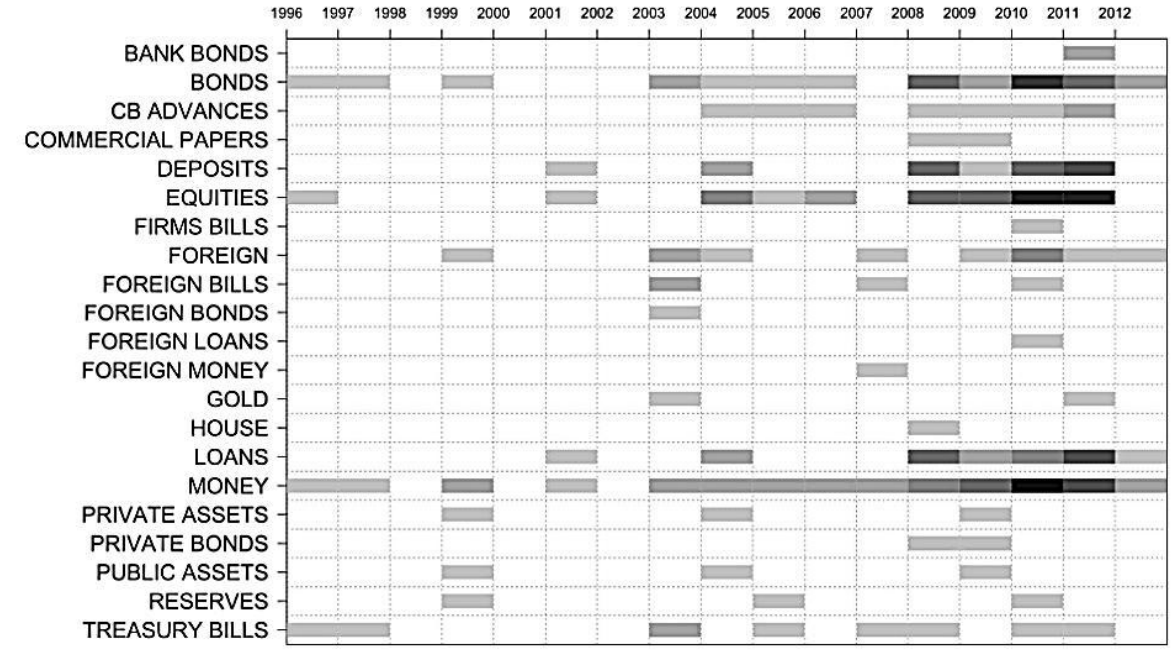
\includegraphics[width = 0.9\textwidth]{Modelo/Caverzassi_Heatmap.png}
    \caption*{\textbf{Fonte:} \textcite[p.~4]{caverzasi_stock-flow_2013}}
\end{figure}


%BREVE REVISÃO MODELOS SHIPMAN + GRÁFICO CAVERZASSI



Feitas essas ressalvas, dada a estrutura contábil e explicitadas as hipóteses (via equações comportamentais), resta seguir para a solução do modelo. Como pontuam \textcite{caverzasi_stock-flow_2013}, existem duas vias: (i) simulação e (ii) discursiva. A primeira delas permite expor de forma mais clara as relações entre as variáveis de modelos mais complexos em que a solução analítica não é facilmente encontrada. No entanto, tal caminho fez com que o grau de complexidade dos modelos simulados fosse exponencializada de modo que a intuição econômica torna-se facilmente turva. Diante destas complicações, o presente capítulo prioriza a parcimônia de modo que serão incluídos apenas os elementos necessários para a narrativa. A justificativa deste procedimento decorre da maior clareza que tal modelagem frente a um menor ``realismo''. Além disso, tal postura permite encontrar soluções analíticas com maior facilidade de modo que são explicitados os parâmetros mais relevantes para as trajetórias de longo prazo. 
Apesar de parcimoniosidade do modelo, a simulação tem a vantagem de fornecer informações que não se restringem às soluções de equilíbrio e que vão além de um sistema de equações em que é possível visualizar as relações entre algumas variáveis de interesse. 
Dito isso, a seção seguinte expõe o modelo que será simulado adiante.
\section{Modelos de crescimento e os gastos autônomos: uma revisão empírica}
\label{RevF}

O objetivo desta seção é analisar os trabalhos empíricos que analisam a relação entre os gastos autônomos não criadores de capacidade produtiva ao setor privado e crescimento econômico e, assim, complementar a discussão teórica realizada na seção \ref{SecAutonomos}. Mais uma vez, seguindo a categorização de \textcite{cesaratto_technical_2003}, os referidos gastos são:
(i) consumo financiado por crédito ou riqueza acumulada;
(ii) gastos do governo;
(iii) investimento residencial;
(iv) exportações e;
(v) gastos com P\&D\footnote{
	%TODO Nota de rodapé sobre gastos com P\&D
	Nota de rodapé sobre gastos com P\&D?
}. 
Da revisão da literatura empírica, verificou-se três principais preocupações: 
\begin{description}
	\item[(a)] testar a importância dos gastos autônomos sobre a taxa de crescimento de longo prazo; 
	\item[(b)] avaliar a relação entre taxa de investimento e produto;
	\item[(c)] investigar a dinâmica de cada um dos gastos autônomos referidos anteriormente.
\end{description}
Cada um desses pontos será analisado adiante. Por fim, vale pontuar que, dados os objetivos desta investigação, serão privilegiados os trabalhos que tenham o supermultiplicador sraffiano desenvolvido por \textcite{serrano_long_1995} e \textcite{bortis_institutions_1996} como forma de análise.

No que diz respeito ao tema (a), o trabalho de \textcite{girardi_long-run_2016} se destaca por analisar os efeitos de longo prazo dos gastos autônomos sobre o produto bem como por apresentar uma forma de se calcular o supermultiplicador para a economia norte-americana. Para tanto, estimam um VECM e obtém os resultados esperados de acordo com a teoria\footnote{Mais precisamente, tais resultados se sustentam uma vez desconsiderado o consumo financiado por crédito. Como justificativa para tal medida, \textcite[p.~13]{girardi_long-run_2016} argumentam que tal gasto está associado a algumas fases do ciclo econômico e, portanto, apresenta uma parcela consideravelmente induzida.}: (i) gastos autônomos e o produto apresentam uma tendência de longo prazo (são cointegradas); (ii) relação de causalidade parte dos gastos autônomos para o produto e (iii) relação positiva entre taxa de crescimento dos gastos autônomos e taxa de investimento. Já no artigo de \textcite{girardi_autonomous_2018}, o mesmo é feito para alguns países da zona do euro com a diferença que foram utilizadas variáveis instrumentais como \textit{proxy} de alguns gastos autônomos e foram obtidos resultados semelhantes ao do estudo anterior. Por fim, o trabalho de \textcite{goes_supermultiplier_2018} possui semelhanças com o de \textcite{girardi_long-run_2016}, mas se distingue por extendê-lo para mais países e por adotar critérios para agrupá-los bem como por reportar a convergência do grau de utilização ao nível normal.

Os trabalhos empíricos envolvendo o supermultiplicador, no entanto, não estão restringidos aos EUA ou países da OCDE. \textcite{freitas_pattern_2013}, por exemplo, analisam o caso brasileiro para os anos de 1970 a 2005 e concluem que diferentes gastos autônomos (em ordem, gastos do governo e consumo financiado por crédito) lideraram o crescimento em momentos distintos. Paralelamente, \textcite{braga_investment_2018} investiga o efeito acelerador para o caso brasileiro de 1996 a 2017 e conclui que o investimento criador de capacidade produtiva é causado (no sentido de Granger) pelo produto, ou seja, é induzido.  

Enquanto \textcite{freitas_pattern_2013} e \textcite{girardi_autonomous_2015} abordam a importância dos gastos autônomos para o crescimento, \textcite{braga_investment_2018} avalia a relação entre taxa de investimento e crescimento. Assim, estão abarcadas as preocupações (a) e (b) elencadas anteriormente. Resta, portanto, evidenciar os trabalhos que destacam a importância de alguns gastos autônomos em específico. Um deles é o de \textcite{medici_cointegration_2011} em que avalia o caso argentino para os anos de 1980 a 2007 e encontra evidências de cointegração entre renda, consumo do governo e o consumo privado autônomo (\textit{i.e.} não assalariado) em que os últimos granger-causam o primeiro. O modelo apresentado por \textcite{deleidi_mission-oriented_2019}, por sua vez, também analisa a importância dos gastos do governo investigando se o tipo de política fiscal adotada tem impactos sobre o crescimento. Em linhas gerais, os autores concluem que gastos orientados em setores mais intensivos em P\&D e em mudanças estrutuais (correspondente ao gasto v) possuem efeitos maiores do que uma política centrada apenas em incentivos fiscais. Já no que diz respeito às exportações (gasto iv), destaca-se a literatura de restrição por balanço de pagamentos seguindo a lei de \textcite{mccombie_balance--payments_1994} 
%TODO Orig year Thirwall
em que as exportações são os determinantes do crescimento de longo prazo \cites{atesoglu_balance--payments-constrained_1993}{mccombie_empirics_1997}{moreno-brid_mexicos_1999}{bertola_balance--payments-constrained_2002}\footnote{Por mais que tal abordagem não lance mão explicitamente do modelo do supermultiplicador sraffiano, as conclusões são compatíveis uma vez que estão presentes gastos autônomos não criadores de capacidade e a especificação da função investimento pode seguir o princípio do ajuste do estoque de capital.}.

%======================== Investimento residencial: Arestis e gasto induzido

Por fim, no que tange o investimento residencial, verifica-se uma lacuna na literatura empírica heterodoxa de crescimento liderado pela demanda. Vale retomar a compatibilidade deste componente da demanda com o modelo do supermultiplicador uma vez que (i) não cria   capacidade produtiva ao setor privado e (ii) pelas hipotecas serem a principal forma de financiamento (e não salários) de acordo com o \textit{Survey of Construction} \cite{us_census_bureau_characteristics_2017}. Dito isso, caberá a seção seguinte examinar as formas que a literatura econométrica encontrou para incorporar o investimento residencial para então eleger uma alternativa compatível com o supermultiplicador sraffiano.
\section{Investimento residencial e dinâmica macroeconômica}
\label{Secao_Residencial}

Esta seção busca ilustrar a importância do investimento residencial para o crescimento e ciclo econômico norte-americano. 
Uma vez pontuada a relevância deste gasto para a dinâmica macroeconômica norte-americana, cabe discutir quais são seus determinantes de acordo com a literatura para então selecionar a especificação a ser testada adiante.
Dito isso, a subseção seguinte pontua alguns fatos estilizados enquanto a revisão econométrica fica a cargo da seção \ref{RevEmpirica}.

\subsection{Fatos estilizados da economia norte-americana}\label{FatosEUA}

Por uma série de razões\footnote{Dentre as razões pelas quais tal gasto é tão estudado, destacam-se tanto sua elevada volatilidade e considerável participação no PIB quanto a influência de Keynes a respeito do investimento ser a \textit{causa causans}.}, o investimento produtivo é um dos componentes da demanda agregada que mais tem recebido atenção (ao menos) entre macroeconomistas heterodoxos de modo que a importância outros gastos têm sido subestimada \cite{brochier_macroeconomics_2017}.
O investimento residencial é um desses casos que não é tão investigado pela literatura e nem possui uma participação elevada na renda (gráfico \ref{FigAutonomos}), mas é mais volátil que o PIB e que o investimento das firmas (gráfico \ref{FigVolatilidade}). 
O principal objetivo desta seção é destacar que a pouca atenção dada ao investimento residencial não é compatível com seu grau de importância para a economia norte-americana e que esta relevância não se restringe à crise imobiliária recente.
%Adicionalmente, procura-se mostrar que, ao contrário de \textcite{grebler_capital_1956}, tal relevância não só não se apequenou como tem se amplificado  \cites{fiebiger_semi-autonomous_2018}{karwowski_financialisation_2019}{walther_forty_2019}.
Em paralelo, serão apresentados alguns fatos estilizados que irão contextualizar as simulações do capítulo \ref{CapModelo}.



%%%%%%%%%%%%%%%%%%%%%%%%%%%%% PEQUENA PARTICIPAÇÃO NO PIB %%%%%%%%%%%%%%%%%%%%%%%%%%%

\begin{figure}[H]
	\centering
	\caption{Participação dos gastos autônomos no PIB dos EUA (1979-2019)}
	\label{FigAutonomos}
	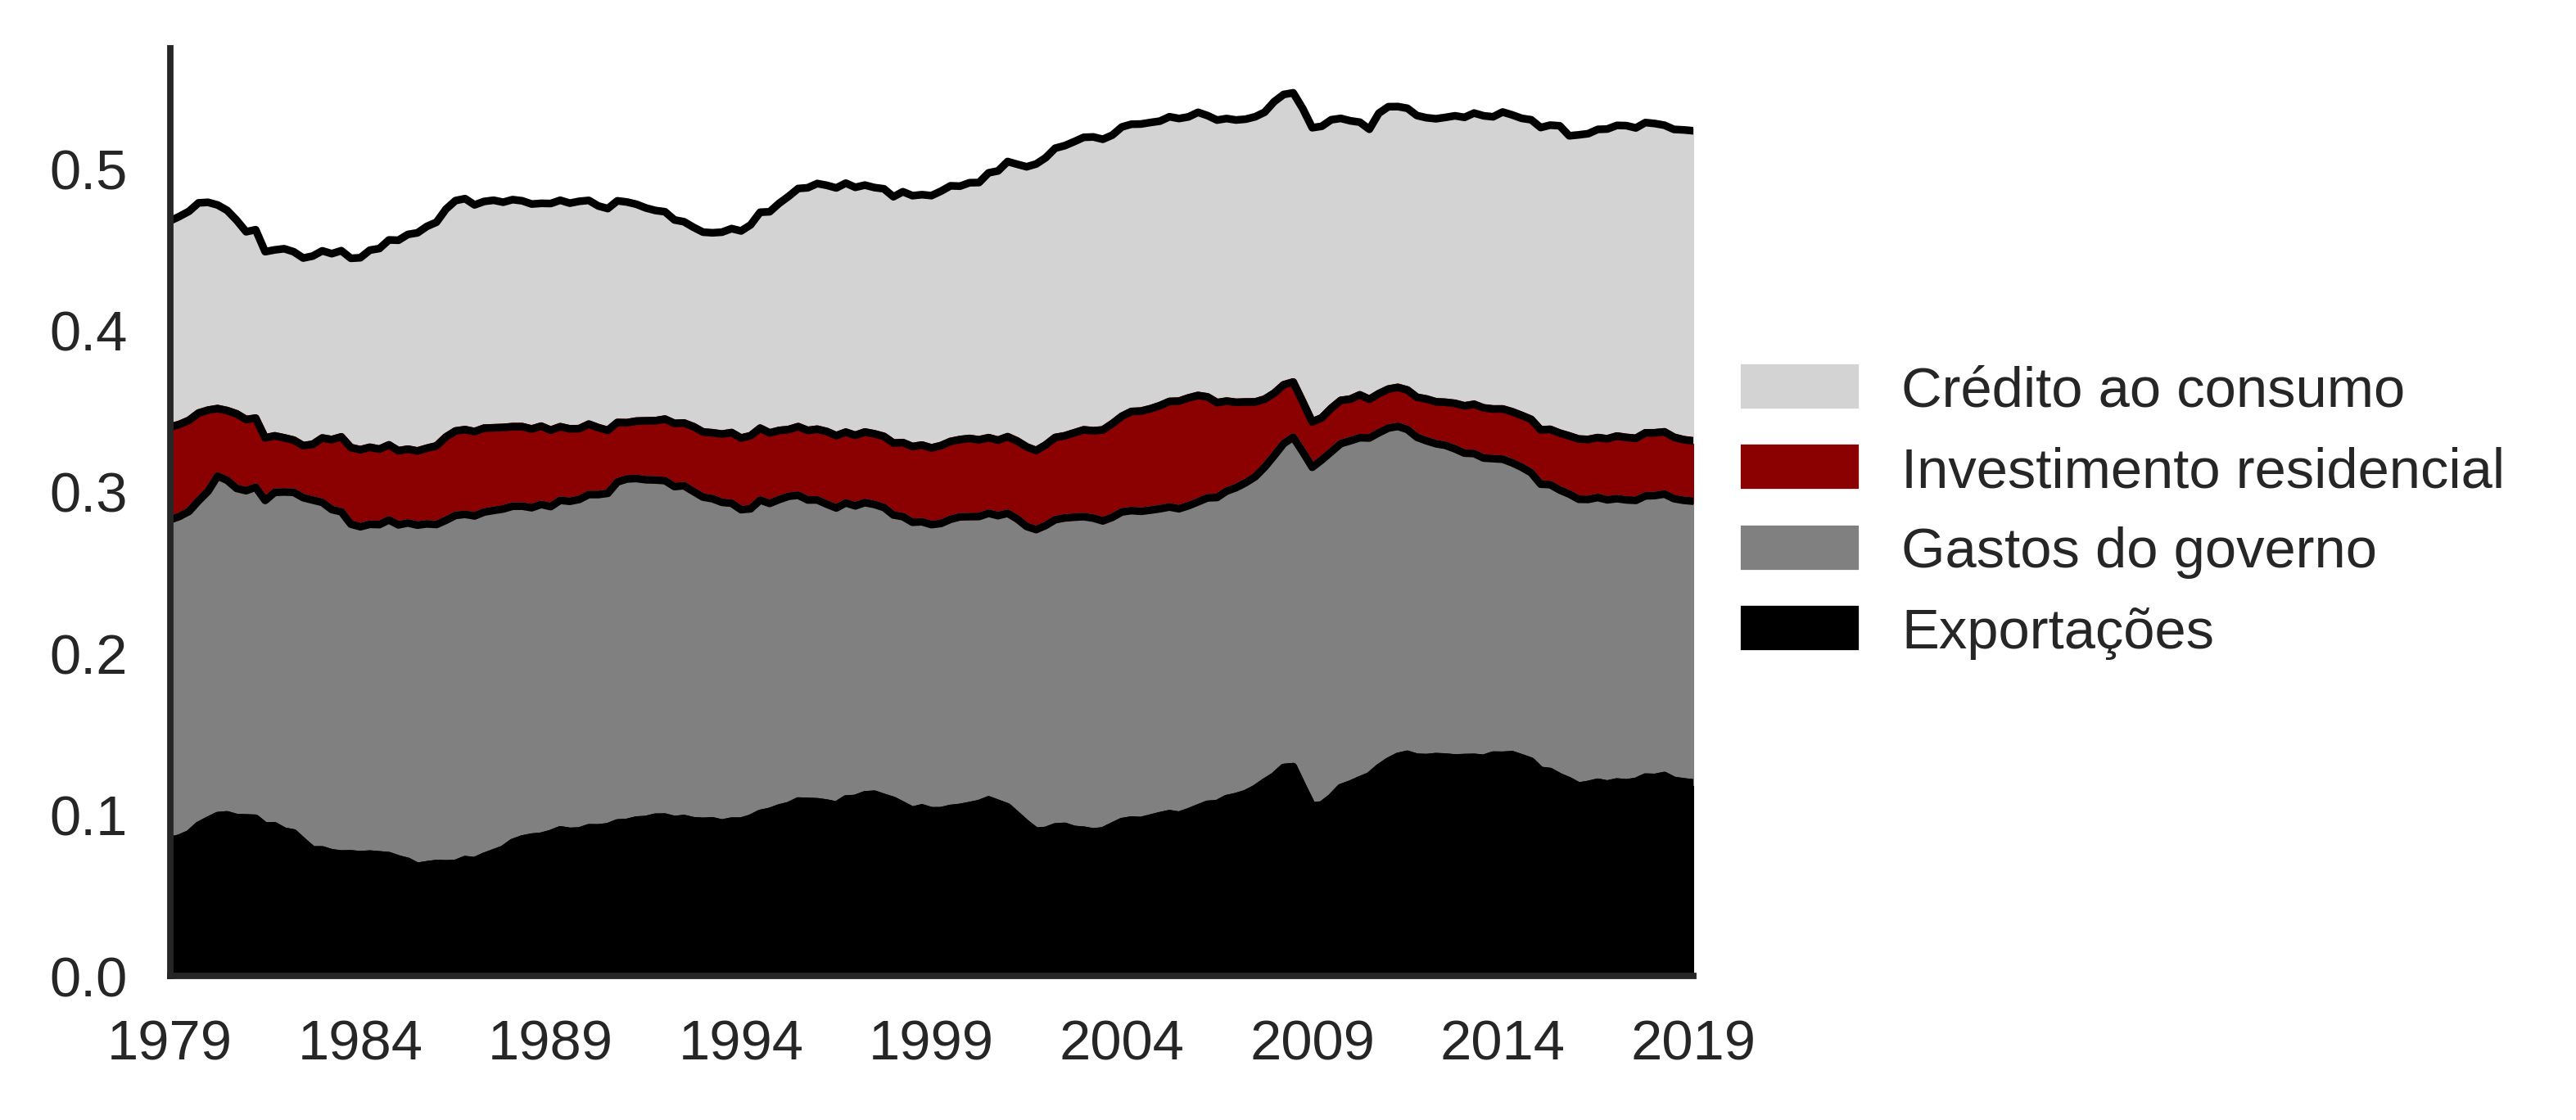
\includegraphics[width=\textwidth]{../../Dados/Fatos_Estilizados/figs/Gastos_autonomos.png}
	\caption*{\textbf{Fonte:} U.S. Bureau of Economic Analisys, elaboração própria}
\end{figure}


\begin{figure}[H]
	\centering
	\caption{Distribuição de taxas de crescimento selecionadas (1947-2019)}
	\label{FigVolatilidade}
	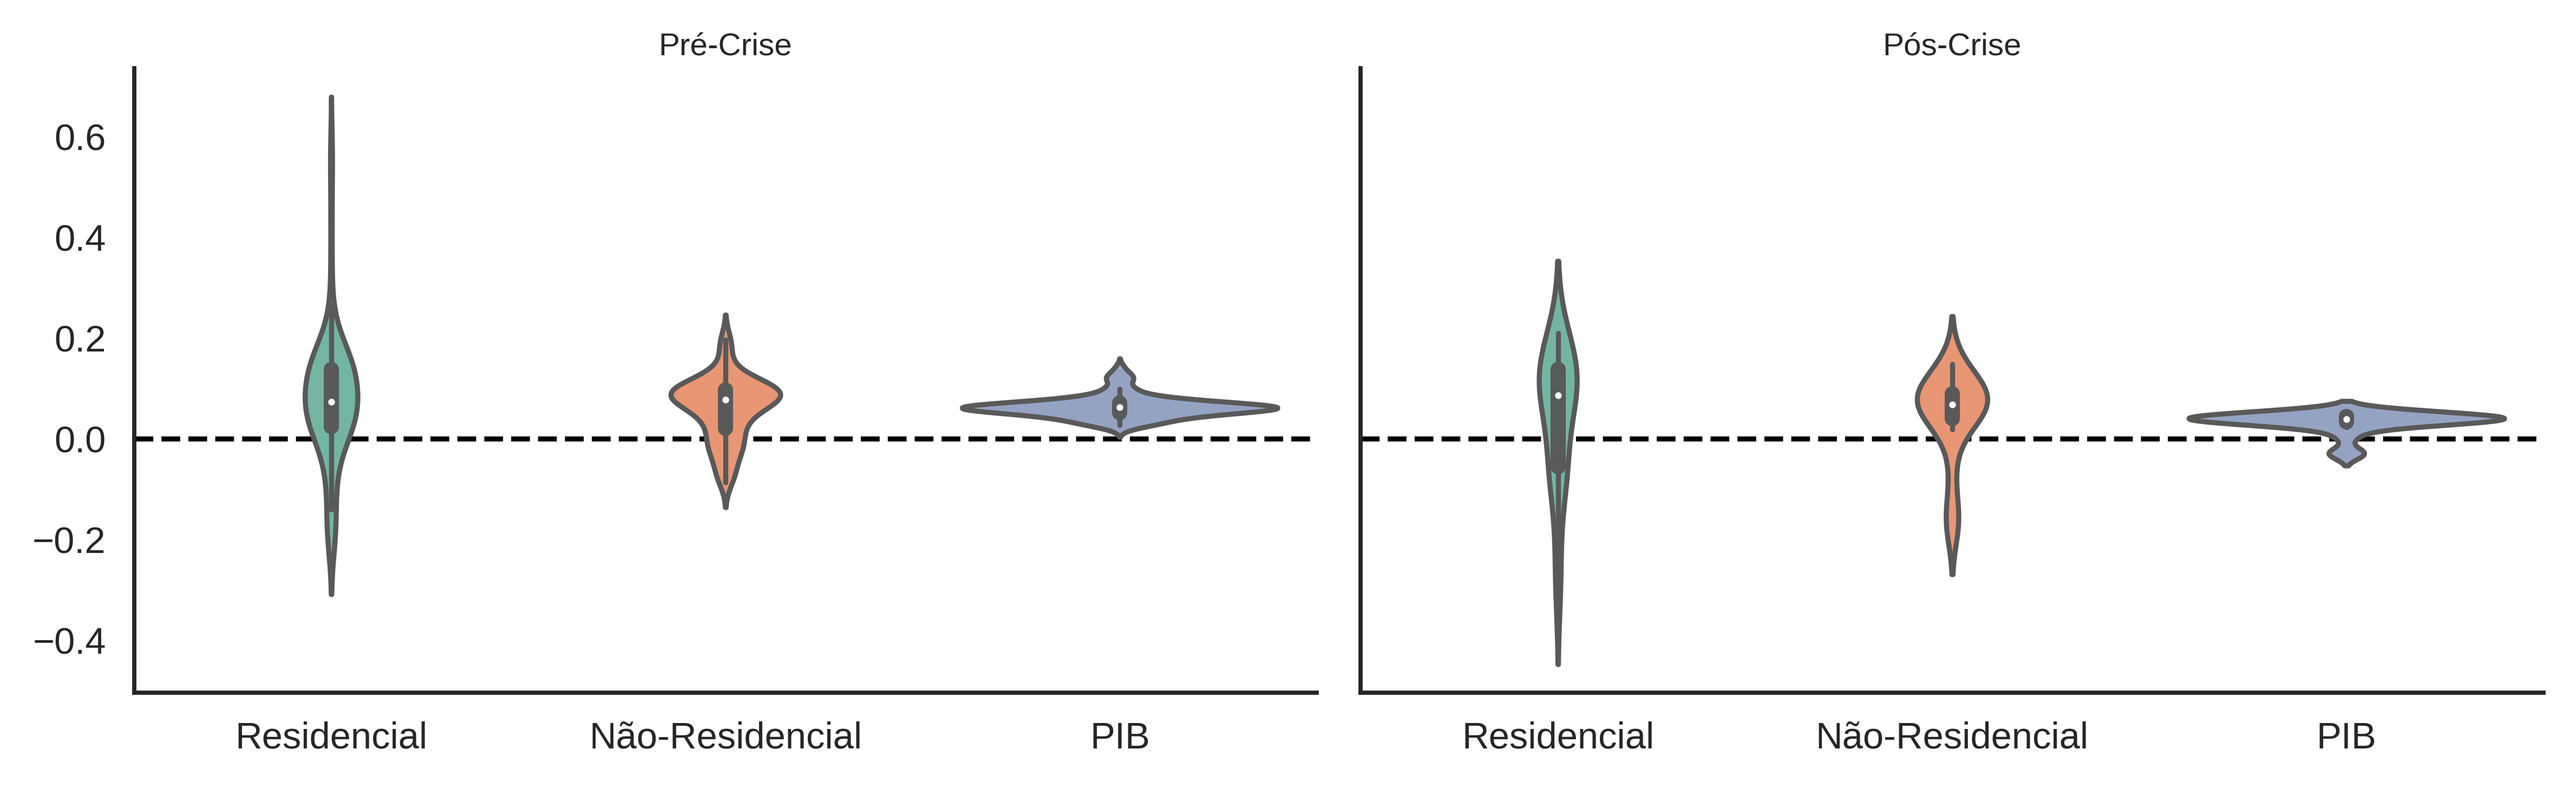
\includegraphics[width=\textwidth]{../../Dados/Fatos_Estilizados/figs/Volatilidade.png}
	\caption*{\textbf{Fonte:} U.S. Bureau of Economic Analisys, elaboração própria}
\end{figure}

Neste ponto, cabe mencionar o ineditismo de \textcite{green_follow_1997} e \textcite{leamer_housing_2007} --- e revisitado em \textcite{leamer_housing_2015} e por \textcite{fiebiger_trend_2017} --- ao lançar luz sobre a importância do investimento residencial na determinação dos ciclos econômicos antes mesmo da Grande Recessão. 
Ao avaliar o caso norte-americano, \textcite{green_follow_1997} conclui que o
investimento residencial antecipa --- mais que o investimento das firmas --- o ciclo econômico, mas, ao mesmo tempo, reconhece que isso não implica o estabelecimento de uma relação causal. Na tentativa de compreender tais resultados, afirma:

\begin{citacao}
	
	[P]erhaps residential investiment, like stock prices and interest rates, is a good predictor of GDP because it is a series that reflects \textbf{foward looking behavior}. Presumably households will not increase their expenditures on housing unless they expect to prosper in the future. Building a house is a natural mechanism for doing this. Thus, the series can do a good job of predicting GDP without necessarily causing GDP.
	\cite[p.~267, grifos adicionados]{green_follow_1997}
\end{citacao}
Apesar de dar atenção para um gasto não criador de capacidade, \textcite{green_follow_1997} argumenta que o investimento residencial não antecipa crescimento econômico e indicaria apenas uma precedência temporal, ou seja, contribui para prever a trajetória da renda sem necessariamente causá-la.
\textcite{leamer_housing_2007}, por sua vez, avança em direção a relação de causalidade entre este gasto e o PIB. Grosso modo, afirma que a construção de novos imóveis implica maior consumo de bens duráveis e, portanto, trata-se de um ciclo decorrente do \textit{volume} e não do preço dos imóveis. 

Uma forma de visualizar a importância do investimento residencial para o ciclo econômico na economia estadunidense é por meio do gráfico \ref{FigIh_u} em que cada um dos painéis apresenta um ciclo iniciado no primeiro trimestre de crescimento positivo após a recessão e se estende até o fim da recessão seguinte\footnote{
	Raciocínio semelhante pode ser encontrado em \textcite{fiebiger_semi-autonomous_2018} em que, diferentemente do presente trabalho, não é incluído consumo financiado por crédito.}. 
No eixo vertical, observa-se a participação desse gasto no PIB, enquanto no eixo horizontal, o grau de utilização da capacidade como uma \textit{proxy} para o ciclo econômico. Exceto para o período 1991-2001, a recuperação (aumento da utilização da capacidade) é caracterizada por uma taxa de crescimento do investimento residencial maior que o crescimento da economia, resultando em maior participação desse gasto no PIB. Considerando que as firmas seguem o princípio do ajuste do estoque de capital, ampliam a taxa de acumulação de modo a ajustar o grau de utilização para o grau normal. O aumento da taxa de crescimento do investimento das firmas e de outros gastos reduz a participação do investimento residencial no PIB. A maturação do investimento das firmas, por sua vez, redunda em menor utilização da capacidade produtiva\footnote{
	Complementarmente, os trabalhos de \textcite{fiebiger_semi-autonomous_2018} e \textcite{fiebiger_trend_2017} também reportam o investimento residencial como determinante do comportamento cíclico e adicionam o consumo financiado por crédito a essa dinâmica. Além disso, apresentam uma similaridade com \textcite{dejuan_hidden_2017} e \textcite{teixeira_crescimento_2015} para os quais a instabilidade econômica está associada à instabilidade (ao menos de alguns) gastos autônomos e não do investimento das firmas, que segue o princípio do ajuste do estoque de capital.}. 
Com o deflagrar da crise, o grau de utilização cai e o ciclo se encerra no fim da recessão e se reinicia --- no painel seguinte --- com a economia sendo puxada pelo investimento residencial.
Em resumo, tais gráficos denotam uma especifidade do ciclo econômico norte-americano que pode ser resumida nos seguintes termos: ``\textit{[f]irst homes, then cars, and last business equipment}'' \cite[p.~8]{leamer_housing_2007}.




\begin{figure}[H]
	\centering
	\caption{Relação entre taxa de investimento residencial e grau de utilização por recessão}
	\label{FigIh_u}
	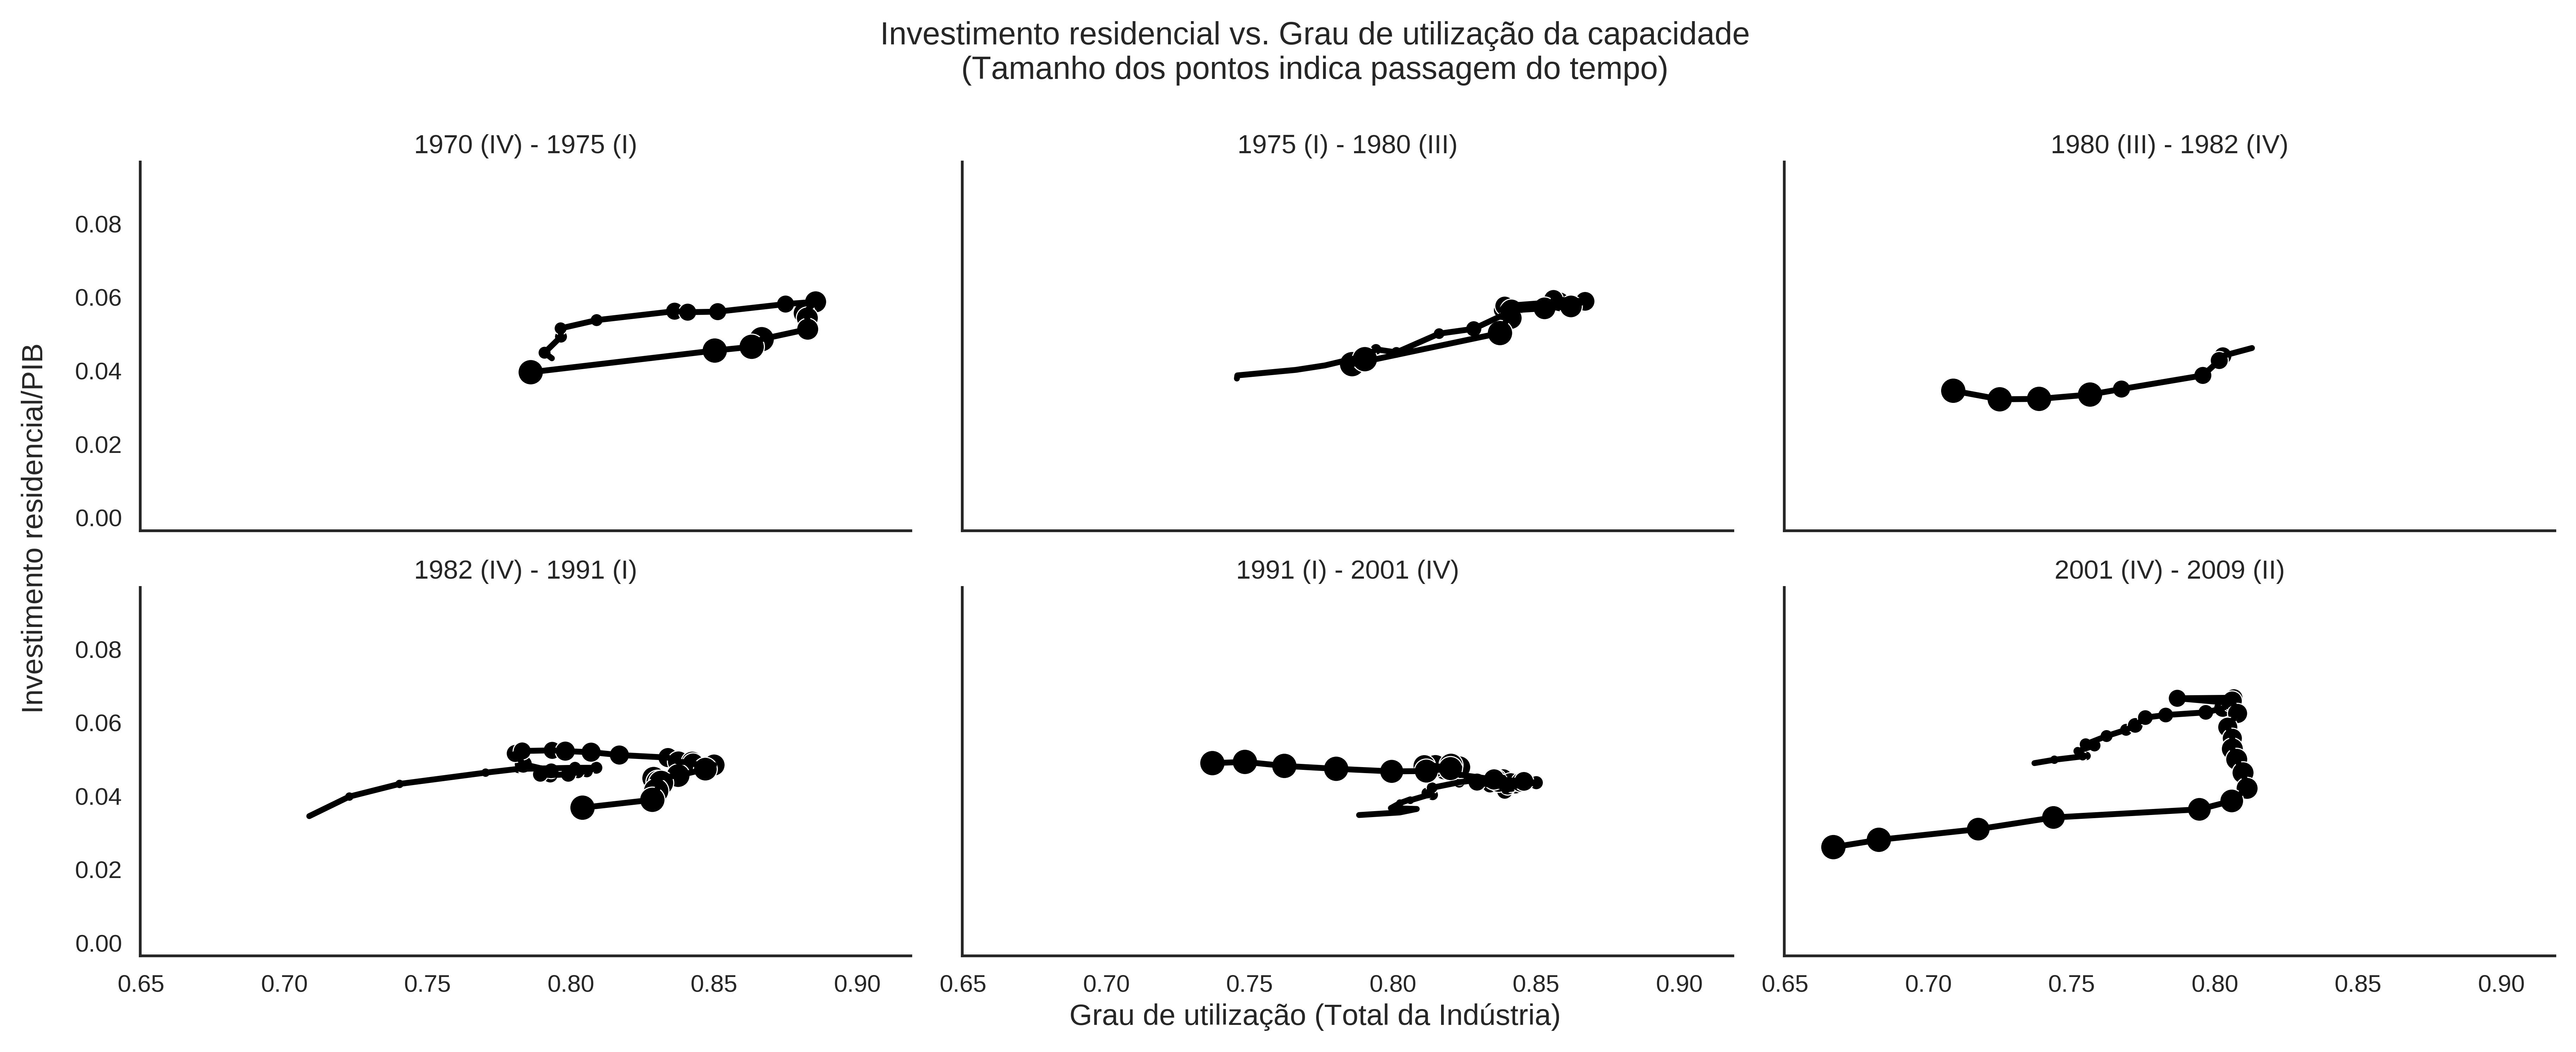
\includegraphics[width=\textwidth]{../../Dados/Fatos_Estilizados/figs/Ciclo_Ih_u.png}
	\caption*{\textbf{Fonte:} Elaboração própria}
\end{figure}

%%%%%%%%%%%%%%%%%%%%%%% GRÁFICO RELÓGIO DURÁVEIS %%%%%%%%%%%%%%%%%%

%Como mencionado anteriormente, além de liderar o ciclo econômico, o investimento residencial também está relacionado com o consumo de bens duráveis.
%O gráfico \ref{FigInvesto_Duraveis} ilustra tal associação em que é feita a mesma periodização das crises dos painéis anteriores com a diferença de que o eixo horizontal apresenta a participação do consumo de bens duráveis na renda. 
%Diferentemente do gráfico anterior, este não apresenta um comportamento cíclico tão demarcado ao longo do período que antecedeu a Grande Recessão. Apesar disso, é possível visualizar que a economia desacelera na medida que estes gastos decrescem (conjuntamente) enquanto o crescimento conjunto destes gastos na recuperação não é tão evidente em todos os ciclos (destaque para o ciclo de 1975 a 1980).

%\begin{figure}[H]
%	\centering
%	\caption{Relação entre taxa de investimento residencial e grau de utilização por recessão}
%	\label{FigInvesto_Duraveis}
%	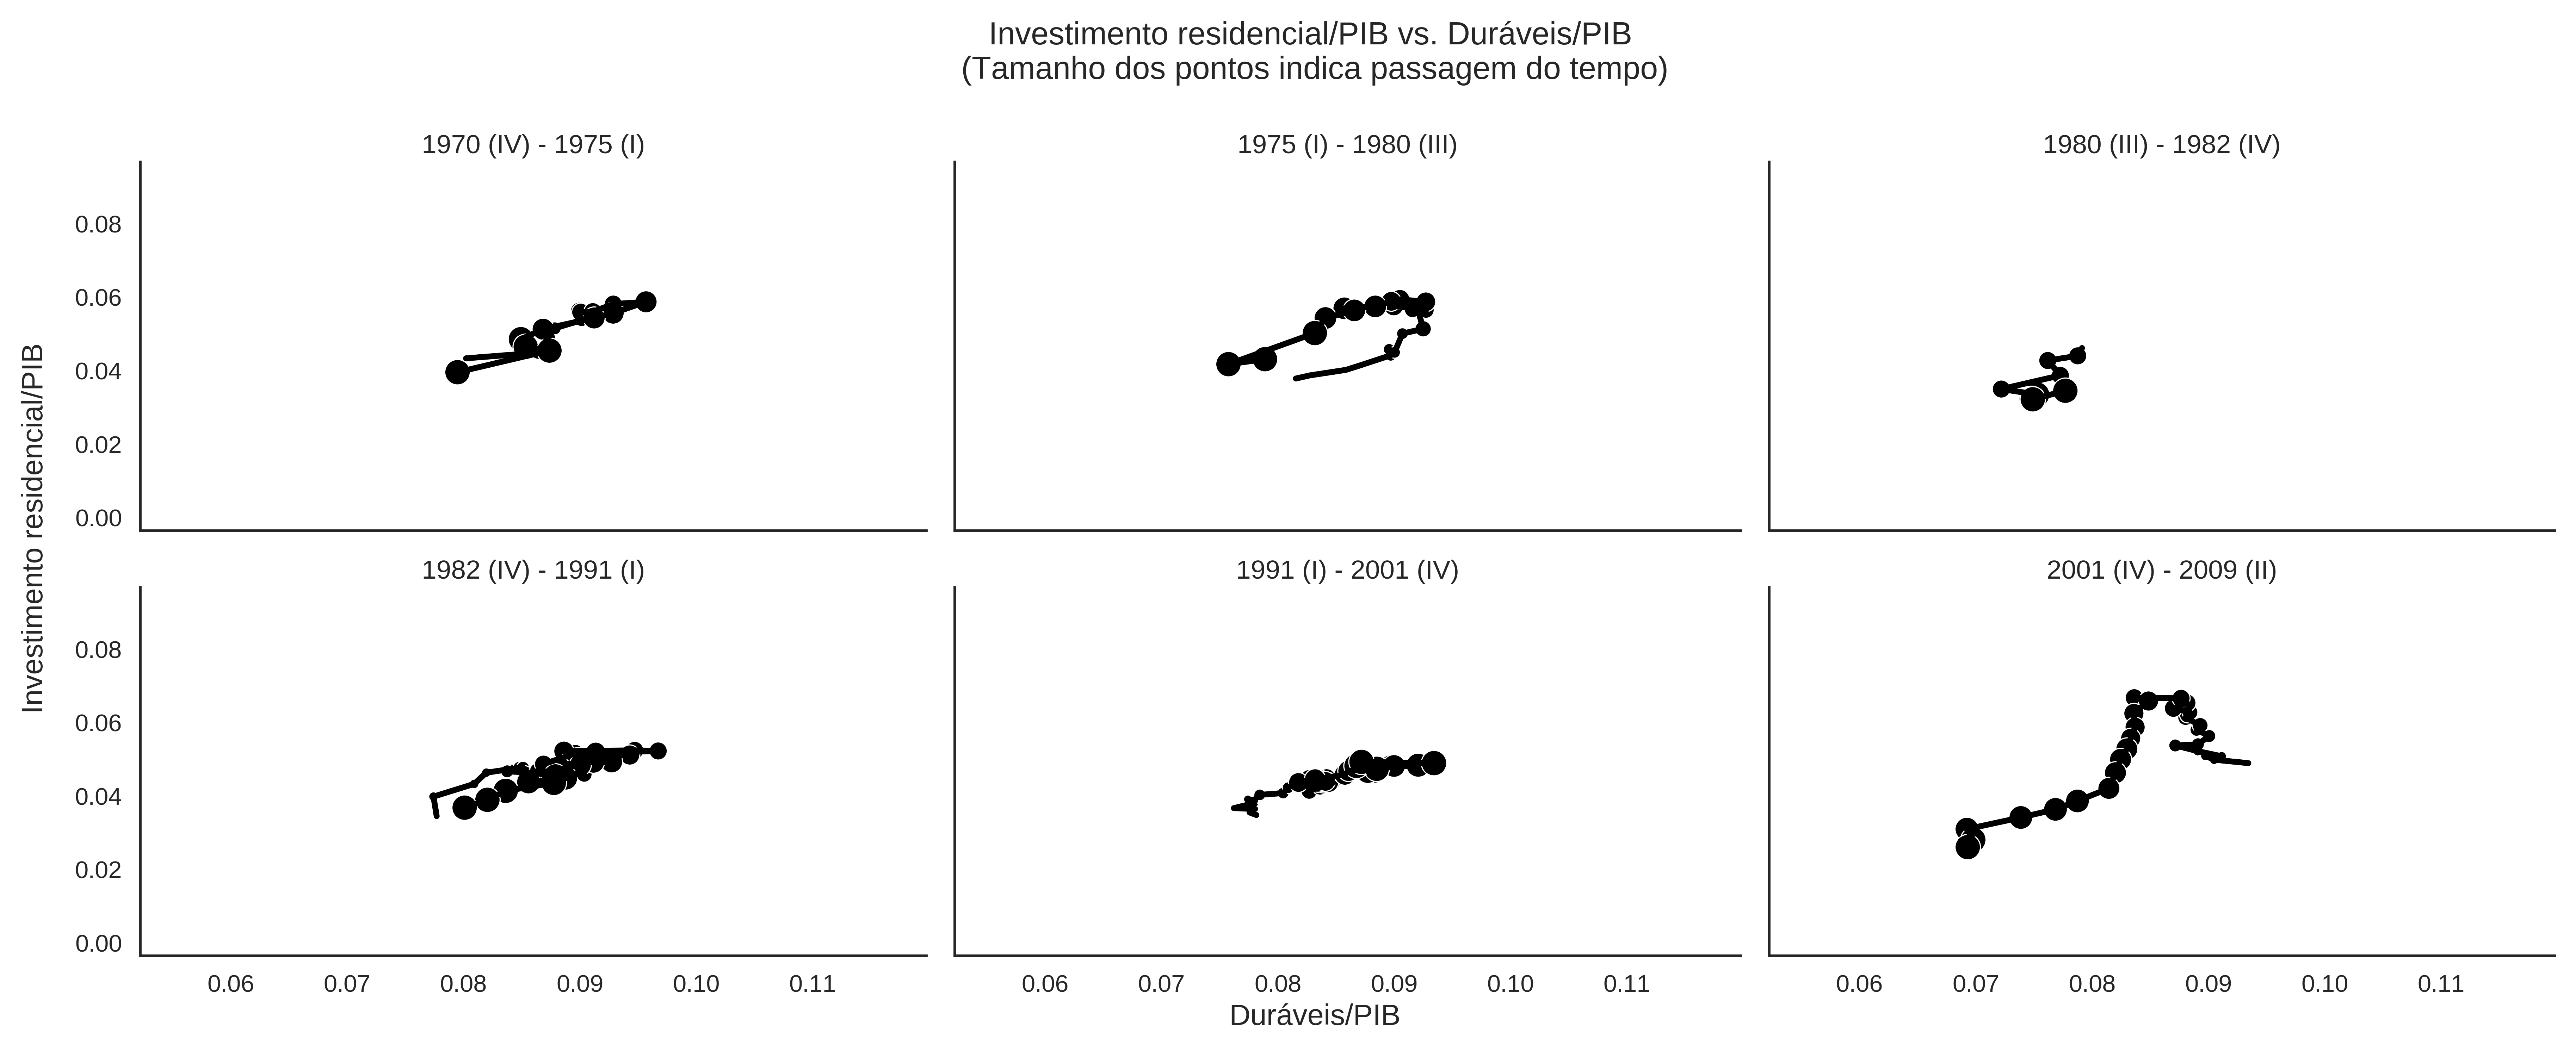
\includegraphics[width=\textwidth]{../../Dados/Fatos_Estilizados/figs/Ciclo_Ih_Duraveis.png}
%	\caption*{\textbf{Fonte:} Elaboração própria}
%\end{figure}

Desse modo, conclui-se que o investimento residencial ajuda a compreender os ciclos econômicos americanos.
Esta dinâmica pode ser visualizada também nos gráficos \ref{FigCriseNorm} e \ref{FigRecuperacaoNorm} em que são apresentadas as taxas de crescimento do produto, consumo financiado por crédito, investimento residencial e não-residencial (normalizadas para manter a comparabilidade)\footnote{
	Nestes gráficos, as taxas de crescimento são normalizadas para facilitar a comparabilidade uma vez que é mantida uma mesma escala uma vez que o investimento residencial apresenta uma taxa de crescimento mais ampla em relação às demais. 
	Dito isso, normalizou-se a taxa de crescimento por seu respectivo desvio-padrão.
} nos trimestres que antecedem e sucedem as recessões/recuperações. 
Destaca-se a redução da taxa de crescimento do investimento residencial nos trimestres que antecedem as recessões enquanto passa a ter taxas positivas antes das recuperações, liderando-as.
Em outras palavras, observa-se que o investimento residencial possui uma taxa de crescimento (a taxas crescentes) positiva nos trimestres que antecedem a recuperação enquanto o investimento das firmas só apresenta tal comportamento adiante. Portanto, esse gráfico ilustra tanto a capacidade do investimento residencial liderar o ciclo quanto a indução do investimento criador de capacidade produtiva.


\begin{figure}[H]
	\centering
	\caption{Taxas de crescimento 4 trimestres antes e depois do início da  \textbf{recessão} (normalizadas para manter a comparabilidade)}
	\label{FigCriseNorm}
	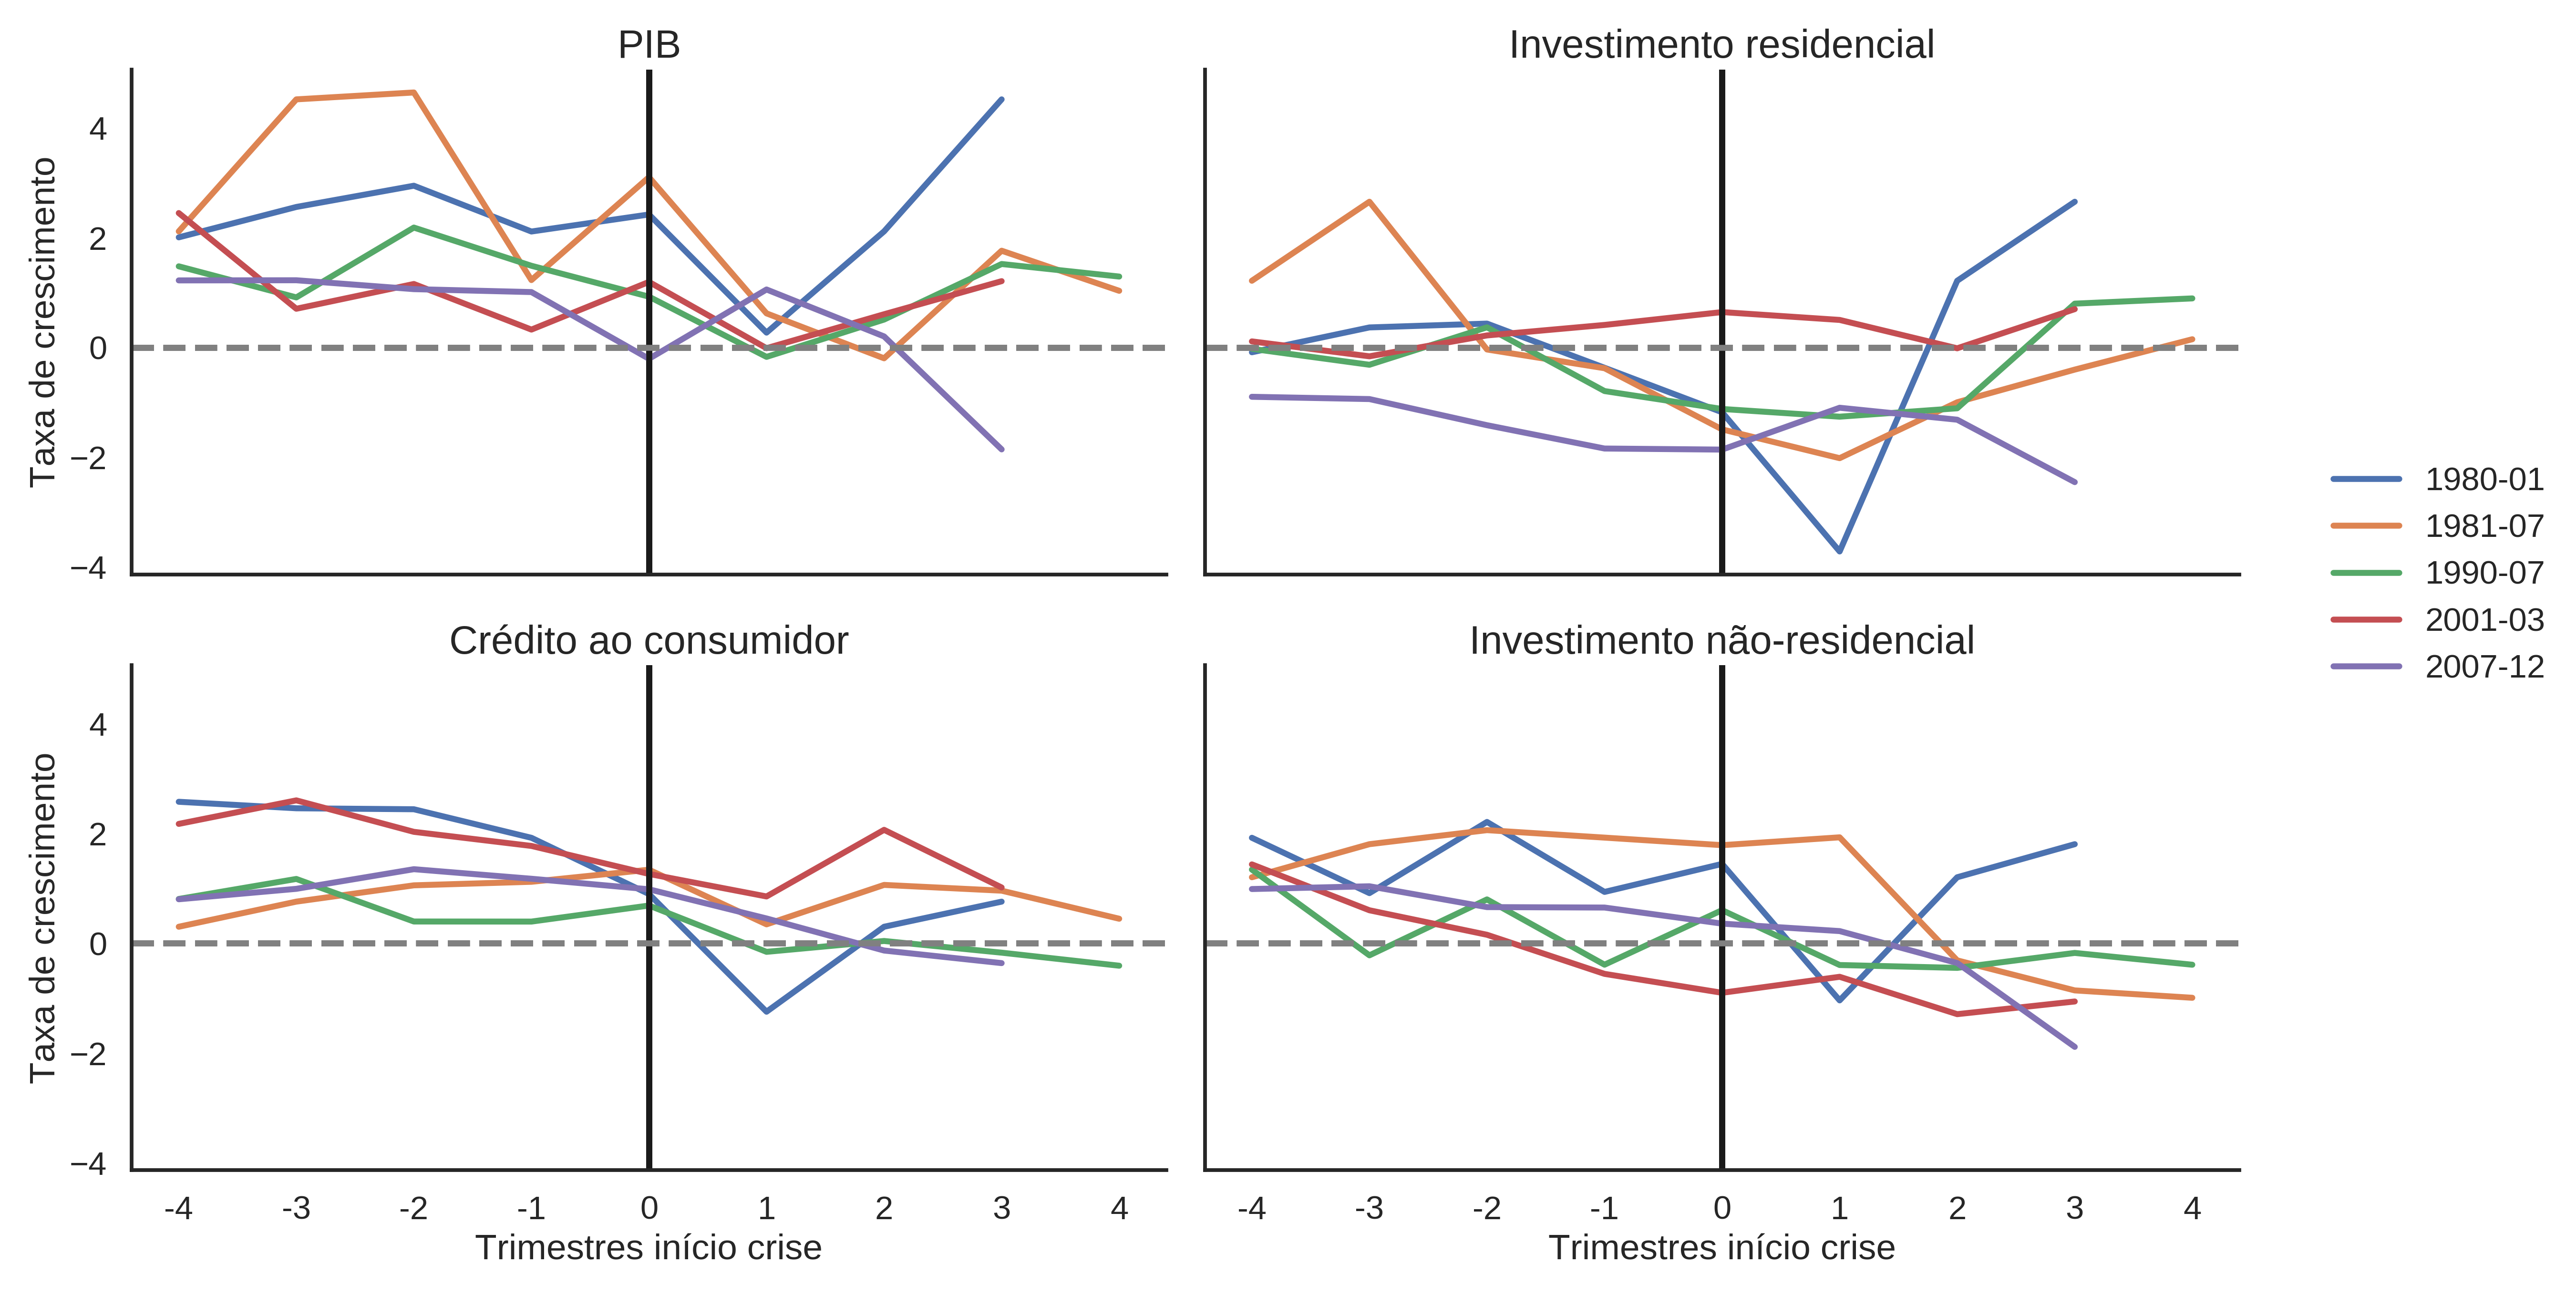
\includegraphics[width=\textwidth]{../../Dados/Fatos_Estilizados/figs/Centrado_Inicio_Norm.png}
	\caption*{\textbf{Fonte:} Elaboração própria}
\end{figure}

\begin{figure}[H]
	\centering
	\caption{Taxas de crescimento 4 trimestres antes e depois do início da  \textbf{recuperação} (normalizadas para manter a comparabilidade)}
	\label{FigRecuperacaoNorm}
	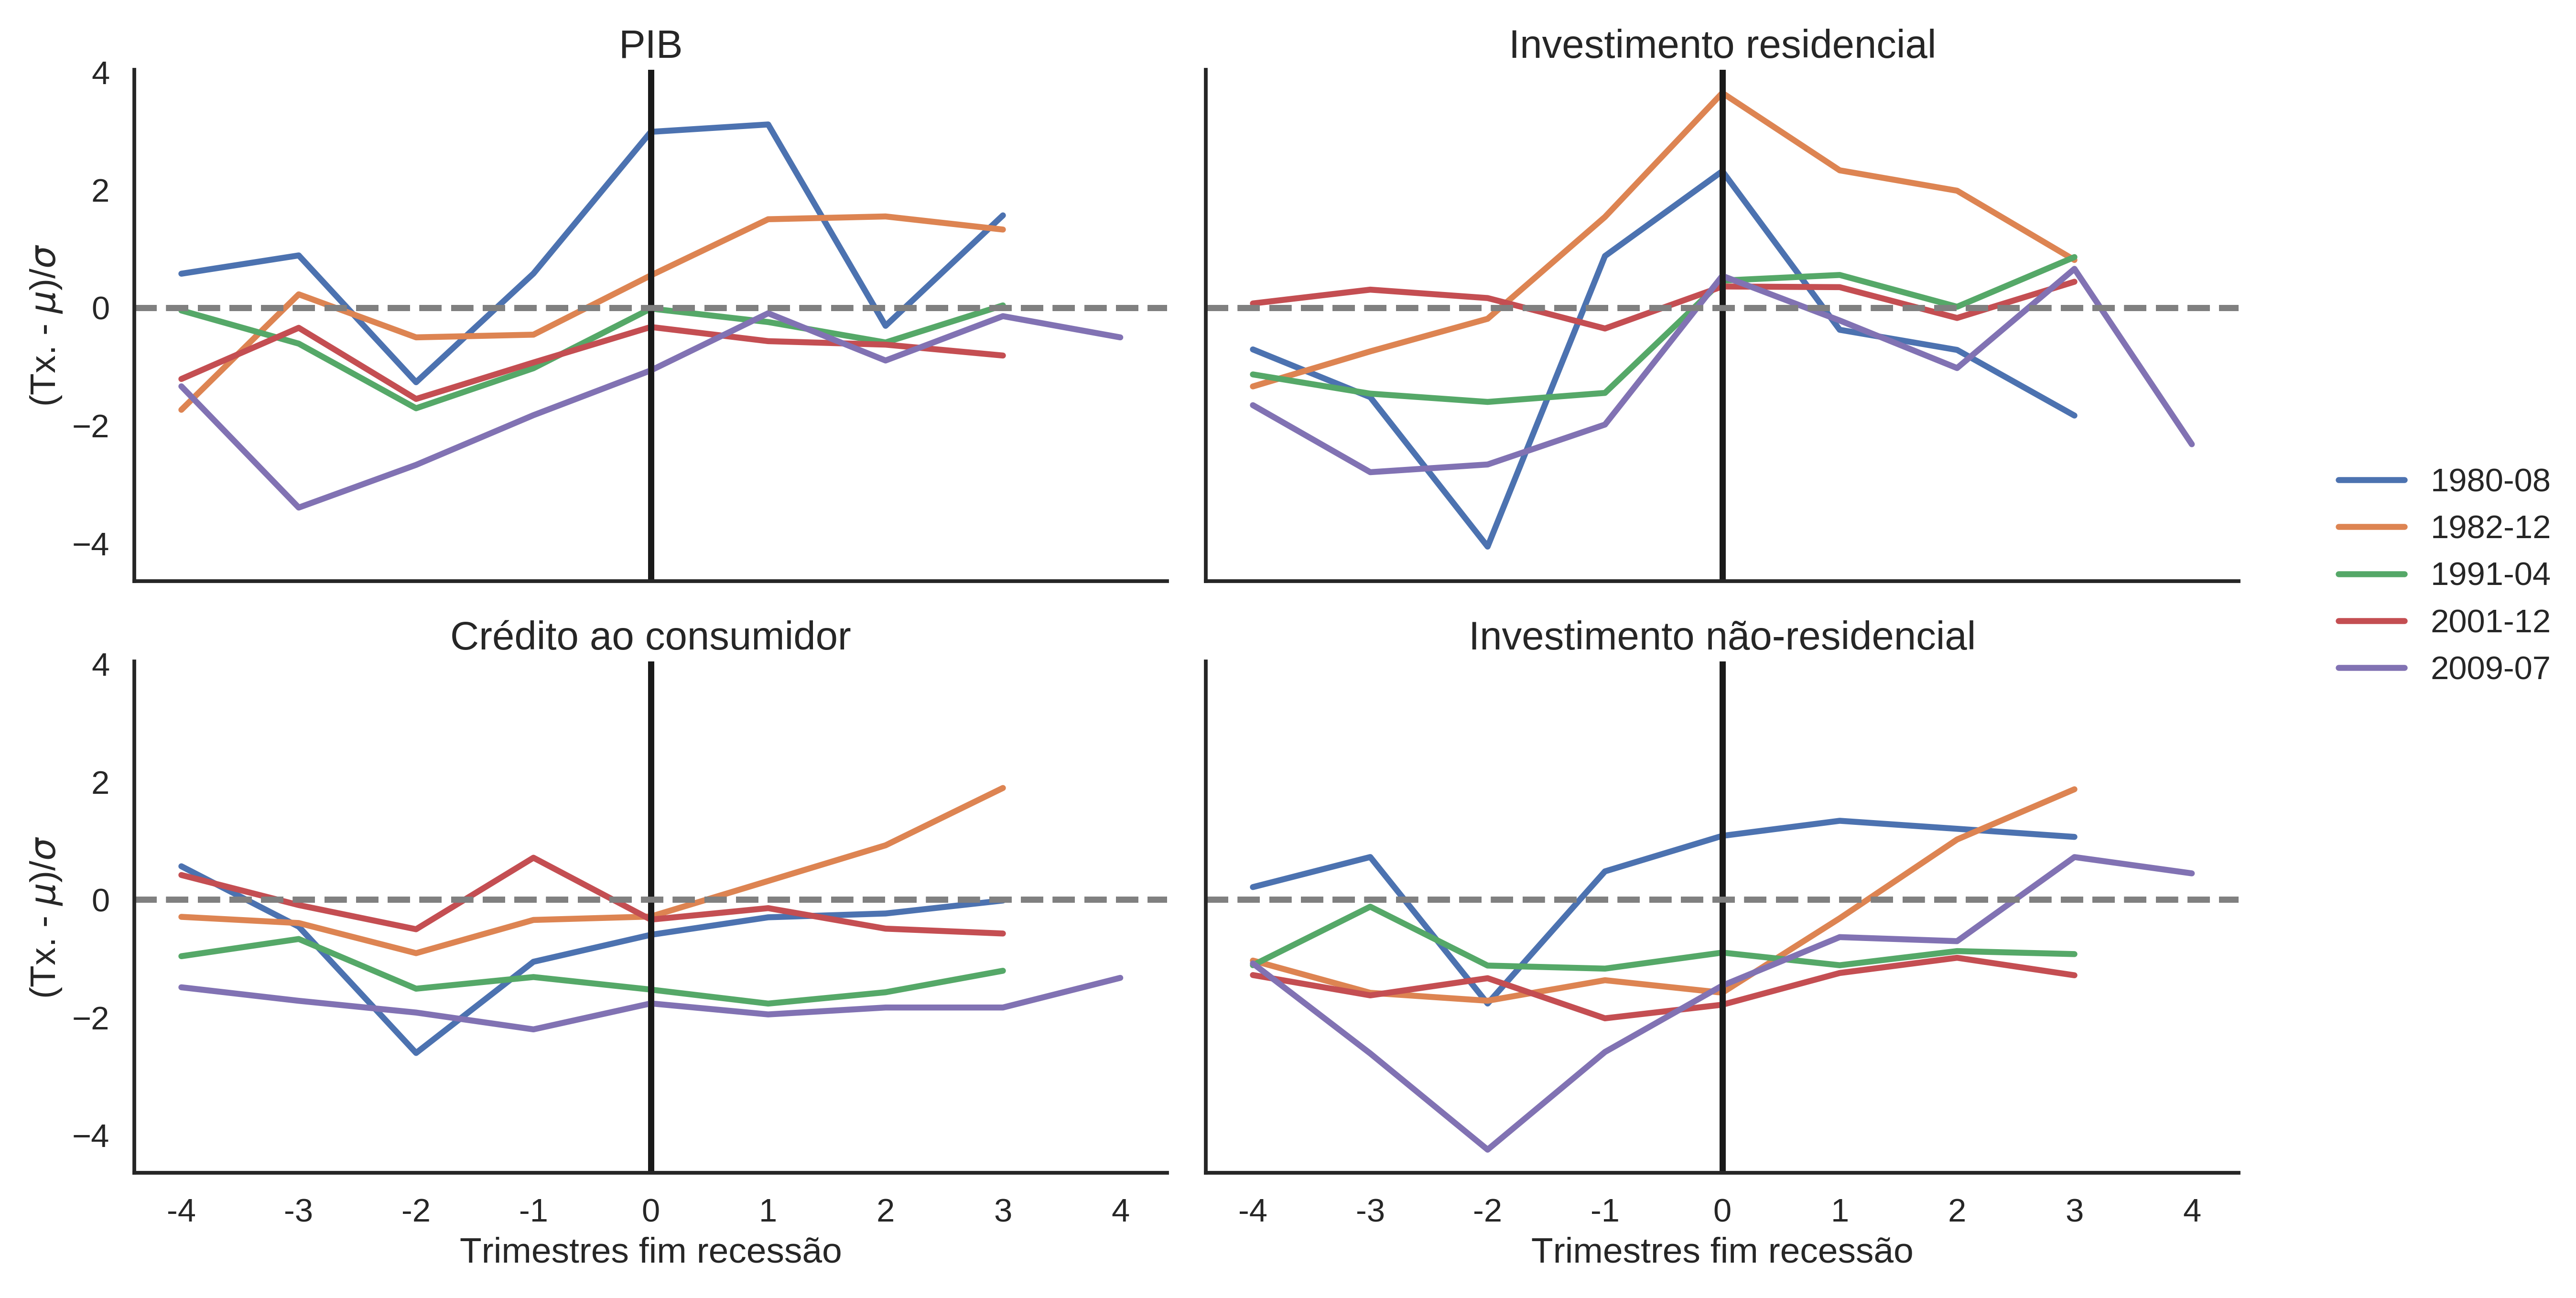
\includegraphics[width=\textwidth]{../../Dados/Fatos_Estilizados/figs/Centrado_Fim_Norm.png}
	\caption*{\textbf{Fonte:} Elaboração própria}
\end{figure}

%TODO Melhorar resolução do gráfico e linhas


Da discussão anterior, conclui-se que a caracterização do ciclo econômico como liderado pelo investimento residencial é bastante extensa uma vez que apresenta esta configuração ao menos desde o pós-guerra.
Apresentada a importância do investimento residencial, resta pontuar alguns fatos estilizados da economia norte-americana que servirão de inspiração para a simulação no capítulo \ref{CapModelo}. 
%No entanto, ocorreram mudanças significantes --- que não anulam a relevância do investimento residencial --- na economia norte-americana no pós-década de 80 que precisam ser analisadas em maior detalhe.
%Um primeiro elemento é a estagnação salarial e os respectivos efeitos sobre o endividamento das famílias na calda inferior da distribuição \cites{barba_rising_2009}{teixeira_uma_2011}. 
%Este endividamento, no entanto, não foi destinado a uma ampliação desproporcional do consumo, mas sim para a preservação do consumo habitual das famílias
%\cites{wolf_rising_2010}{cynamon_inequality_2013}.
Um deles é a evolução dos ativos por percentis da riqueza (gráfico \ref{FigDistAtivos}) em que se destaca o aumento da participação relativa dos imóveis
nos 50\% mais pobres se comparado com 1979 até meados dos anos 90 ---  comportamento este espelhado pelos 1\% mais ricos. 
%Em outras palavras, os imóveis passaram a compor uma parcela cada vez maior do portfólio de ativos deste estrato enquanto os ativos financeiros apresentaram uma tendência de queda persistente.
Enquanto a participação dos imóveis dentre os mais pobres foi crescente e oscilante ao longo do período, o mesmo não pode ser dito sobre os bens duráveis.
Além disso, este gráfico também sugere que a demanda por imóveis por motivos especulativos foi iniciada pelo estrato dos 1\% mais ricos e acompanhada pelo subsequente aumento na demanda por imóveis --- não necessariamente especulativa --- dos 50\% mais pobres associada à expansão do crédito e à desregulamentação financeira.


%\begin{figure}[H]
%	\centering
%	\caption{Distribuição pessoal da renda (percentis selecionados, jan/1980 = 100)}
%	\label{FigDistPessoal}
%	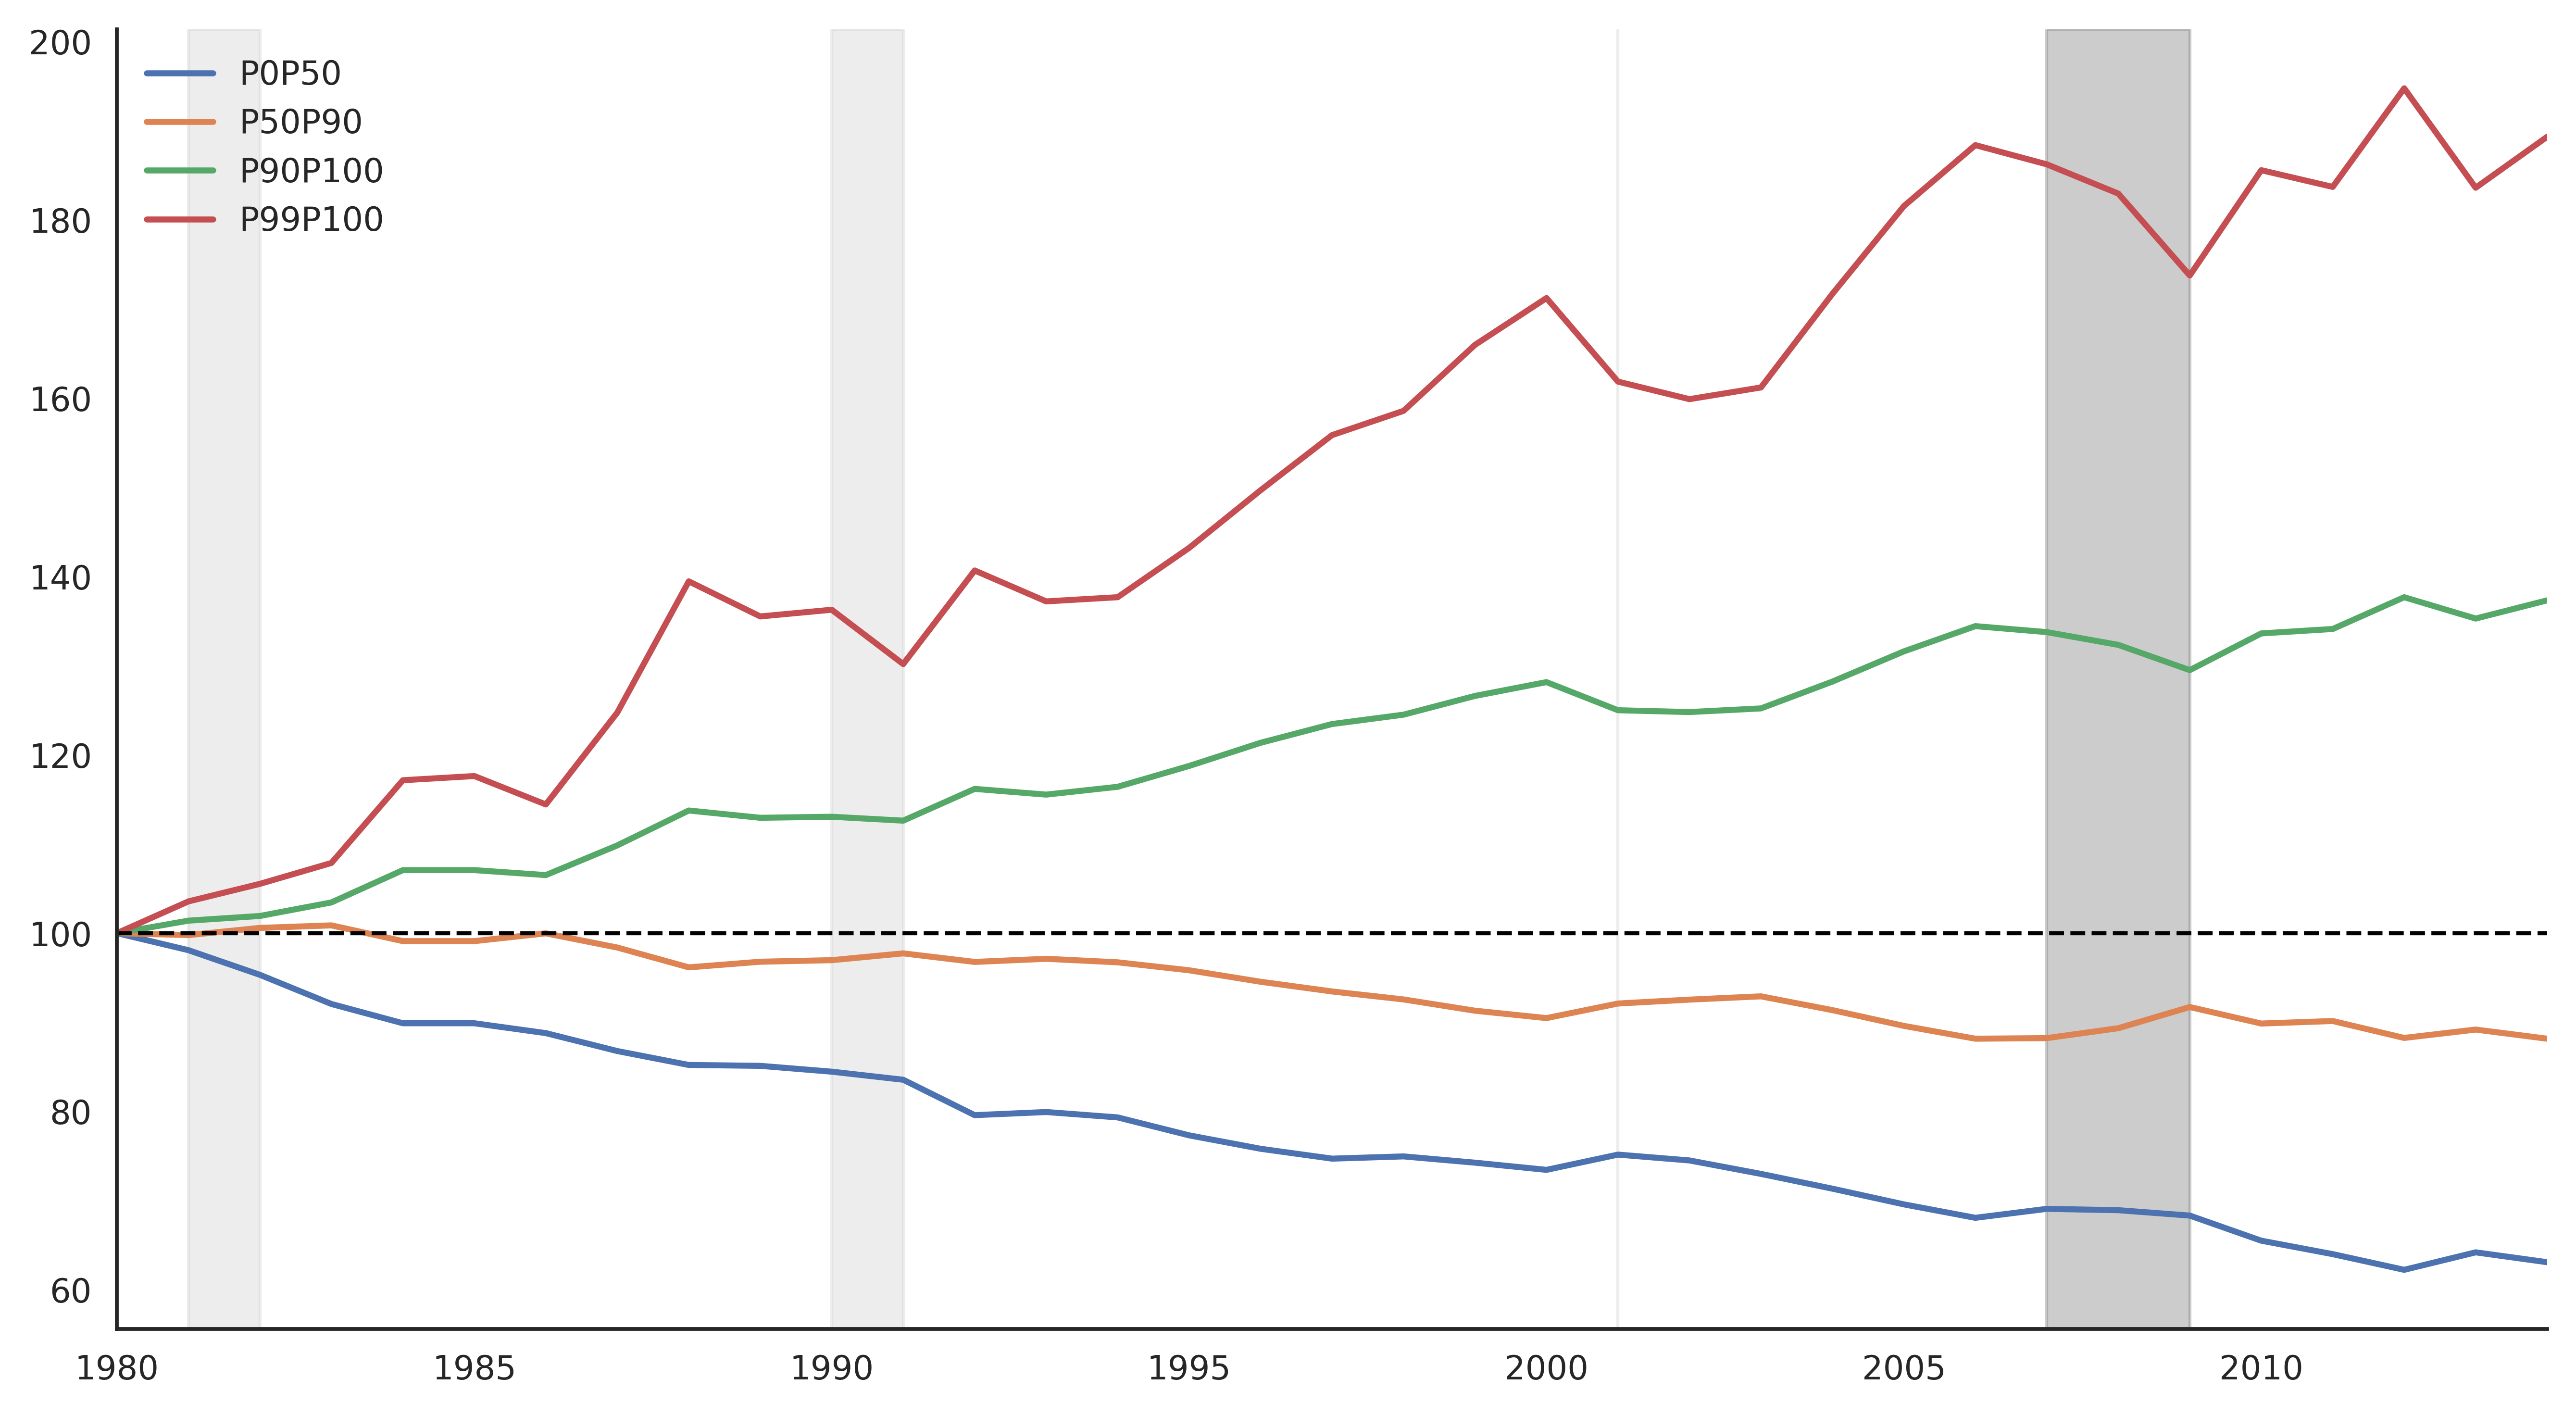
\includegraphics[width=\textwidth]{../../Dados/Fatos_Estilizados/figs/Dist_Pessoal.png}
%	\caption*{\textbf{Fonte:} World Inequality Database (WID), elaboração própria}
%\end{figure}



\begin{figure}[H]
	\centering
	\caption{Evolução de ativos por percentil de riqueza (1989/07=1)}
	\label{FigDistAtivos}
	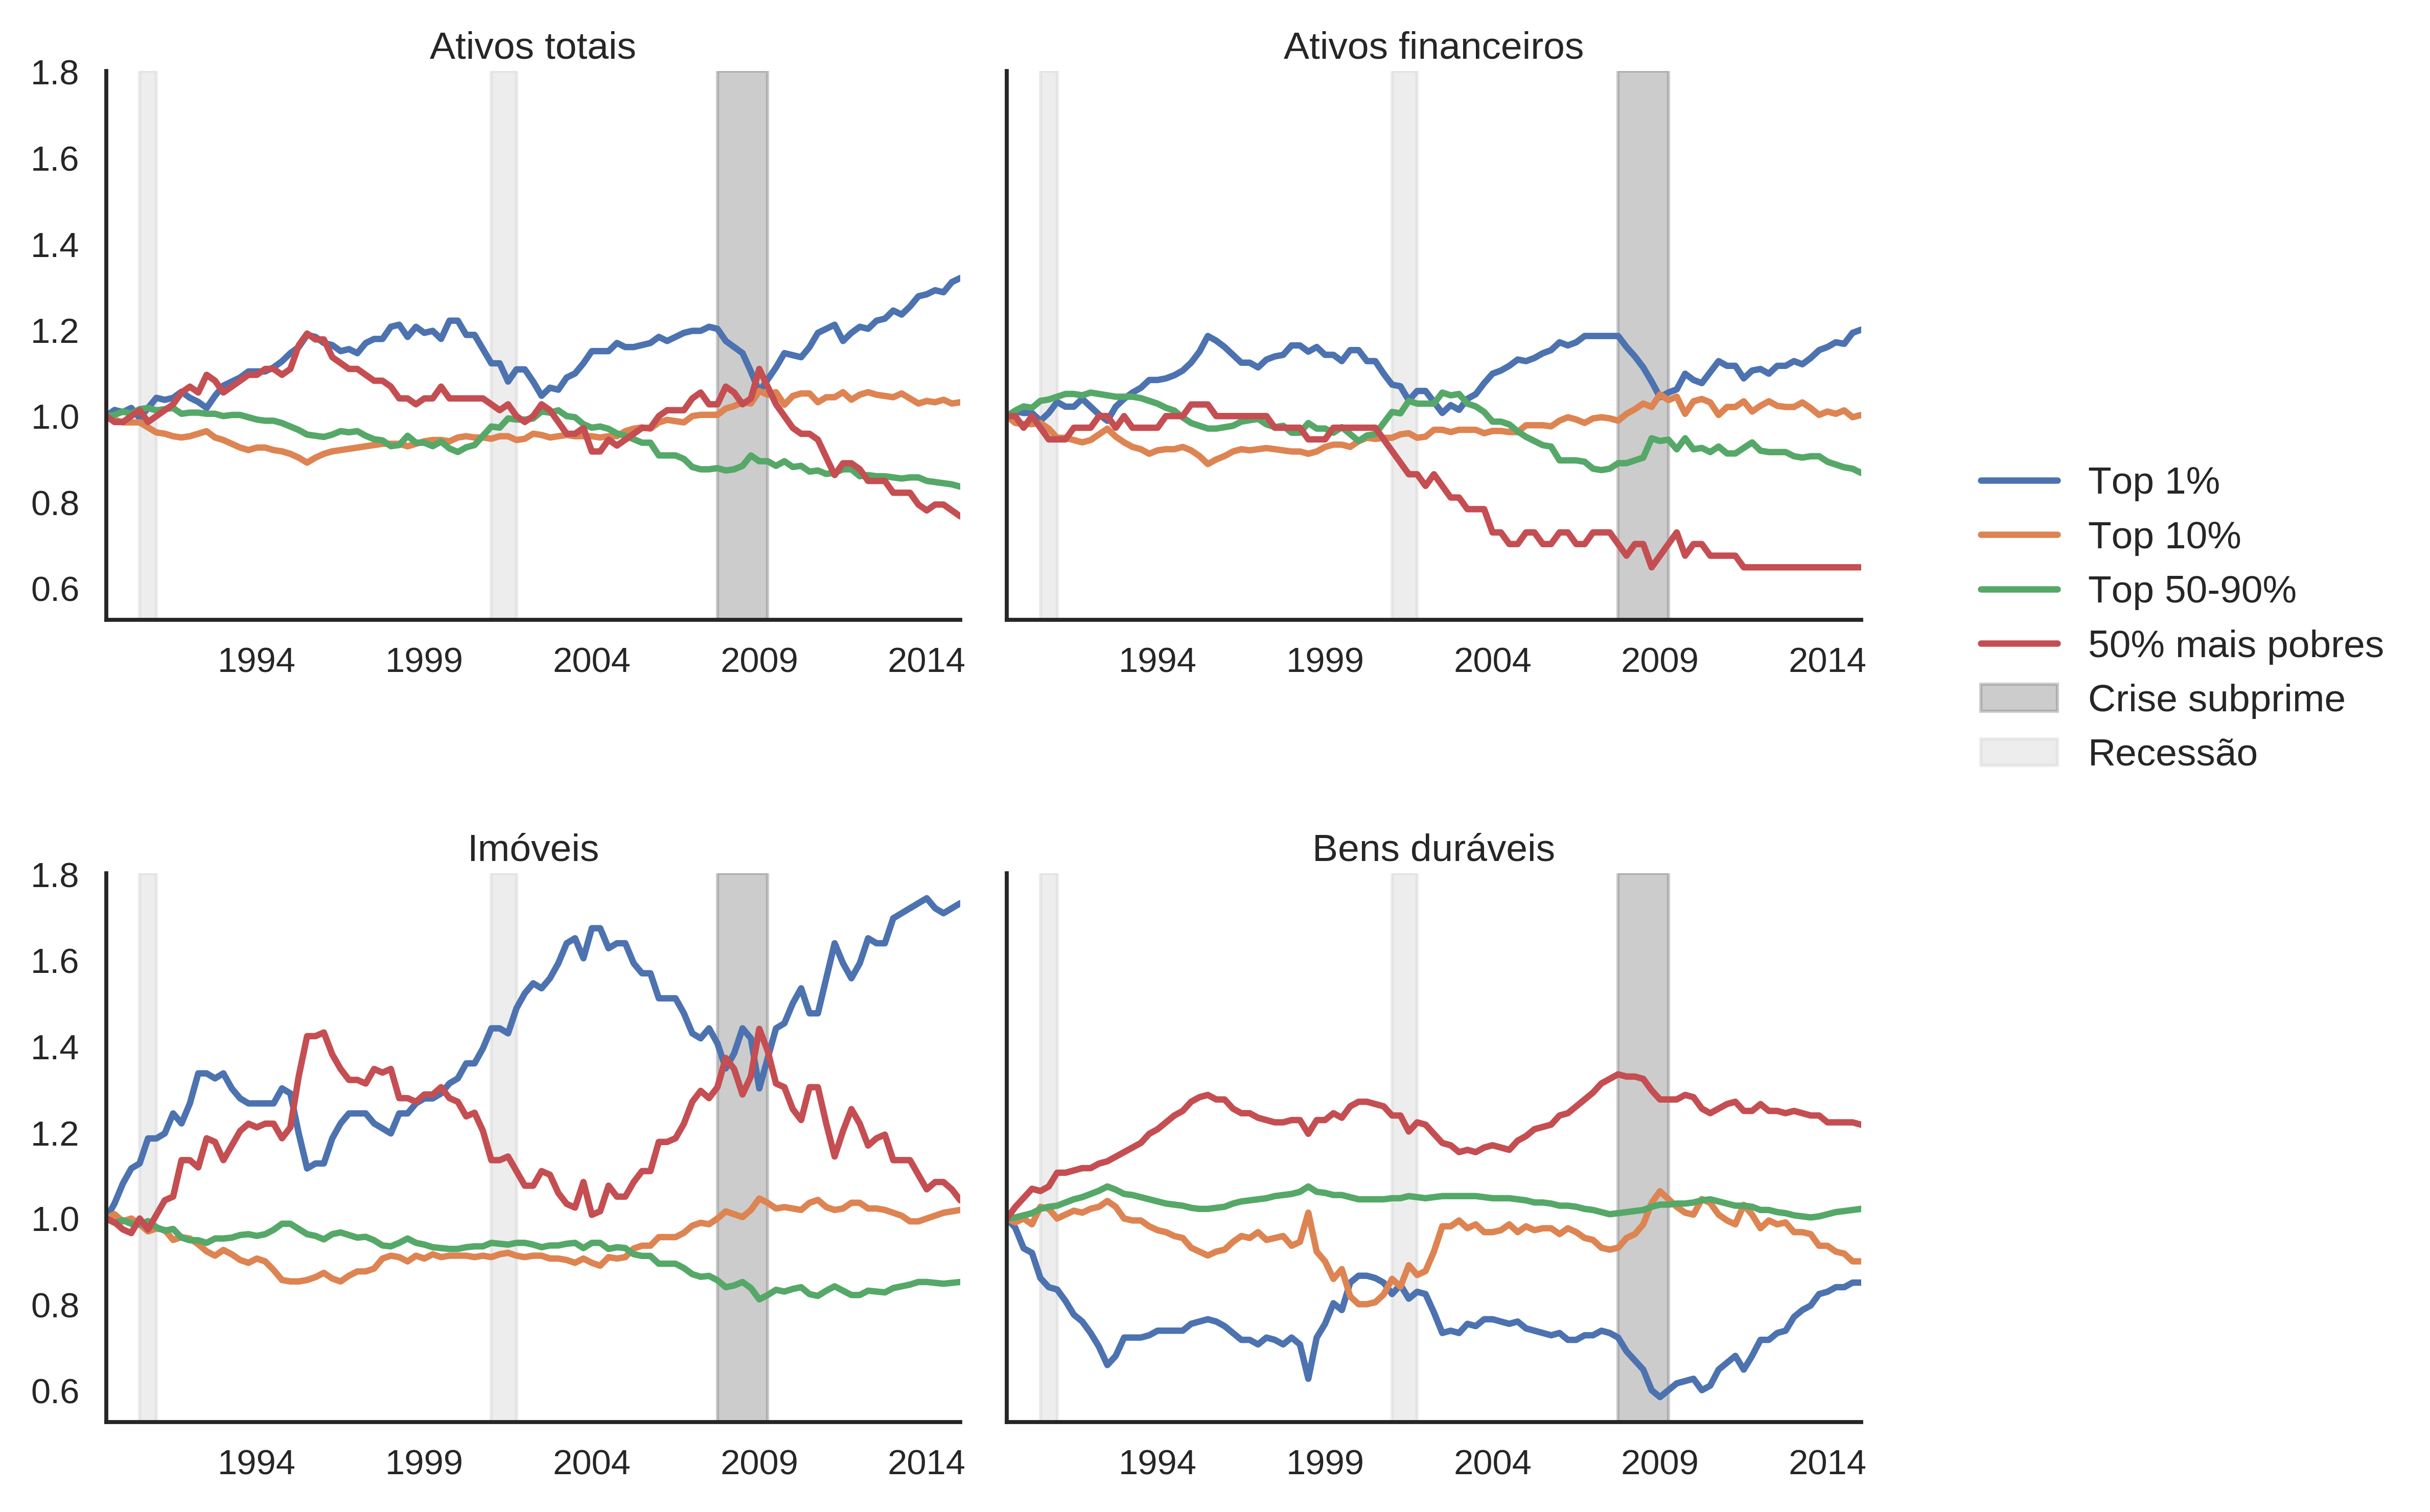
\includegraphics[width=\textwidth]{../../Dados/Fatos_Estilizados/figs/Distribuicao_Ativos.png}
	\caption*{\textbf{Fonte:} \textcite{us_census_bureau_characteristics_2017}, Elaboração própria}
\end{figure}

Os passivos (gráfico \ref{FigDistPassivos}), por sua vez, apresentam uma dinâmica semelhante entre si, ou seja, a participação nos empréstimos e nas hipotecas  é bastante similar ao longo do período analisado.
Argumenta-se aqui que tal resultado decorre da permissividade institucional americana.
De acordo com \textcite{teixeira_uma_2011}, os imóveis são uma das formas de riqueza mais comuns entre as famílias norte-americanas, servindo de colateral para tomada de crédito. A forma de ``realizar'' o ganho de capital com a bolha imobiliária que ocorreu no período, sem precisar liquidar os imóveis, era justamente ampliando o endividamento à medida que o colateral (\textit{i.e.} imóveis) aumentava de valor \cite{teixeira_crescimento_2015}. 


\begin{figure}[H]
	\centering
	\caption{Evolução de passivos por percentil de riqueza (1989/07=1)}
	\label{FigDistPassivos}
	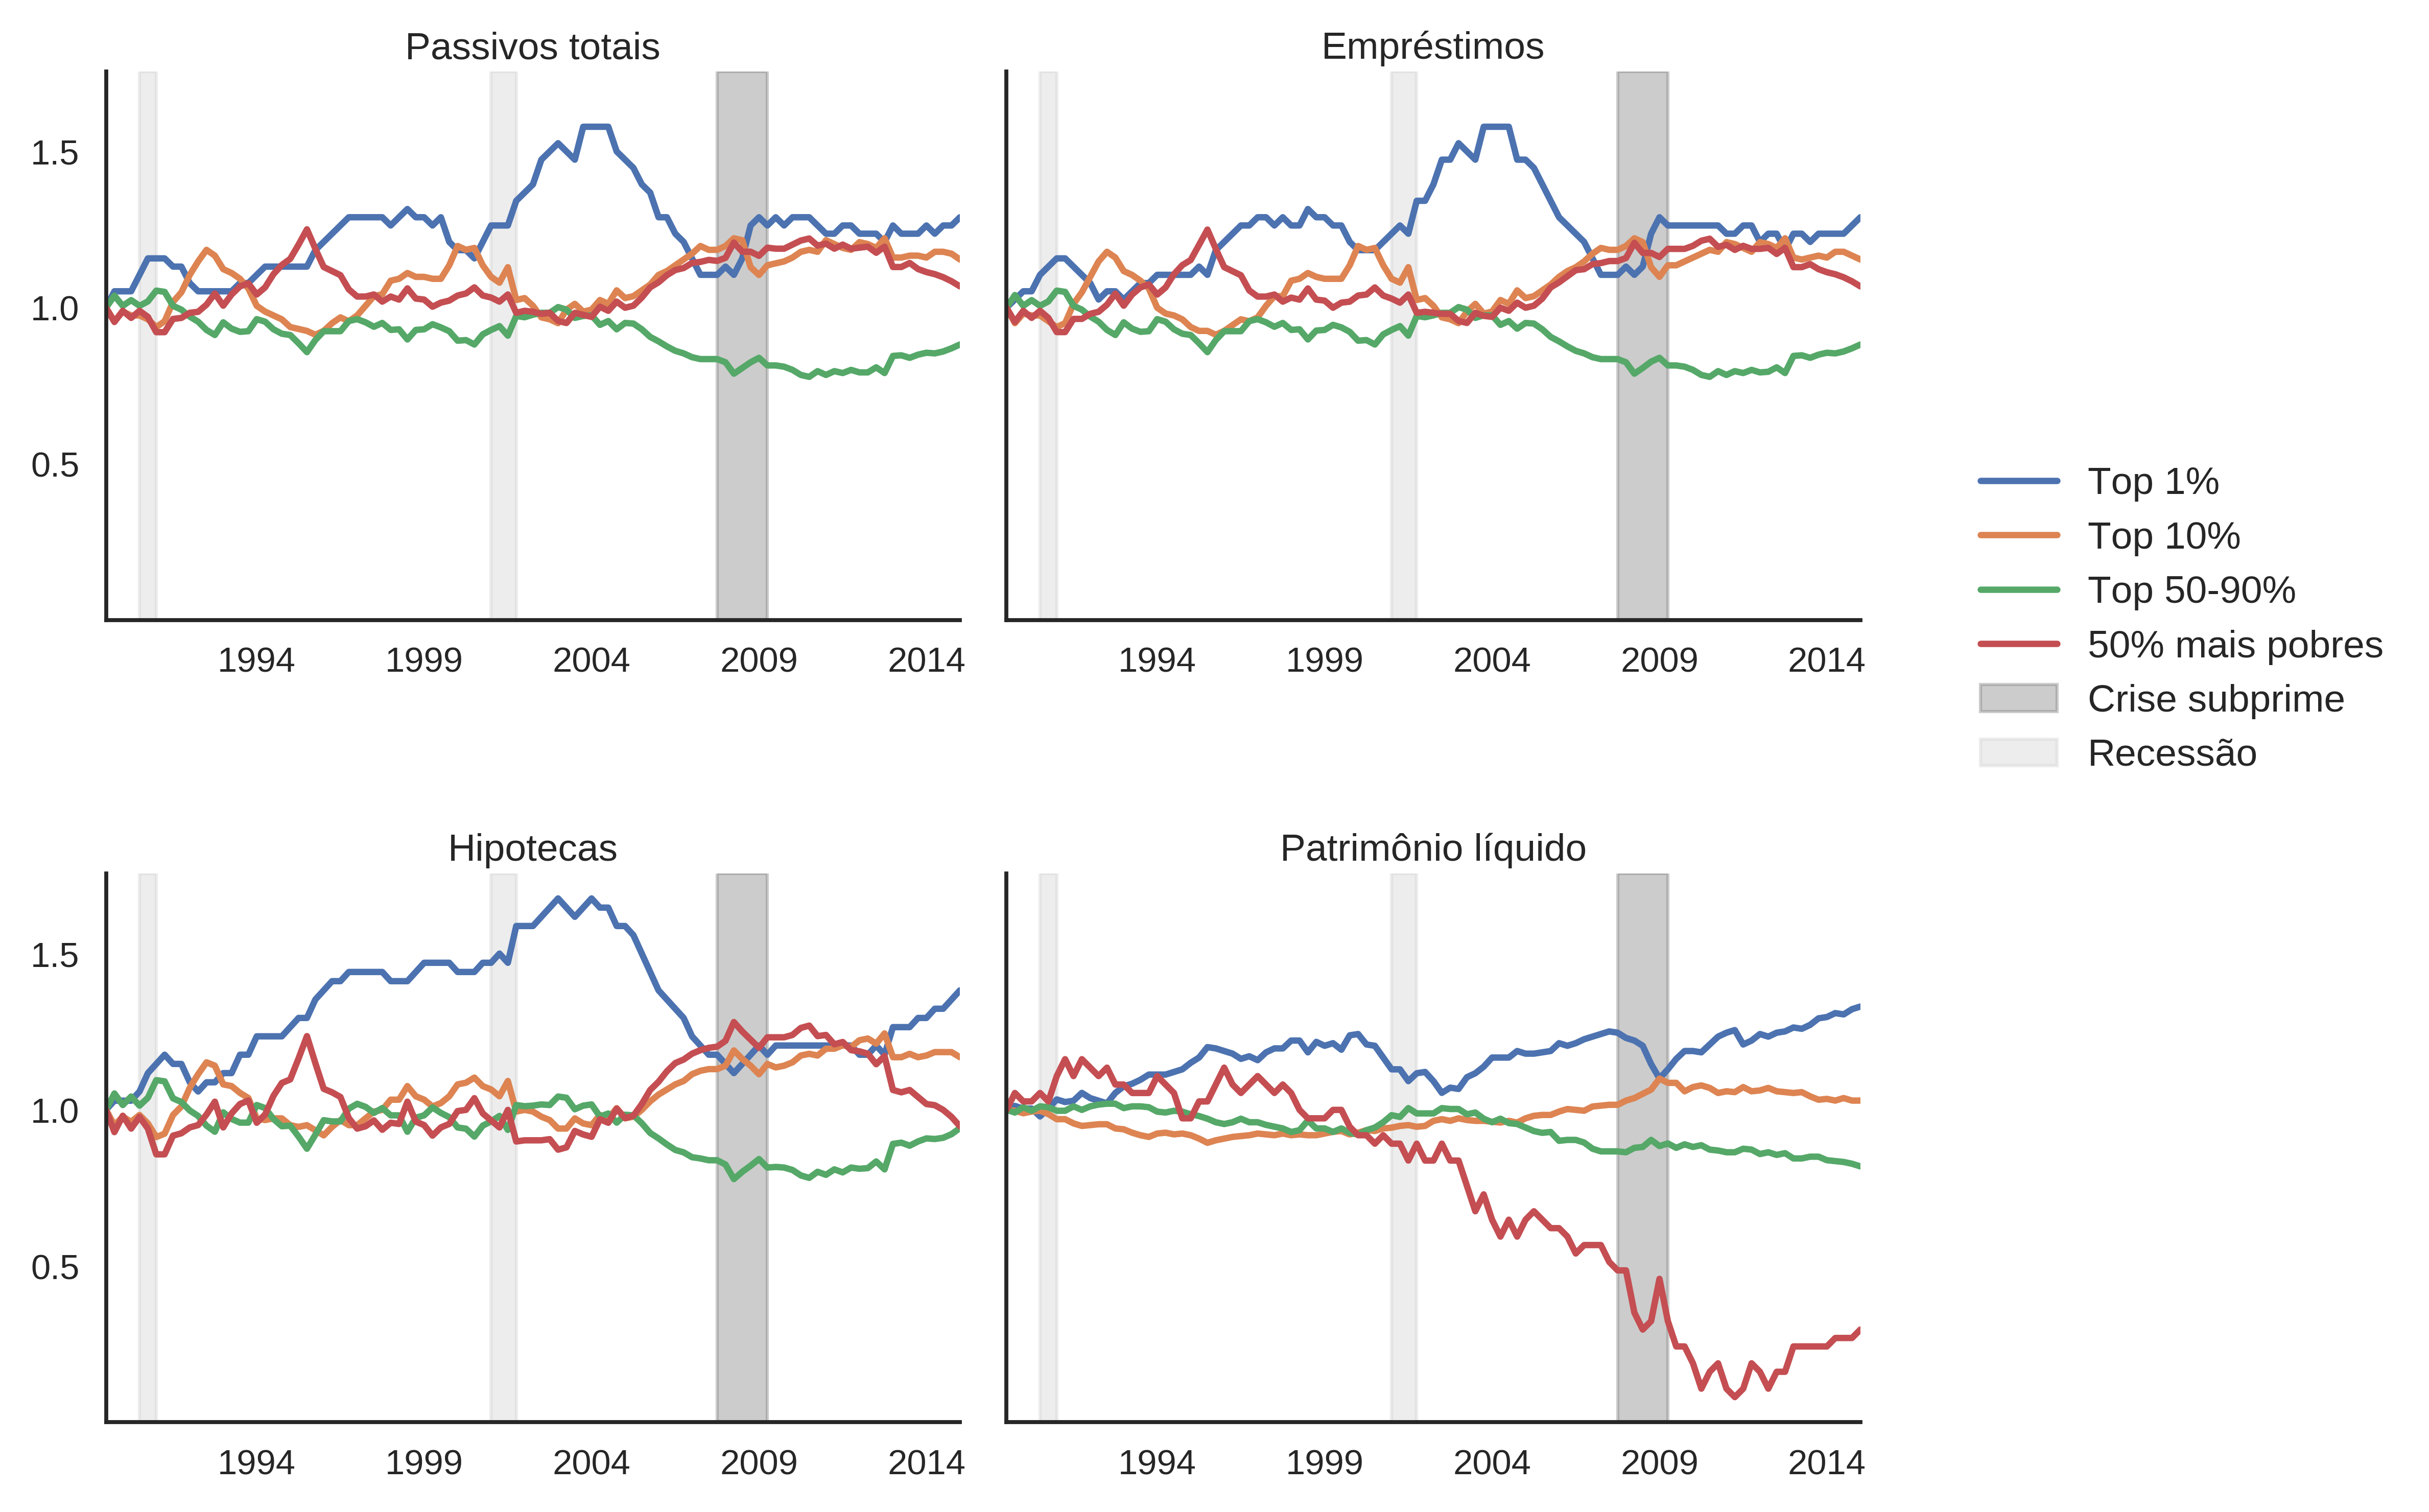
\includegraphics[width=\textwidth]{../../Dados/Fatos_Estilizados/figs/Distribuicao_Passivos.png}
	\caption*{\textbf{Fonte:} \textcite{us_census_bureau_characteristics_2017}, Elaboração própria}
\end{figure}


Como consequência, observa-se uma dinâmica gêmea (ver gráfico \ref{FigDividaPreco}) entre endividamento das famílias e preço dos imóveis que, por sua vez, permitia a ampliação do consumo --- sobretudo das famílias mais pobres --- mesmo com a estagnação salarial do período.
Tal especificidade institucional teve algumas implicações sobre a dinâmica macroeconômica que precisam ser melhor analisadas.
A primeira delas é o descolamento entre ativos e passivos no decorrer da crise financeira de 2008.
Esta separação decorre tanto do esgotamento da bolha dos imóveis (pós-2005) que fez com que os tais ativos desvalorizassem quanto da insensibilidade dos compromissos financeiros das famílias (\textit{i.e.} dívida) a queda do preço dos imóveis.
Em outras palavras, os imóveis (ativo) tem valor de mercado enquanto a dívida (passivo) tem um valor contratual sendo assim, o patrimônio líquido das famílias cai com o instaurar da crise.
A segunda implicação --- resultante da conjugação dos movimentos anteriores --- é a redução acentuada do patrimônio líquido das famílias mais pobres em termos absolutos e relativos (painel inferior direito do gráfico \ref{FigDistPassivos}).
%Em resumo, a estagnação dos salários somada às inovações financeiras que permitiram ampliação do consumo por meio de ampliação no colateral das famílias associado a elevação do preços dos imóveis resultaram em uma substituição dos salários por dívida \cite{barba_rising_2009}.


\begin{figure}[H]
	\centering
	\caption{Dinâmica do endividamento das famílias e do preço dos imóveis (jan/2000=100)}
	\label{FigDividaPreco}
	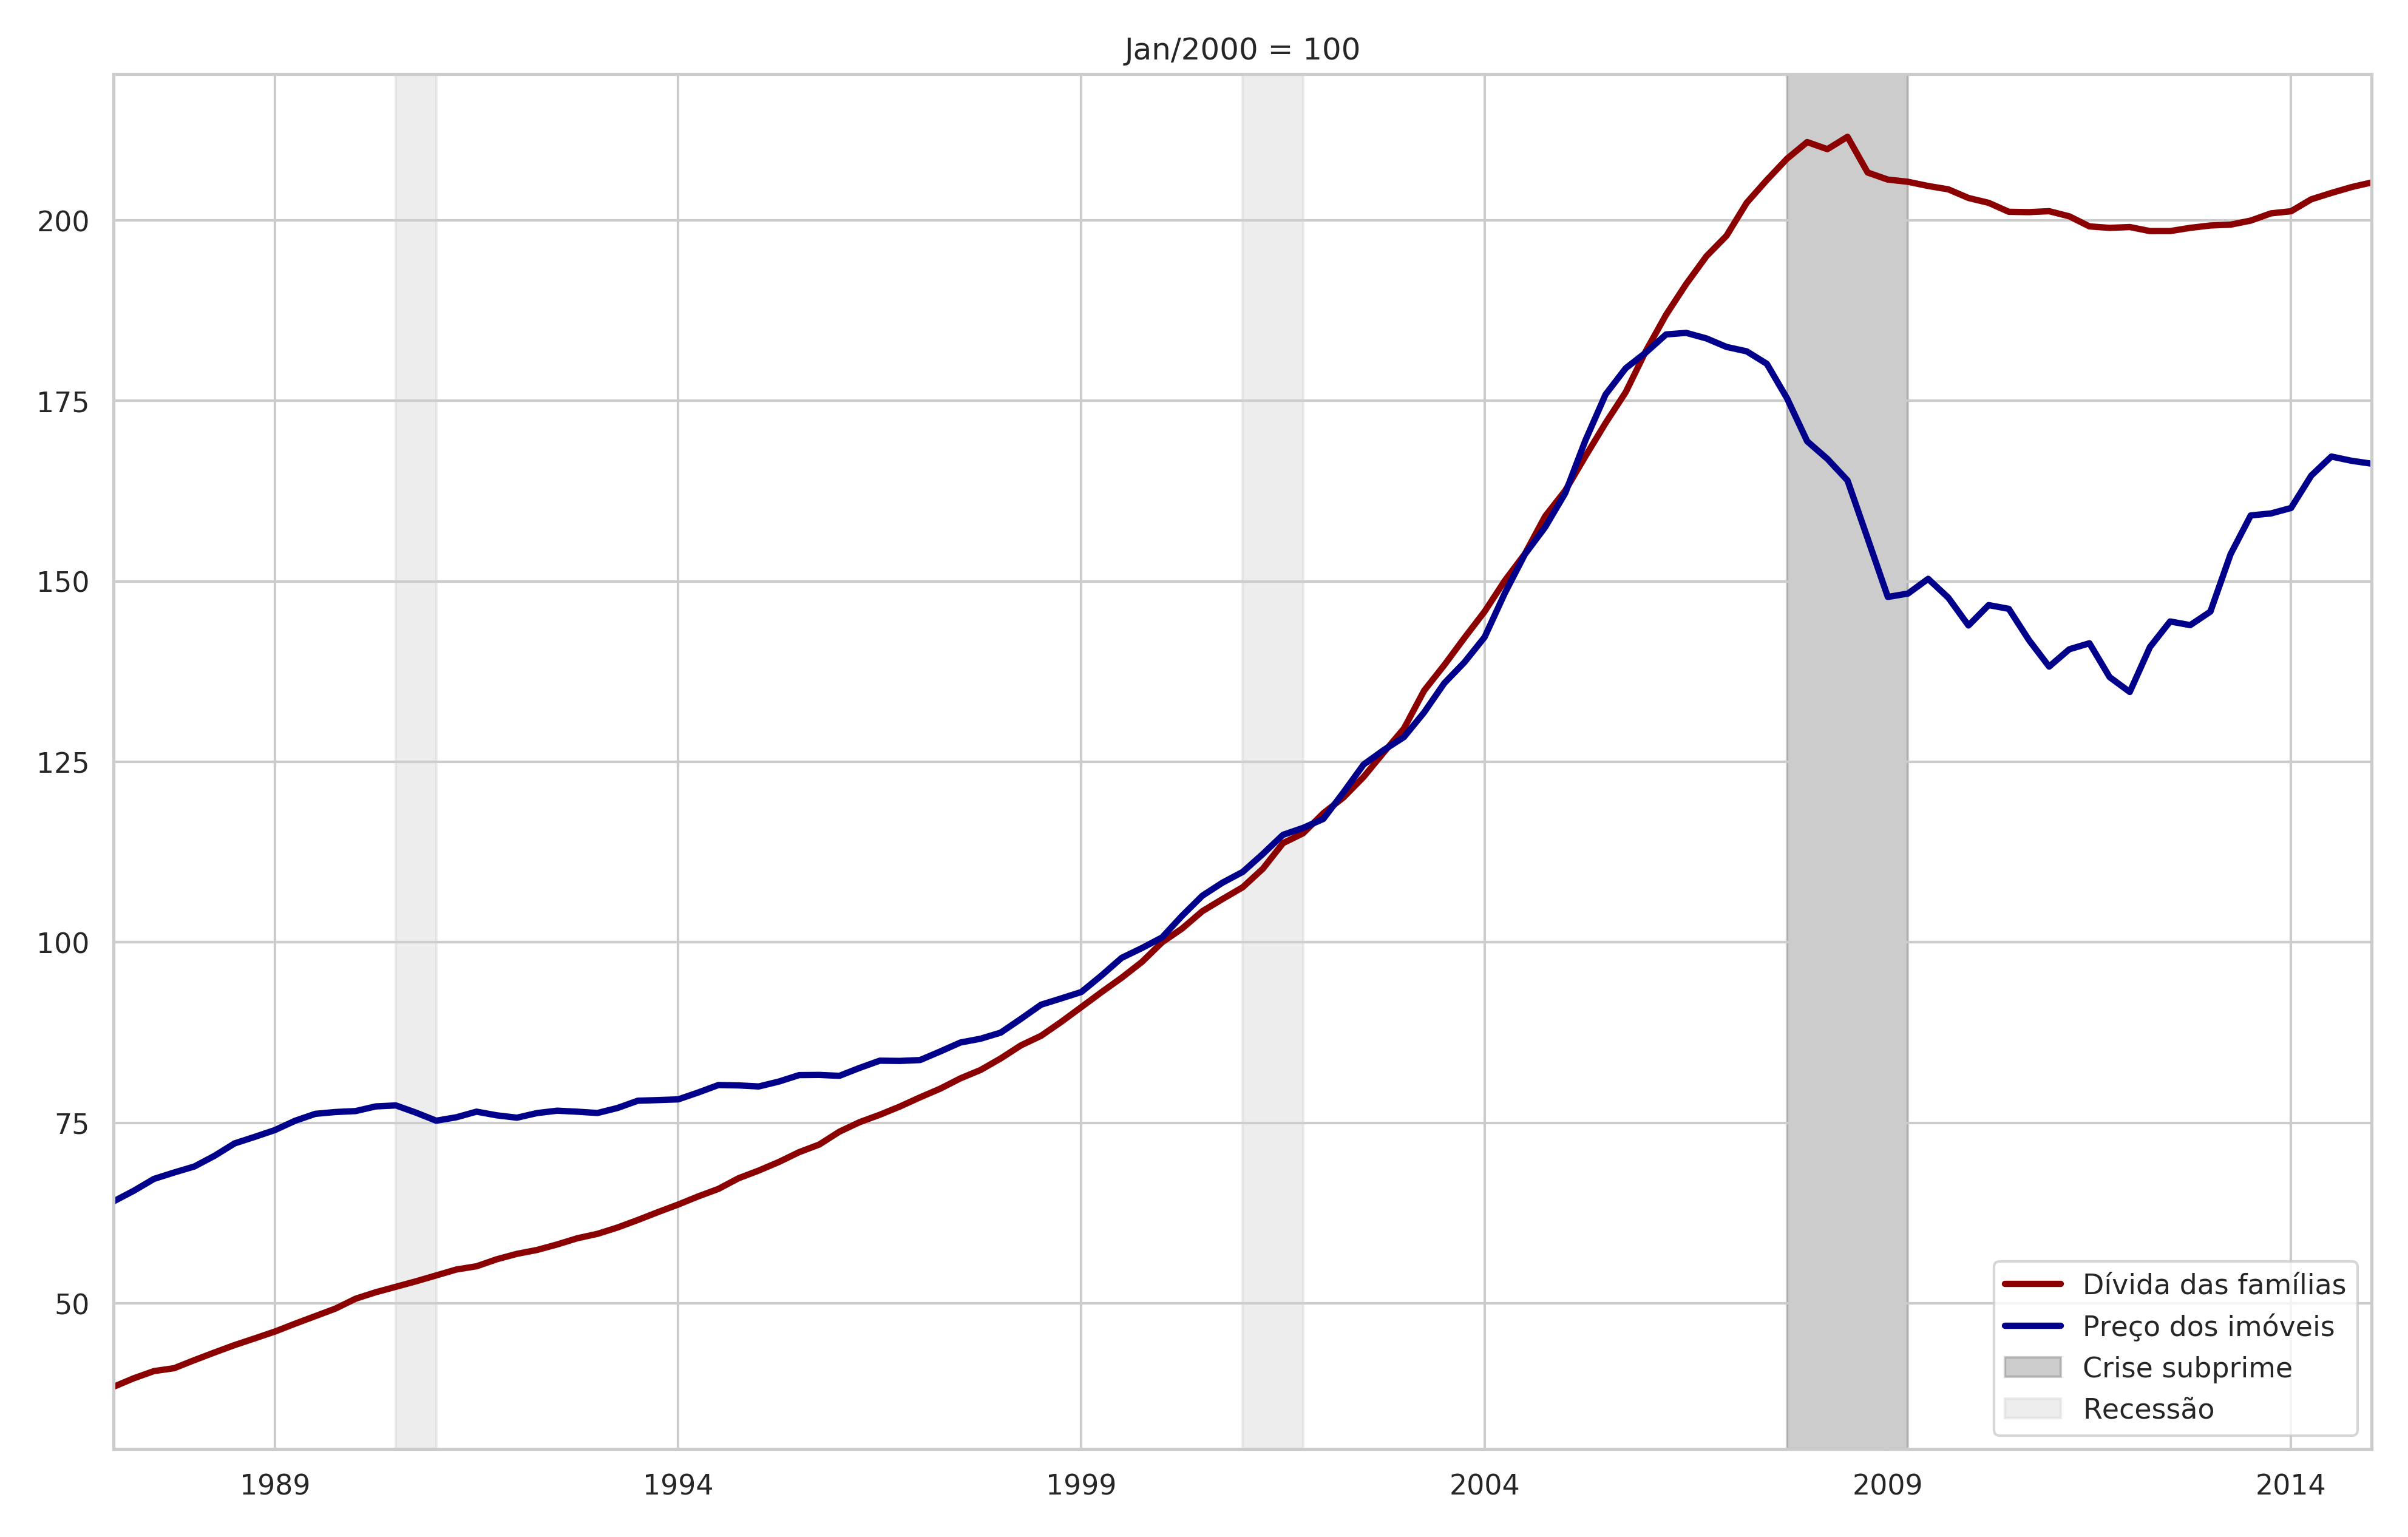
\includegraphics[width=\textwidth]{../../Dados/Fatos_Estilizados/figs/Divida_PrecoImoveis.png}
	\caption*{\textbf{Fonte:} U.S. Bureau of Economic Analisys, elaboração própria}
\end{figure}

%\begin{figure}[H]
%	\centering
%	\caption{Comprometimento da renda das famílias com o pagamento de juros (jan/1980 = 100)}
%	\label{FigServDiv}
%	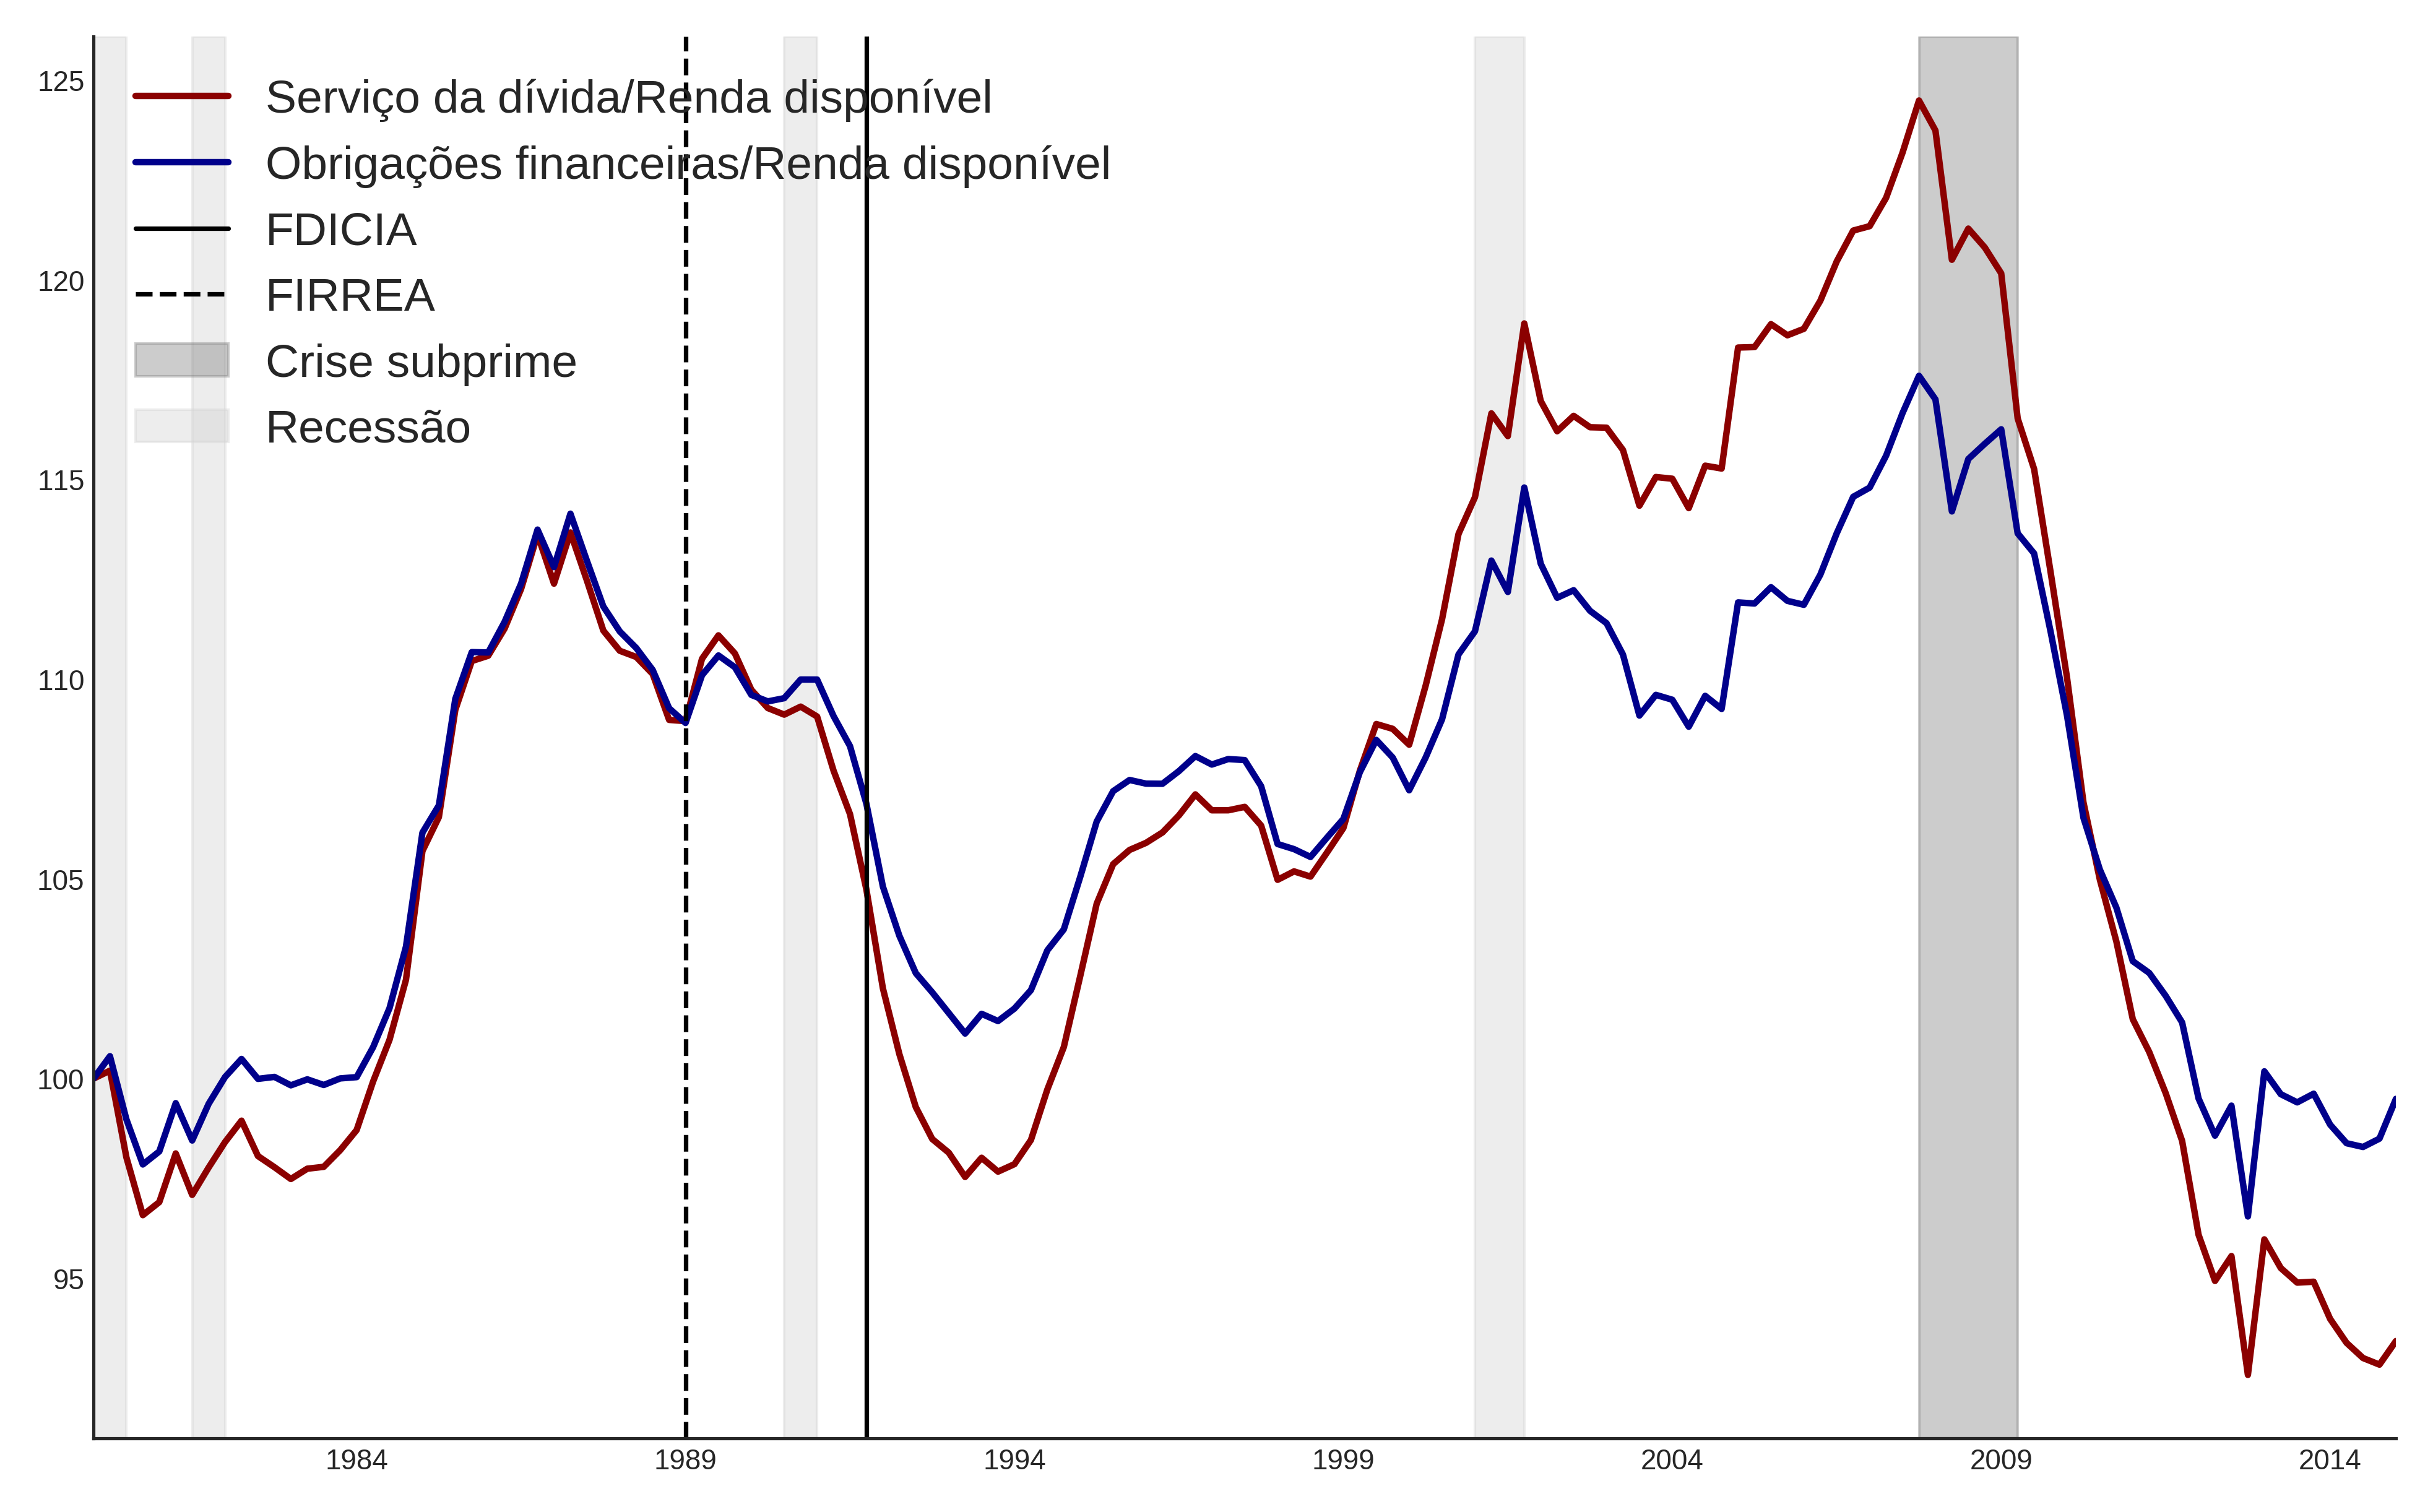
\includegraphics[width=\textwidth]{../../Dados/Fatos_Estilizados/figs/Serv_Divida.png}
%	\caption*{\textbf{Fonte:} U.S. Bureau of Economic Analisys, elaboração própria}
%\end{figure}


Existe também outra dimensão relevante que a literatura não dá a devida atenção: popularização dos imóveis primários\footnote{
	Em linhas gerais, um imóvel primário é aquele que o proprietário tem acesso regular e, no caso de possuir mais de um imóvel (secundário), é aquele que usufrui a maior parte do tempo ao longo do ano \cite{us_census_bureau_characteristics_2017}.
}.
A ampliação do acesso às residências pode ser visualizada no gráfico \ref{FigConcentracao} em que estão apresentadas as curvas de concentração\footnote{Em linhas gerais, curvas de concentração são elaboradas a partir da ordenação acumulada de duas variáveis distintas. No gráfico \ref{FigConcentracao}, ordenou-se os domicílios por riqueza no eixo horizontal enquanto o eixo vertical é ordenado pelos imóveis (primário e secundário) para então acumular ambos os eixos. Vale notar que a curva de Lorenz é um tipo específico de curva de concentração em que o eixo vertical apresenta a proporção acumulada da renda e proporção acumulada da população no eixo horizontal (ambos ordenados pela renda). Além disso, as curvas de concentração --- diferentemente da curva de Lorenz --- são não-decrescentes, podendo ultrapassar a linha de perfeita igualdade.
} de 1989 a 2010 por diferentes tipos de imóveis (primários e secundários).
%TODO Descrição dos imóveis primários e secundários
A partir destas curvas é possível avaliar quão concentrado é certo tipo de ativo comparando-o com a linha de perfeita igualdade\footnote{Quão mais acima e a esquerda da curva de Lorenz, menos concentrado/mais progressivo o ativo em questão está/é enquanto uma curva mais a direita e abaixo indica o oposto.
Neste caso, um ponto acima desta linha indica que o ativo em questão (neste caso, imóveis) é distribuído a favor dos estratos mais pobres da riqueza.
Além disso, a distribuição deste ativo contribuirá para a redução da desigualdade quanto mais inclinada for a curva de concentração na região dos mais pobres.
}.
Dito isso, uma breve inspeção deste gráfico revela que os anos que antecederam a Grande Recessão foram caracterizados pela desconcentração dos imóveis primários, ou seja, estratos mais pobres da população passaram a deter uma parcela acumulada maior deste tipo de imóvel.
Uma vez que as residências primárias dizem respeito àquelas que são utilizadas para fins não necessariamente especulativos, verifica-se uma elevação generalizada da demanda por imóveis enquanto moradia e não enquanto ativos (ver também gráfico \ref{FigDistAtivos}).
%IMÓVEIS PRIMÁRIOS POR QUE SÃO ÚTEIS E SECUNDÁRIOS PELA ESPECULAÇÃO
O mesmo não pode ser dito sobre os imóveis secundários\footnote{
	De acordo com o \textit{Survey of Construction} \cite{us_census_bureau_characteristics_2017}, os imóveis secundários são aqueles em que: (i) os proprietários residem parte do ano apenas; (ii) está ao menos 50 milhas do imóvel primário e; (iii) não pode estar sujeito a um contrato de aluguel.
} cujo movimento de concentração/distribuição não é tão demarcado quanto no caso anterior.
Além disso, uma vez que este tipo de imóvel não é destinado ao uso regular de seu proprietário, uma maior distribuição deste ativo sugere uma ampliação da demanda por imóveis na expectativa de ganhos de capital\footnote{
	Como pontuado no corpo do texto, esta aumento da demanda por imóveis secundários \textit{pode} indicar --- mas não se restringe a --- aumento por motivos especulativos. Uma casa de férias ou para aluguel, por exemplo, são usos não-especulativos de uma residência secundária.
	De todo modo, argumenta-se que há relação entre imóveis secundários e especulação.
}\footnote{Outro elemento que chama atenção no gráfico \ref{FigConcentracao} é que as famílias mais ricas não são as principais detentoras deste tipo de riqueza uma vez que acumulam menos da metade destes imóveis ao longo do período analisado.}.




%TODO Citar Survey

\begin{figure}[H]
	\centering
	\caption{Curva de concentração por tipos de imóveis}
	\label{FigConcentracao}
	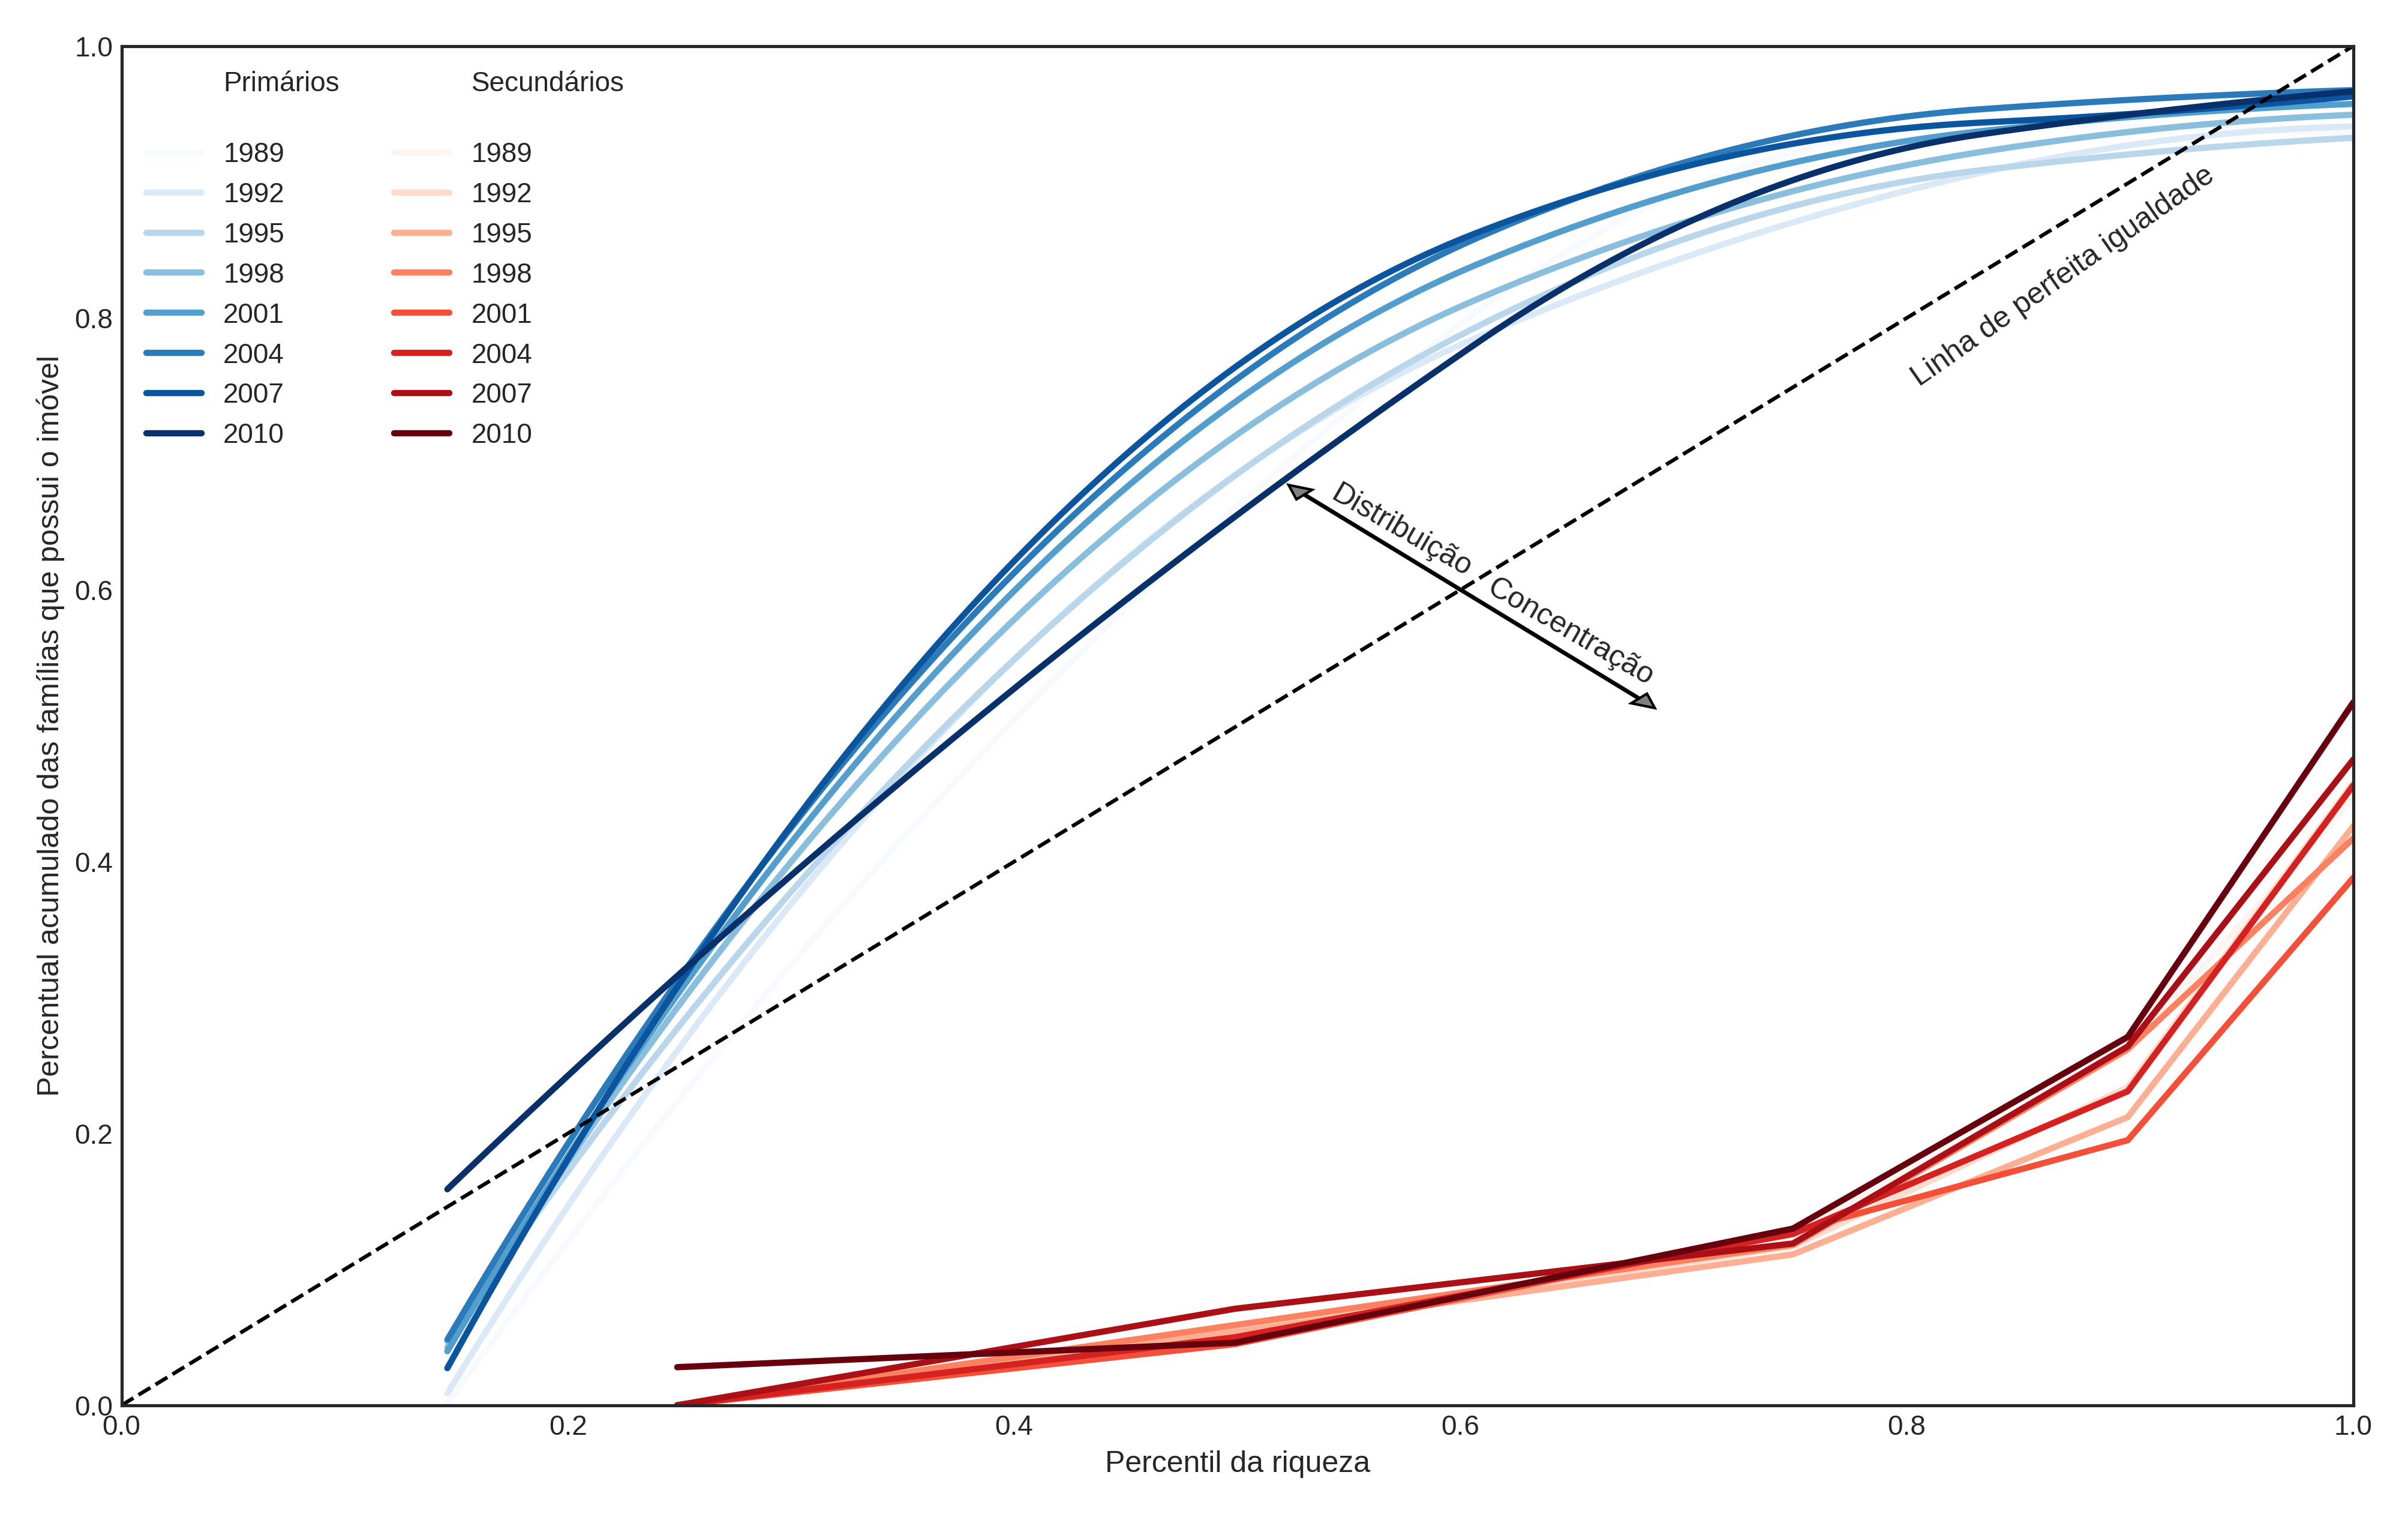
\includegraphics[width=\textwidth]{../../Dados/Fatos_Estilizados/figs/Concentracao_Imoveis.png}
	\caption*{\textbf{Fonte:} \textcite{us_census_bureau_characteristics_2017}, Elaboração própria}
\end{figure}
Por fim, partindo da hipótese apresentada no capítulo anterior (ver equação \ref{tx_Propria}) de que o investimento residencial possui um componente de longo prazo (popularização dos imóveis, por exemplo) e outro de médio prazo (especulação), argumenta-se que a relevância do aumento generalizado da participação dos imóveis
está associado  ao maior acesso ao crédito imobiliário --- sobretudo entre os estratos de renda mais baixos --- decorrente da desregulamentação financeira.
%Sendo assim, uma vez esgotada a bolha de ativos, os impactos são maiores que na ausência desta ``popularização residencial''.
%Isso somado a deterioração do patrimônio líquido das famílias mais pobres bem como maior comprometimento da renda disponível com o pagamento de juros (gráfico \ref{FigServDiv}) contribuiu para o delongamento da retomada desta crise mais recente.

%%%%%%%%%%%% RESUMO PARA OS CHOQUES
Em resumo, pontuou-se a relevância do investimento residencial para dinâmica macroeconômica.
Aliado a isso, outros fatos estilizados foram apresentados e que serão levados adiante nos choques do capítulo \ref{CapModelo} , são eles:
	(i) ampliação da demanda por imóveis por motivos especulativos (via aumento do coeficiente $\phi_1$);
	(ii) aumento da demanda por imóveis associada às mudanças demográficas (via aumento do coefieinte $\phi_0$);
	(iii) redução da participação dos salários na renda (por meio de alterações no \textit{wage-share}, $\omega$)
	e;  
	(iv) maior comprometimento da renda das famílias com pagamento de juros da dívida (via aumento da taxa de juros).
Apresentados estes fatos estilizados, cabe a seção seguinte investigar como a literatura econométrica tem tratado o investimento residencial em termos macroeconômicos.

%Teixeira e a taxa própria

\subsection{Investimento residencial nos modelos macroeconométricos}\label{RevEmpirica}

Compreendida a importância do investimento residencial para a dinâmica macroeconômica americana, faz-se necessária uma investigação dos determinantes deste gastos de acordo com a literatura econométrica e este é o objetivo desta seção. 
No entanto, dado o objeto desta pesquisa, destaca-se aqueles trabalhos que enfatizam a importância da construção de novos imóveis para o ciclo econômico para além da contribuição de \textcite{leamer_housing_2007}.


É importante pontuar que nos anos que procederam a crise do mercado imobiliário, verificou-se um crescente interesse nas implicações macroeconômicas do investimento residencial. Inspecionando modelos DSGE que incluem investimento residencial, \textcite{iacoviello_housing_2010} conclui que um melhor entendimento dos impactos deste gasto se faz necessária para a compreensão das flutuações macroeconômicas. Outros estudos, por sua vez, têm enfatizado o efeito riqueza sobre o consumo via valorização dos imóveis e indicam tais canais de transmissão são mais incidentes, em ordem, sobre Estados Unidos e Grã Bretanha mas mais brandos no caso francês e alemão \cites{sastre_assessment_2010}{chauvin_wealth_2010}{bassanetti_effects_2010}{arrondel_housing_2010}. 
\textcite{alvarez_does_2010}, por sua vez, concluem que tal tipo de investimento antecede o ciclo econômico para o caso de espanhol e resultados semelhantes podem ser encontrados para França, Espanha  e Itália enquanto na Alemanha esta dinâmica é distinta \cites{ferrara_common_2010}{ferrara_cyclical_2010}{ferrara_common_2010}\footnote{\textcite{alhowaish_causality_2015}, por outro lado, destaca que o investimento em infra-estrutura é induzido pelo setor petrolífero no caso da Arábia Saudita. Apesar de contrapor \textcite{green_follow_1997}  e \textcite{leamer_housing_2007}, tal resultado não é comparável uma vez que não é feita a devida distinção entre os gastos em construção civil feitos pelo governo e investimento residencial propriamente dito. Resultados semelhantes são obtidos por \textcite{ofori_testing_2003} em que investimento residencial também é somado ao investimento em infraestrutura.}. 

Um estudo que se sobressai é o de \textcite{arestis_residential_2015} em que é estendida a contribuição de \textcite{poterba_tax_1984} por meio de um modelo ARDL para 17 países da OCDE. Dentre as conclusões, destaca-se a importância da renda disponível como principal determinante do investimento residencial para os países em questão.  A implicação deste resultado, no entanto, questionaria a possibilidade de tratar o investimento residencial enquanto um gasto autônomo e, portanto, comprometeria a análise a partir do supermultiplicador sraffiano. Porém, tal resultado não é estatisticamente significante para o caso norte-americano em que o preço dos imóveis bem como o acesso ao crédito são os principais determinantes desse gasto e, desse modo, reaviva a discussão para a presente investigação.


Outro estudo recente é o de \textcite{huang_is_2018} em que os autores testam ambas as hipóteses aventadas por Leamer a despeito do investimento residencial (predição e causalidade). Para isso, estimam um modelo VAR estrutural (SVAR) com transformada \textit{wavelets} para os países da OCDE\footnote{
	Além de testar se a construção de novos imóveis antecipa movimentos no ciclo econômico, os autores também testam os canais de transmissão da política monetária em quatro frentes: (i) teoria neoclásica do investimento residencial; (ii) efeito riqueza do preço dos imóveis sobre o consumo por meio de um modelo de ciclo de vida; (iii) efeito do colateral sobre o balanço patrimonial das famílias e consumo; (iv) efeito do colateral sobre o balanço patrimonial dos bancos e oferta de crédito.}.  
Os autores concluem que o investimento residencial não é um mero canal de transmissão da política monetária e que possui efeitos temporalmente distintos sobre o ciclo econômico. No curto prazo, a construção de novos imóveis tem maior capacidade preditiva enquanto o preço dos imóveis tem maior influência no longo prazo\footnote{Adicionalmente, \textcite{huang_is_2018} também concluem que a capacidade preditiva do investimento residencial é maior quanto maior a parcela deste gasto no produto.}. A razão desta distinção, argumentam, é que a transmissão da política monetária via o canal da riqueza é mais proeminente no longo prazo enquanto os canais de crédito e de colateral são mais presentes no curto prazo. Já no que diz respeito a relação causal estabelecida por \textcite{leamer_housing_2007}, afirmam que os resultados não são conclusivos para todos os países diante da heterogeneidade institucional observada\footnote{
	No entanto, os autores afirmam que para a maioria dos países do G7 o investimento residencial é ao menos capaz de amplificar o ciclo econômico.}, mas ainda é valida para os Estados Unidos\footnote{
	Apenas para ilustrar a dimensão da importância do investimento residencial para o ciclo econômio norte-americano, \textcite{huang_is_2018} utilizam este pais como critério de comparação.}.
Apesar dos resultados não conclusivos sobre as flutuações, concluem que as variáveis associadas ao investimento residencial (preço dos imóveis, taxa real de juros das hipotecas --- deflacionada pelo índice de preços --- e \textit{spread} bancário) lideram o crescimento econômico.

Apesar de significativo, o estudo  de \textcite{huang_is_2018} reportado acima é centrado em determinantes do lado da oferta, sobretudo custos de produção (\textit{user costs}) e, portanto, não é compatível com a agenda da demanda efetiva.
Uma alternativa é o de \textcite{gauger_residential_2003} em que os autores investigam os efeitos da desregulamentação das instituições depositárias ao longo da década de 80. Para tanto, estimam um VEC entre agregados monetários (M2), taxas de juros (de curto e longo prazo) PIB e investimento residencial.
Dentre as conclusões, os autores destacam que a taxa de juros de longo prazo passa a contribuir cada vez mais para variância do investimento residencial:
\begin{citacao}
	\textit{The findings for the two interest rates give valuable information to evaluate results in
	other studies. Results here suggest that use of a short-term FFR and post-deregulation data
	may lead to conclusions that `interest rate shocks are much less important after
	deregulation.' The fuller slate of evidence here indicates that interest rate shocks remain
	important post-deregulation; however, now it is the long-term rate shocks that carry more
	information for housing sector movements} \cite[p.~346]{gauger_residential_2003}
\end{citacao}

As conclusões deste estudo são bastante relevantes para a presente pesquisa pelas seguintes razões: 
	(i) explicita --- tal como no supermultiplicador --- relações de longo prazo entre investimento residencial e outras variáveis macroeconômicas e; 
	(ii) destaca a importância de mudanças institucionais para o mercado imobiliário.
Uma forma de visualizar o item (ii) é por meio da figura \ref{FigCreditoFDICIA} em que estão assinaladas algumas das reformas ocorridas ao longo dos anos 80 e início dos 90 por conta da crise dos \textit{Savings and Loans}  (FIRREA e FDICIA respectivamente).
Dentre as consequências destas mudanças, destaca-se a subsequênte eliminação da restrição de crédito que permitiu a expansão do financiamento do investimento residencial nos períodos seguintes.

RODAPÉ FFDICIA

\begin{figure}[htb]
	\centering
	\caption{Concessão de crédito às famílias e hipotecas (Taxa de crescimento)}
	\label{FigCreditoFDICIA}
	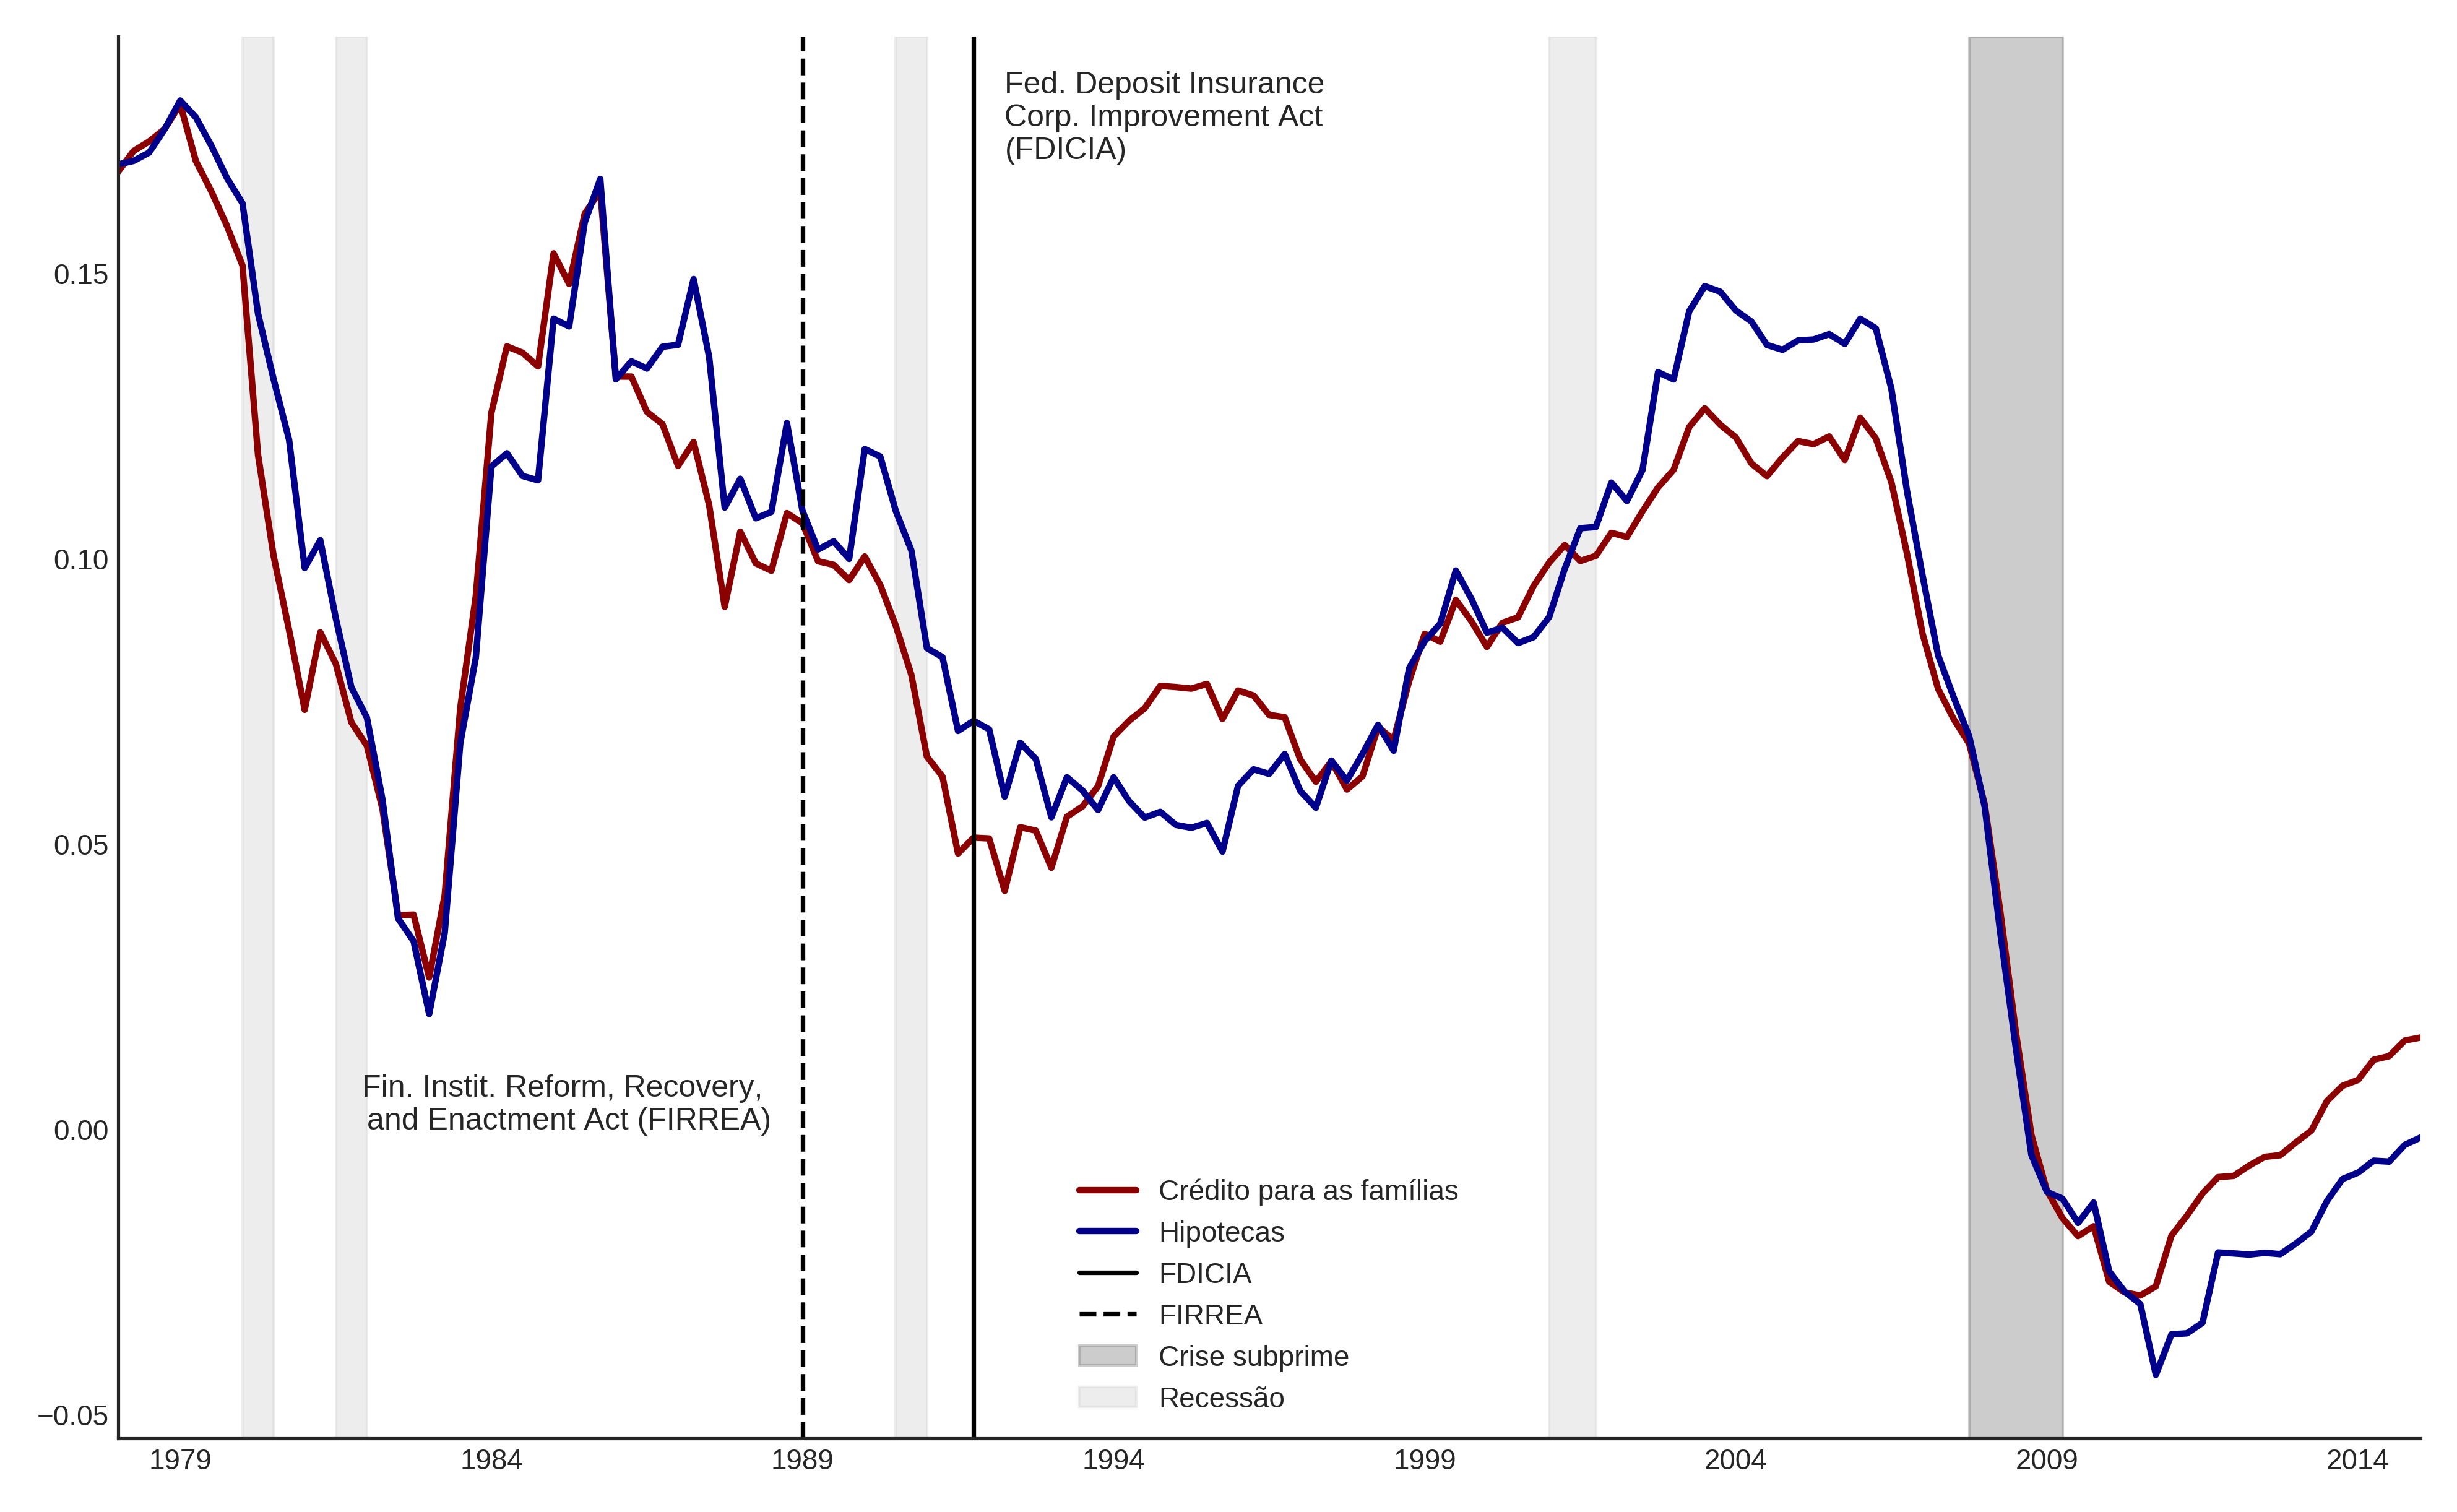
\includegraphics[width=\textwidth]{../../Dados/Fatos_Estilizados/figs/FDICIA.png}
	\caption*{\textbf{Fonte:} U.S. Bureau of Economic Analisys, elaboração própria}
\end{figure}
	
Apesar de \textcite{gauger_residential_2003} concluirem que a taxa de juros (de longo prazo) continua sendo relevante para explicar o investimento residencial, conclui-se que o procedimento destes autores não é o mais adequado por tratarem os juros como endógeno e determinado por agregados monetários. Sendo assim, seguir tal proposta incorre-se em uma inconsistência com a teoria heterodoxa em que as taxas de juros é uma variável exógena determinada por meio de um processo decisório pelo autoridade monetária de modo que a oferta de moeda é endógena \cite[p.~230--256]{lavoie_post-keynesian_2015}.

Uma forma de incluir o investimento residencial na macroeconomia da demanda efetiva sem incorrer nestes problemas é a da já mencionada taxa própria de juros dos imóveis desenvolvida por \textcite{teixeira_crescimento_2015}. A partir deste constructo teórico, é possível explicitar o custo real para se construir imóveis em termos de imóveis de modo a captar tanto o custo do endividamento quanto ganhos de capital.
Para tanto, deflaciona-se a taxa de juros hipotecárias --- diferentemente de \textcite[p.~143--146]{fair_macroeconometric_2013} --- pela inflação de imóveis tal como na equação EQUAÇÃO.


Para evidenciar esta relação, o gráfico \ref{gZ_Propria} ilustra como  este deflacionamento é mais adequado para captar a dinâmica do investimento residencial.
Destaca-se também que em momentos de especulação (\textit{i.e.} bolha de ativos, neste caso, imóveis) é a inflação destes ativos que domina a dinâmica da taxa própria \cite[p.~53]{teixeira_crescimento_2015}. Sendo assim, quanto menor esta taxa maiores serão os ganhos de capital (em imóveis) por se especular com imóveis.
Tal dinâmica é evidenciada no gráfico \ref{gZ_Propria} em que a taxa própria se reduziu progressivamente ao longo do \textit{boom} imobiliário (2002-5).
Apesar de lançar luz sobre algumas relações relevantes --- ausentes em \textcite{godley_seven_1999} --- esta proposição não foi avaliada por meio da estimação de um modelo macroeconométrico. Desse modo, a seção seguinte pretende verificar a capacidade explicativa desta alternativa.


%ESTES ESTUDOS INDICAM A RELEVÂNCIA DO INVESTIMENTO RESIDENCIAL PARA A DINÂMICA.


%TODO Alterar imagem


\begin{figure}[H]
	\centering
	\caption{Taxa real e própria de juros dos imóveis x investimento residencial}
	\label{gZ_Propria}
	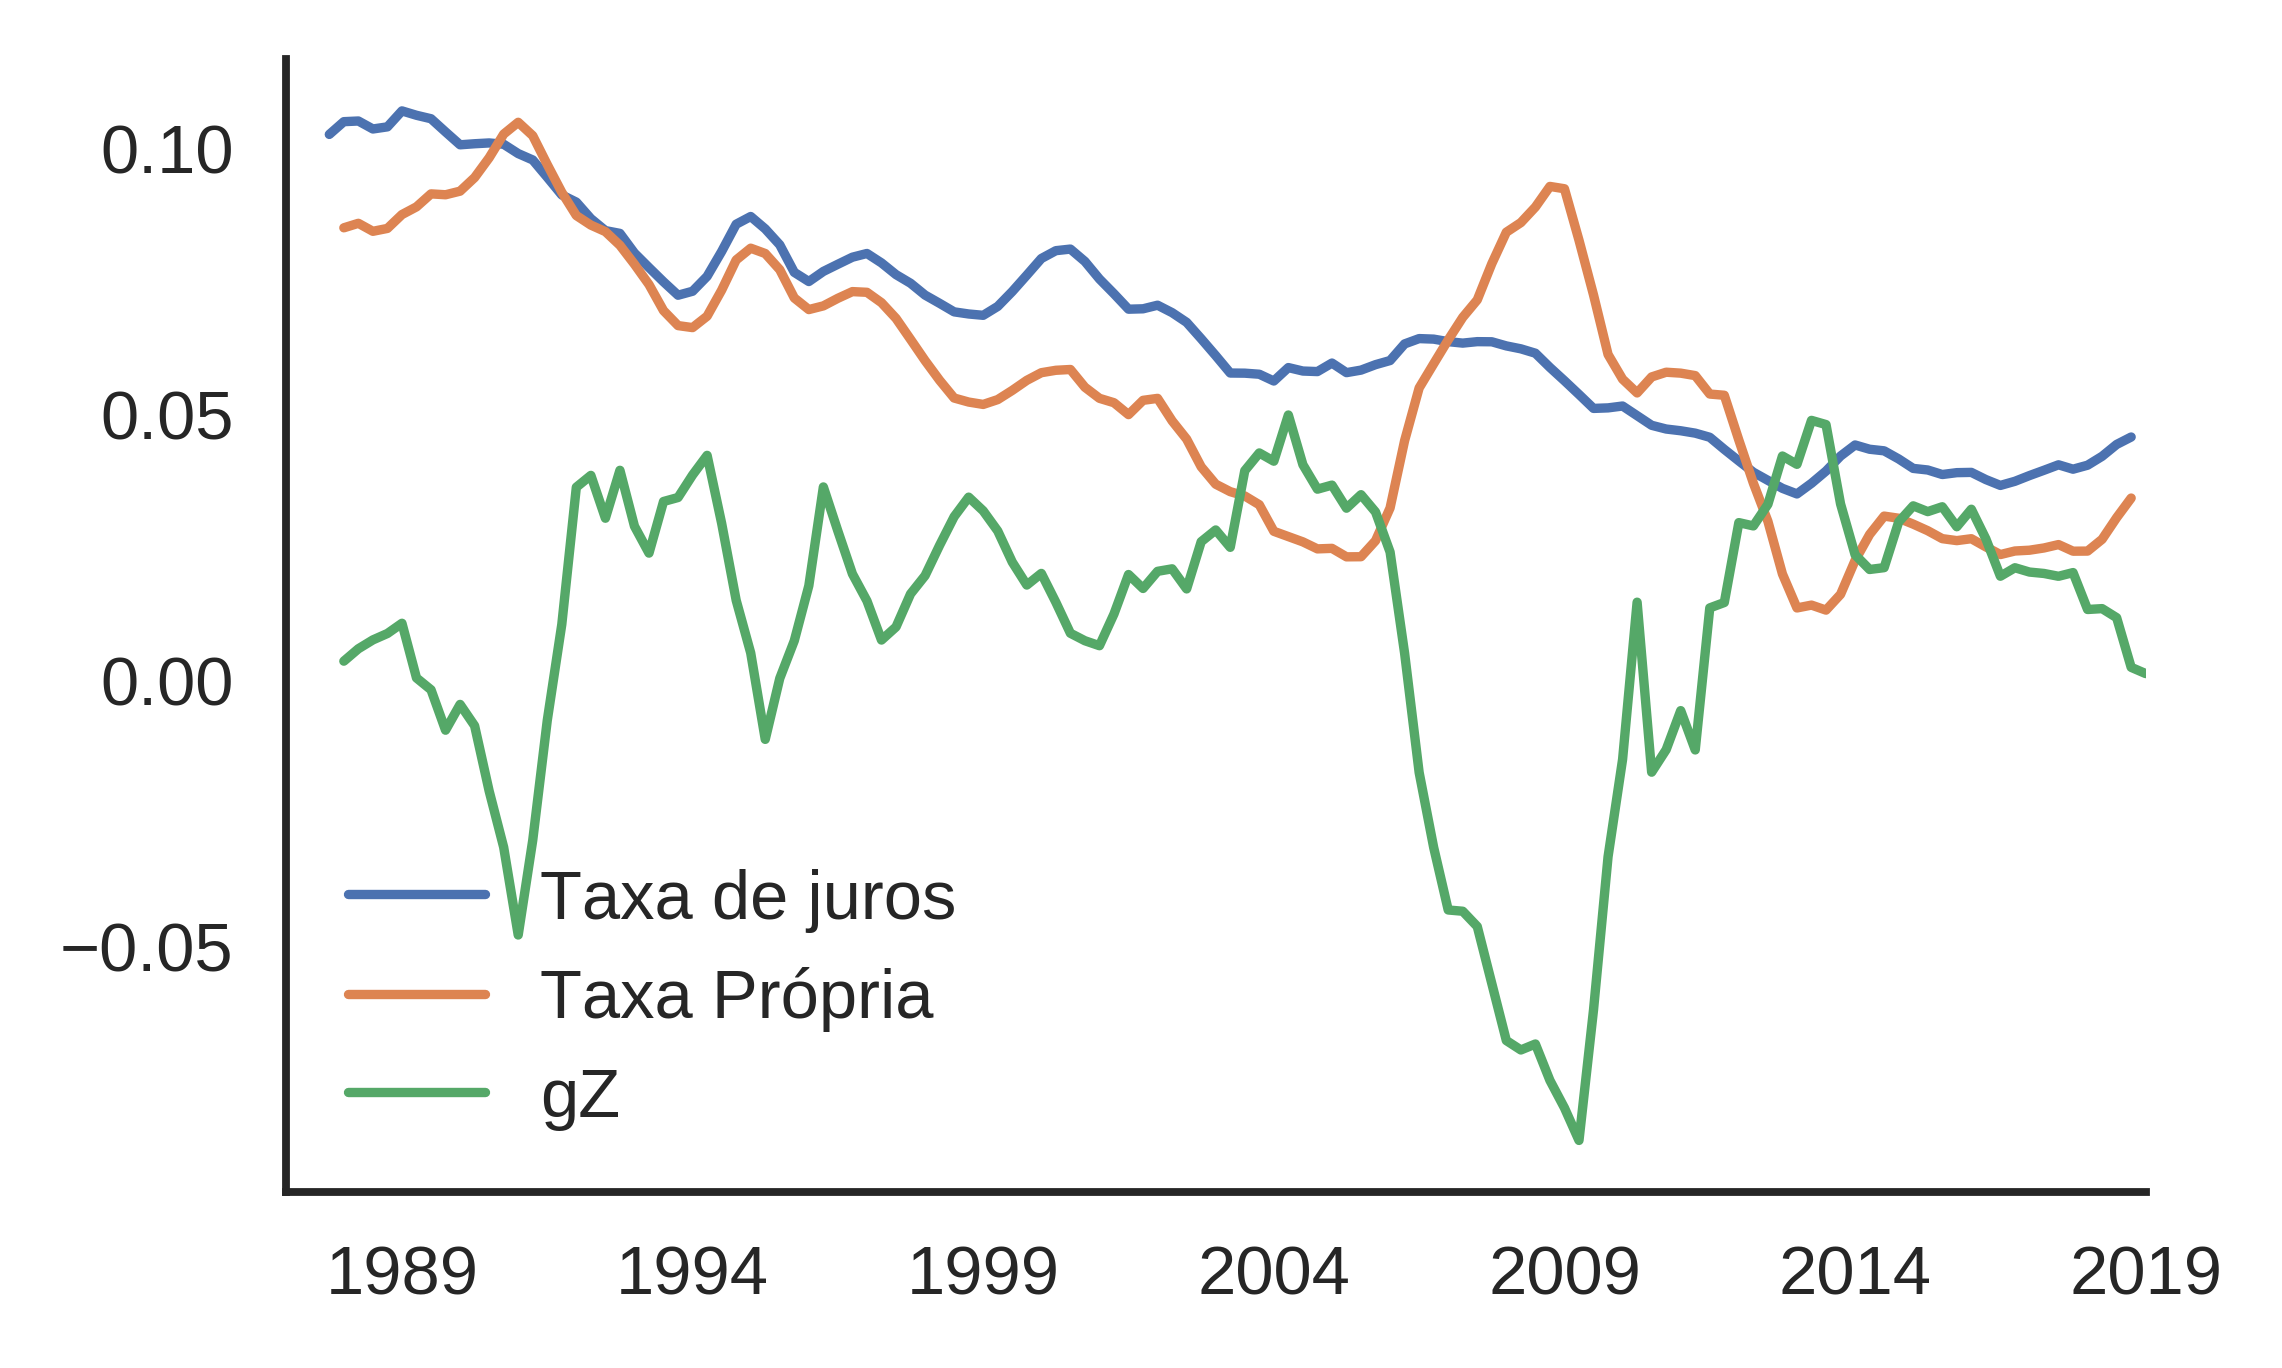
\includegraphics[width=0.75\textwidth]{../../Dados/Fatos_Estilizados/figs/TxPropria_Investo.png}
	\caption*{\textbf{Fonte:} U.S. Bureau of Economic Analysis, elaboração própria}
\end{figure}






\section{Modelo}
\label{SecModelo}

Por padrão, as variáveis exógenas, $j$ diga-se, serão indicadas por $\overline{j}$ enquanto os parâmetros serão denotados por letras gregas. Além disso, as equações não numeradas são apenas etapas algébricas enquanto as numeradas estão presentes nas rotinas utilizadas. Por fim, vale a menção de que os códigos deste modelo estão disponíveis e foram escritos em \textit{python} com o uso do pacote \textit{pysolve3} que foi desenvolvido ao longo desta pesquisa.

\paragraph*{Equações gerais}
O produto é determinado pelo estoque de capital criador de capacidade assim como pelo trabalho homogêneo. Além disso, supõe-se temporariamente que não estão presentes inflação de bens bem como depreciação\footnote{A ausência de depreciação é meramente simplificadora e será incluída nas versões futuras deste modelo. Vale mencionar que um dos objetivos desta pesquisa é incorporar e analisar os impactos da inflação de ativos.}.  Diferentemente de \textcite{nikiforos_utilization_2016} e \textcite{dutt_observations_2018}, supõe-se que estão ausentes retornos crescentes de escala e progresso tecnológico.

Por se tratar de uma economia sem relações externas e sem governo, o produto determinado pelos componentes da demanda ($Y$) é a soma do consumo ($C$) e investimento das famílias ($Ih$) e das firmas ($If$) em que apenas este último é criador de capacidade produtiva ao setor privado:

\begin{equation}
\label{_Y}
    Y = [C + Ih] + [If]
\end{equation}
da equação acima é possível deduzir o investimento total ($It$):

\begin{equation}
\label{_It}
    It = If + Ih
\end{equation}

Considerando uma função de produção \textit{à la} leontieff, o produto potencial ($Y_{FC}$) é determinado por:

$$
Y_{FC} = \min (Y_K, Y_L)
$$
em que $Y_K$ e $Y_L$ são respectivamente produto de plena capacidade e de pleno emprego definidos por:

$$
Y_K = \frac{1}{\overline v}K_{f_{-1}} \hspace{2.5cm} Y_L = \frac{1}{\overline b}L_{-1}
$$
com $v$ e $b$ sendo relações técnicas e $K_f$ e $L$ indicam respectivamente o estoque de capital criador de capacidade ao setor privado e  o trabalho. Tal como é convencional na literatura, supõe-se que o capital é escasso em relação ao trabalho. Nesses termos, o produto potencial é:

\begin{equation}
\label{_YFC}
    Y_{FC} = Y_K
\end{equation}
o que permite escrever o grau de utilização da capacidade ($u$):

$$
u = \frac{Y}{K_f}\cdot \overline v
$$

\begin{equation}
\label{_u}
    u = \frac{Y}{Y_{FC}}
\end{equation}
cuja forma em termos de crescimento equivale a
\begin{equation}
\label{Aux}
\tag{Aux.}
\dot u = (g - g_K)\cdot u_{t-1}
\end{equation}
em que $g_Y$ e $g_K$ são, respectivamente, a taxa de crescimento da demanda e da capacidade produtiva discutidas no capítulo teórico.


A razão pela qual o capital criador de capacidade se difere do estoque de capital total da economia ($K$) se dá pela inclusão do investimento residencial tão comumente ignorado pela literatura que, como pontuado pelo capítulo anterior, possui implicações importantes para a dinâmica da economia norte americana. Dito isso, o estoque de capital é dado por:

\begin{equation}
\label{_K}
    K = Kf + K_{H}
\end{equation}
em que $K_H$ refere ao acúmulo do investimento residencial. Seja $K_k$ a participação dos imóveis no estoque de capital total da economia:

\begin{equation}
\label{_tau}
K_k = \frac{K_H}{K}    
\end{equation}
é possível representar a equação \ref{_K} de forma alternativa:
$$
K = K_k\cdot K + (1-K_k)\cdot K
$$
que será utilizada para o desenvolvimento da solução analítica.

Neste modelo, tal como na tradição Kalekicana e Sraffiana, a distribuição funcional da renda é exógena. Para não recorrer à hipóteses a respeito da estrutura de mercado bem como da determinação de preços das firmas, impõe-se que:

\begin{equation}
    \omega = \overline{\omega} \Leftrightarrow \pi = 1 - \overline{\omega}
\end{equation}
em que $\omega$ e $\pi$ são respectivamente a participação dos salários e dos lucros na renda. O que permite escrever a massa de salários nos seguintes termos:

$$
\omega = \frac{W}{Y}
$$

\begin{equation}
\label{_W}
    W = \omega\cdot Y
\end{equation}

Por fim, cabe explicitar os ativos financeiros presentes no modelo e como são distribuídos entre os diferentes agentes institucionais. As famílias (denotadas pelo subíndice $h$) acumulam riqueza sob a forma de depósitos à vista ($M$) enquanto contraem empréstimos hipotecários ($MO$) para realizar investimento residencial que, no acumulado, é idêntico ao estoque de imóveis ($K_h$). 
%Além disso, tal como pontuado por \textcite{leamer_housing_2007}, possuem acesso a crédito ($N$) a depender do estoque de riqueza (imóveis neste caso) e é financiado por dívida ($L_h$)
As firmas (denotadas pelo subíndice $f$), por sua vez, financiam o investimento em parte por lucros retidos e o restante por empréstimo ($L_f$). Os bancos, portanto, criam crédito (\textit{ex nihilo}) para então recolher os depósitos, todos remunerados pelas respectivas taxas de juros. Com isso, é possível explicitar a matriz dos estoques:


\begin{table}[H]
\centering
\caption{Matriz dos estoques}
\begin{tabular}{lcccc}
\hline
\hline


                          & Famílias      & Firmas        & Bancos  &    $\sum$ \\ \hline

Depósitos & $+M$ & & $-M$ & 0\\
Empréstimos das firmas & &$-L_f$& $+L_f$ & 0\\
Hipotecas &$-MO$&  & $+MO$ & 0\\\hline
$\sum$ Riqueza financeira líquida &$V_h$&$V_f$&$V_b$& $0$\\\hline
Capital & &$+K_f$&  & $+K_f$\\
Imóveis &$+K_{HD}$& &   & $+K_{H}$\\\hline
$\sum$ Riqueza líquida total&$NW_h$&$NW_f$&$NW_b$& $+K$\\
\hline
\hline
\end{tabular}%
\caption*{\textbf{Fonte:} Elaboração própria}
\end{table}

Esta matriz além de mapear as relações entre os diferentes agentes institucionais de modo que não existam ``buracos negros'', permite explicitar as interelações entre lado real e financeiro \cite{dos_santos_revisiting_2010}. Resta explicitar como os fluxos determinam os estoques por meio da matriz de transações correntes e fluxo de fundos que, descritas as hipóteses e equações gerais, auxiliará na especificação de cada setor institucional:

\begin{table}[H]
\centering
\caption{Matriz de transações correntes e fluxo de fundos}
\resizebox{\textwidth}{!}{%
\begin{tabular}{lcccccc}
\hline
\hline
& \multicolumn{2}{c}{Famílias}
& \multicolumn{2}{c}{Firmas}                        
& Bancos       & Total    \\ \cline{2-3}\cline{4-5}
& 
Corrente & Capital & 
Corrente & Capital     & 
&        $\sum$ \\ 
Consumo                         &$-C$& & $+C$& & & 0\\
Investimento                    & & &$+If$&$-If$ & & 0\\
Investimento residencial        & &$-Ih$&$+Ih$& & & 0\\
\textbf{{[}Produto{]}}   & & &{[}$Y${]}& & & {[}$Y${]}\\
Salários                        &$+W$& &$-W$& & & 0\\
Lucros                      &$+FD$& &$-FT$&$+FU$& & 0\\
Juros (depósitos)         &$+r_m\cdot M_{-1}$& && &$-r_m\cdot M_{-1}$& 0\\
Juros (empréstimos)         && &$-r_l\cdot L_{f_{-1}}$& &$+r_l\cdot L_{-1}$& 0\\

Juros (hipotecas)         &$-r_{mo}\cdot MO_{-1}$& && &$+r_{mo}\cdot MO_{-1}$& 0\\\hline
\textbf{Subtotal}           &$+S_h$&$-I_h$& &$+NFW_f$&$+NFW_b$& 0\\\hline
Variação dos depósitos     &$-\Delta M$& & & &$+\Delta M$& 0\\
Variação das hipotecas     & &$+ \Delta MO$& & &$-\Delta MO$& 0\\
Variação dos empréstimos     & &&$+\Delta L_f$&$-\Delta L$& 0\\
\textbf{Total} & 0 & 0 & 0  & 0  & 0  & 0\\
\hline
\hline
\end{tabular}%
}
\caption*{\textbf{Fonte:} Elaboração própria}
\end{table}

\paragraph*{Firmas} Para produzir, as firmas encomendam bens de capital ($-If$ na conta de capital) e contratam os trabalhadores que são remunerados pela massa de salário de modo que os lucros brutos ($FT$) são determinados por:

\begin{equation}
    FT = Y - W
\end{equation}
Além disso, as firmas retêm uma parcela ($\gamma_F$) dos lucros líquidos de juros ($FU$) e distrubuem o restante para as famílias ($FD$):

\begin{equation}
    FU = \gamma_F\cdot (FT - r_l\cdot L_{f_{-1}})
\end{equation}
\begin{equation}
    FD = (1-\gamma_F)\cdot (FT - r_l\cdot L_{f_{-1}})
\end{equation}

Como sugerido pelo capítulo \ref{CapFatos} e seguindo a literatura do supermultiplicador sraffiano, supõe-se que o investimento das firmas é induzido pelo nível de demanda efetiva,
\begin{equation}
\label{_If}
    If = h\cdot Y
\end{equation}
em que $h$ é a propensão marginal à investir. Além disso, adota-se o princípio do ajuste do estoque de capital de modo que as firmas revisam seus planos de investimento de forma que o grau de utilização se ajuste ao normal ($u_N$):
\begin{equation}
\label{_h}
    \Delta h = h_{-1}\cdot \gamma_u\cdot (u - \overline{u}_N)
\end{equation}
em que o parâmetro $\gamma_u$ deve ser suficientemente pequeno para que este ajustamento seja lento e gradual. Contabilmente, o investimento das firmas determina o estoque de capital criador de capacidade produtiva:

\begin{equation}
    \Delta Kf = If
\end{equation}

Adicionalmente, as firmas financiam o investimento que excede os lucros retidos por meio de empréstimos dos bancos remunerados à taxa $\overline r_l$ definida exogenamente. Por hipótese, supõe-se que consigam se financiar sem restrições de forma que a demanda/oferta por crédito para as firmas é definida por:

\begin{equation}
    \Delta L_f = If - FU
\end{equation}

Por fim, como pode ser verificado pela tabela de transações correntes, o saldo financeiro líquido das firmas ($NFW_f$) é:

\begin{equation}
    NFW_f = FU - If
\end{equation}
em que as firmas são devedoras líquidas se o investimento for maior que os lucros retidos. Por definição, se um dos setores é deficitário ao menos um precisa ser superavitário para que a soma dos saldos financeiros líquidos seja nula enquanto a soma do estoque de riqueza financeira seja igual ao estoque de capital da economia. A matriz dos estoques, por sua vez, fornece a riqueza líquida das firmas ($NW_f$):
\begin{equation}
    NW_f = K_f - L_f
\end{equation}

\paragraph*{Bancos} Tal como grande parte da literatura SFC, os bancos neste modelo não desempenham um papel ativo e atuam como intermediadores financeiros. No entanto, isso não implica que existe uma precedência dos depósitos para os empréstimos, mas o inverso. Grosso modo, os bancos concedem empréstimos e, somente em seguida, recolhem os depósitos necessários. 

Como mencionado anteriormente, as firmas financiam parte do investimento com crédito ($L_f$) e as famílias se endividam com títulos hipotecários ($MO$) para financiar os imóveis enquanto financiam o consumo de bens duráveis com crédito ($L_h$). Cada uma dessas operações é remunerada a uma taxa de juros específica definida por um \textit{mark-up} da taxa dos depósitos (\textit{benchmark}):

\begin{equation}
    r_l = r_m + \text{spread}_l
\end{equation}

\begin{equation}
    r_{mo} = r_m + \text{spread}_{mo}
\end{equation}

Os depósitos à vista, por sua vez, são ativos das famílias e são remunerados à taxa $r_m$ que é determinada pelos bancos:

\begin{equation}
    r_m = \overline r_m
\end{equation}
como hipótese simplificadora, os referidos \textit{spreads} são nulos de modo que tanto empréstimo quanto hipotecas sejam remunerados à taxa dos depósitos. Nesses termos, o saldo financeiro líquido dos bancos ($NFW_b$) é definido como o pagamento de juros recebidos descontadas as remunerações dos depósitos:
\begin{equation}
    NFW_b = r_{mo}\cdot MO_{-1} + r_l\cdot L_{-1} - r_m\cdot M_{-1}
\end{equation}
$$
    NFW_b = r_{m}\cdot (MO_{-1} + \cdot L_{-1} - \cdot M_{-1}) = 0
$$
que é alocado da seguinte forma:

$$
NFW_b = \Delta MO + \Delta L - \Delta M
$$
Como as taxas de juros são idênticas, o saldo financeiro dos bancos é necessariamente zero, o que permite determinar o estoque de depósitos do modelo residualmente:

\begin{equation}
\label{_M}
    \Delta M = \Delta L + \Delta MO
\end{equation}
Por fim, da matriz dos estoques obtém-se o estoque de riqueza líquida dos bancos ($NW_b$):
\begin{equation}
    NW_b = V_b \equiv 0
\end{equation}

\paragraph*{Famílias} 
Por se tratar do setor institucional mais complexo do modelo, optou-se por apresentar as famílias por último. Supõe-se que o consumo das famílias ($C$) é tem uma parcela induzida e outra autônoma ($N$) decorrente do acesso ao crédito de tal modo que é determinado por:

\begin{equation}
\label{_C}
    C = \alpha\cdot W
\end{equation}
em que $\alpha$ é a propensão marginal à consumir e é igual à unidade por simplificação. Desse modo, a equação acima pode ser rearranjada nos seguintes termos:

$$
C = \omega\cdot Y
$$
Já renda disponível ($YD$) é definida, além dos salários recebidos, pela soma dos lucros distribuídos das firmas e da remuneração dos depósitos à vista descontado o pagamento dos juros hipotecários e dos empréstimos:

\begin{equation}
    \label{EqYD}
    YD = W + FD + \overline r_m\cdot M_{-1} - r_{mo}\cdot MO_{-1}
\end{equation}

A poupança das famílias ($S_h$)\footnote{
A parcela da renda disponível das famílias não consumida é acumulada sob a forma dos depósitos à vista:
$$
\Delta M = S_h
$$
A equação acima, no entanto, é redundante e não precisa ser especificada.}, portanto, é a renda disponível subtraída do consumo que, nesta versão mais simplificada, é idêntica aos salários somados ao consumo autônomo:

\begin{equation}
    \label{EqSh}
    S_h = YD - C
\end{equation}

Diferentemente dos modelos SFC convencionais, a poupança das famílias não é idêntica ao seu saldo financeiro líquido ($NFW_h$)\footnote{O modelo é consistente se e somente se a soma dos saldos financeiros líquidos de todos os setores institucionais é nula. Adicionalmente, como as taxas de juros são iguais nesta versão simplificada, tem-se $NFW_b = 0$. Portanto, para que as famílias sejam superavitárias é necessário, por construção, que as firmas sejam deficitárias (e o inverso é válido).
}. A razão disso é a inclusão do investimento residencial. Dessa forma, 

\begin{equation}
\label{NFWh}
    NFW_h = S_f - Ih
\end{equation}

Com isso, é possível apresentar as equações que determinam o investimento residencial. Supõe-se que a oferta de imóveis é infinitamente elástica, ou seja, toda a demanda por imóveis é atendida. No entanto, vale mencionar que é uma hipótese temporária e que um dos objetivos desta pesquisa é avaliar o impacto da inflação de ativos que necessita de uma dinâmica de preços ($p_h$). Formalmente, é preciso que a oferta e demanda se igualem tanto nos fluxos:
\begin{equation}
    I_{hs} = Ih
\end{equation}
quanto nos estoques em termos reais:
\begin{equation}
    K_{HS} = K_{HD}
\end{equation}
em que os subscritos $S$ e $D$ denotam oferta e demanda respectivamente. Além disso, a relação entre os fluxos e estoques é contabilmente definida por:

\begin{equation}
    \Delta K_{HS} = \Delta K_{HD} = Ih = I_{hs}
\end{equation}

Outra hipótese do modelo é de que as famílias se endividam com títulos hipotecários de forma a financiar o investimento residencial. Em outras palavras, o investimento residencial determina o estoque de dívida das famílias:

\begin{equation}
    \label{EqMO}
    \Delta MO = Ih
\end{equation}

Por fim, tal como no capítulo anterior, considera-se que a taxa de crescimento do investimento residencial ($g_Z$) é definido pela taxa própria de juros dos imóveis (\textit{own}) definida por \textcite{teixeira_crescimento_2015}:


\begin{equation}
\label{_Z}
    Z = Ih
\end{equation}
\begin{equation}
    Ih = (1 + g_Z)\cdot Ih_{-1}
\end{equation}
\begin{equation}
g_Z = \phi_0 - \phi_1\cdot own
\end{equation}
\begin{equation}
own = \frac{1+r_{mo}}{1+\text{Infla}}
\end{equation}
em que $\text{Infla}$ indica a inflação de ativos. 
\begin{comment}
Adicionalmente, seguindo a exposição de \textcite{leamer_housing_2007}, o estoque de imóveis determina o acesso ao crédito com certa defasagem $\tau$ de modo que:
\begin{equation}
N = \Theta\cdot \Delta Khn_{-\tau}\cdot p_{h_{-\tau}}
\end{equation}
com $\Theta$ representando um parâmetro e $Khn$ sendo o estoque de imóveis nominal. 
\end{comment}
Com as equações explicitadas, é possível partir para a solução analítica e para as simulações. 
\subsection*{Inserindo dados observados: taxa de juros hipotecárias e inflação de imóveis}

Antes de encerrar a discussão do modelo SFC é possível  --- mesmo que de modo preliminar --- avançar em direção a maior aderência ao caso norte-americano recente.
Para tanto, são incluídos dados da taxa própria observados referente ao período do modelo macroeconométrico estimado no capítulo anterior.
Neste ponto, cabe destacar os resultados esperados de acordo com 
alguns dos fatores estilizados reportados no capítulo anterior:
%a literatura do supermultiplicador antes de prosseguir para a inserção dos dados reais:

\begin{enumerate}
\item Relação positiva entre taxa de crescimento e taxa de investimento;
\item Grau de utilização gravita em torno do grau normal apesar de bastante volátil;
\item Aumento do endividamento das famílias associado a redução da renda disponível;
\item Taxas de crescimento acompanham a dinâmica dos gastos autônomos;
%TODO Separar em resultados esperados específicos deste modelo?
\item Investimento residencial é mais volátil que o investimento das firmas e que o produto;
\item Não esgotamento do ajuste da propensão marginal a investir (médio prazo);
%\item Aumento --- seguido de diminuição --- da participação dos imóveis no estoque de capital total da economia.
\end{enumerate}

\begin{figure}[H]
	\centering
	\caption{Taxa de investimento residencial vs Grau de utilização: Inserindo Taxa Própria, taxa de juros hipotecária e inflação de móveis observada}
	\label{clock_Real}
	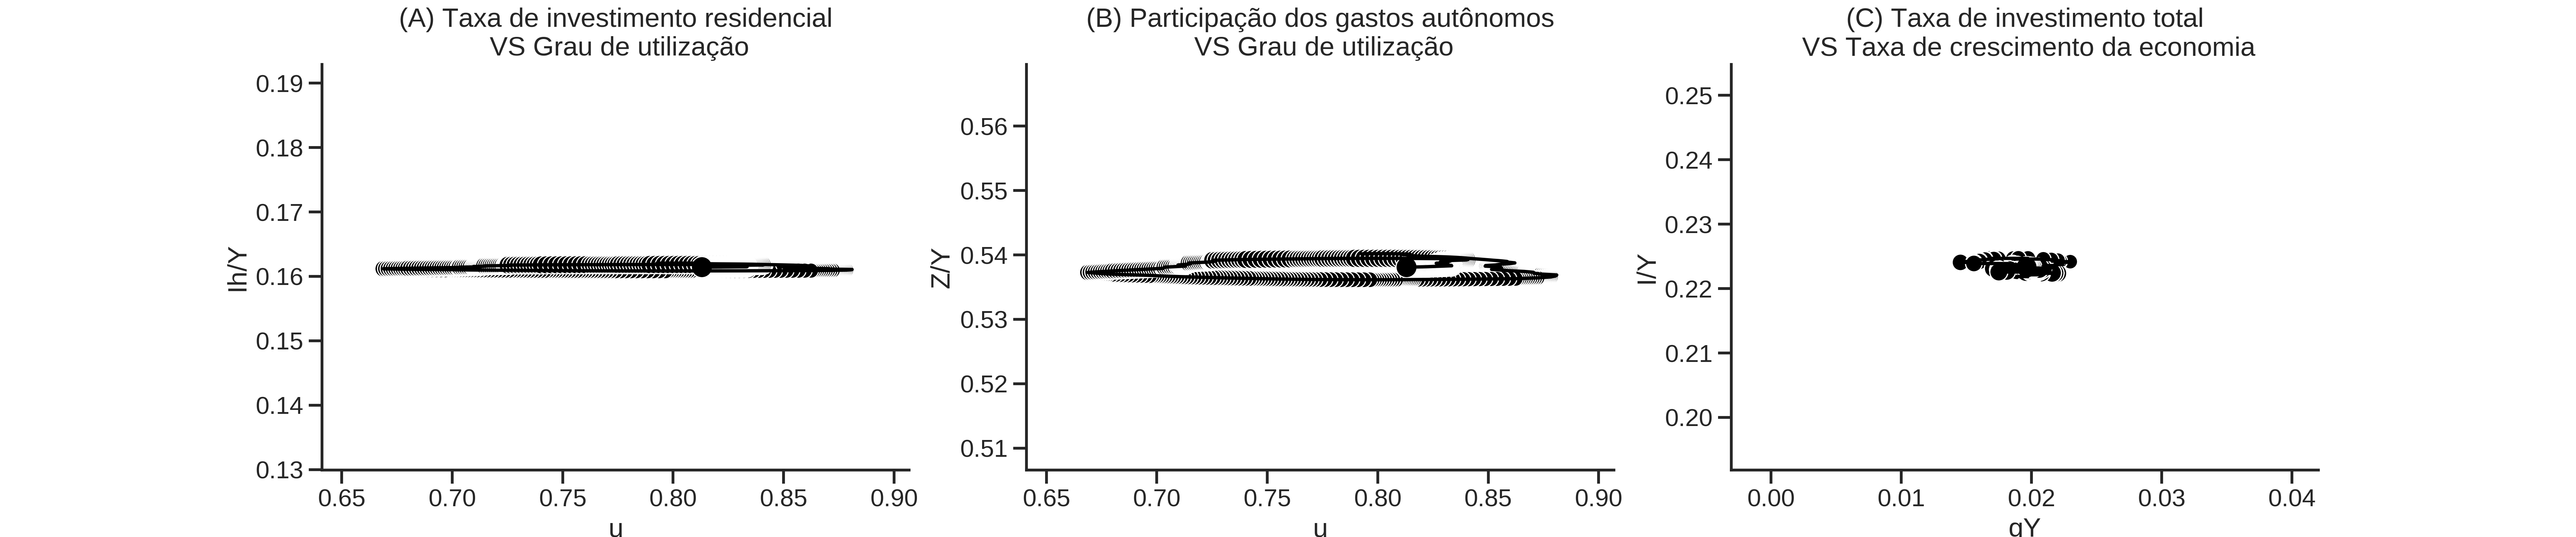
\includegraphics[width=\textwidth]{../../Modelo/Versoes/Clock_Real.png}
	\caption*{\textbf{Fonte:} Elaboração própria}
\end{figure}

Uma primeira aproximação é por meio do gráfico \ref{clock_Real} em que são apresentados --- como no gráfico \ref{FigIh_u} --- e  os gastos autônomos (somente investimento residencial e total) contra grau de utilização, bem como taxa de investimento total (firmas e famílias) e taxa de crescimento da economia.
Uma breve inspeção deste gráfico explicita a relação cíclica e horária entre participação dos gastos autônomos (tanto investimento residencial isolado quanto somado ao crédito aos capitalistas) e nível de atividade tal como discutido no capítulo anterior e o mesmo pode ser dito a respeito da taxa de investimento residencial e grau de utilização. Já o fato estilizado (1) não apresenta um padrão tão demarcado\footnote{A dificuldade de explicitar um padrão bem demarcado também decorre da volatilidade elevada de um dos eixos (taxa de crescimento) enquanto o outro é menos volátil (taxa de investimento).} uma vez que apresenta uma relação positiva entre taxa de investimento e de crescimento em alguns subperíodos e negativa em outros.

\begin{figure}[H]
	\centering
	\caption{Inserindo taxa de juros hipotecária e inflação de móveis observadas}
	\label{choque_Real}
	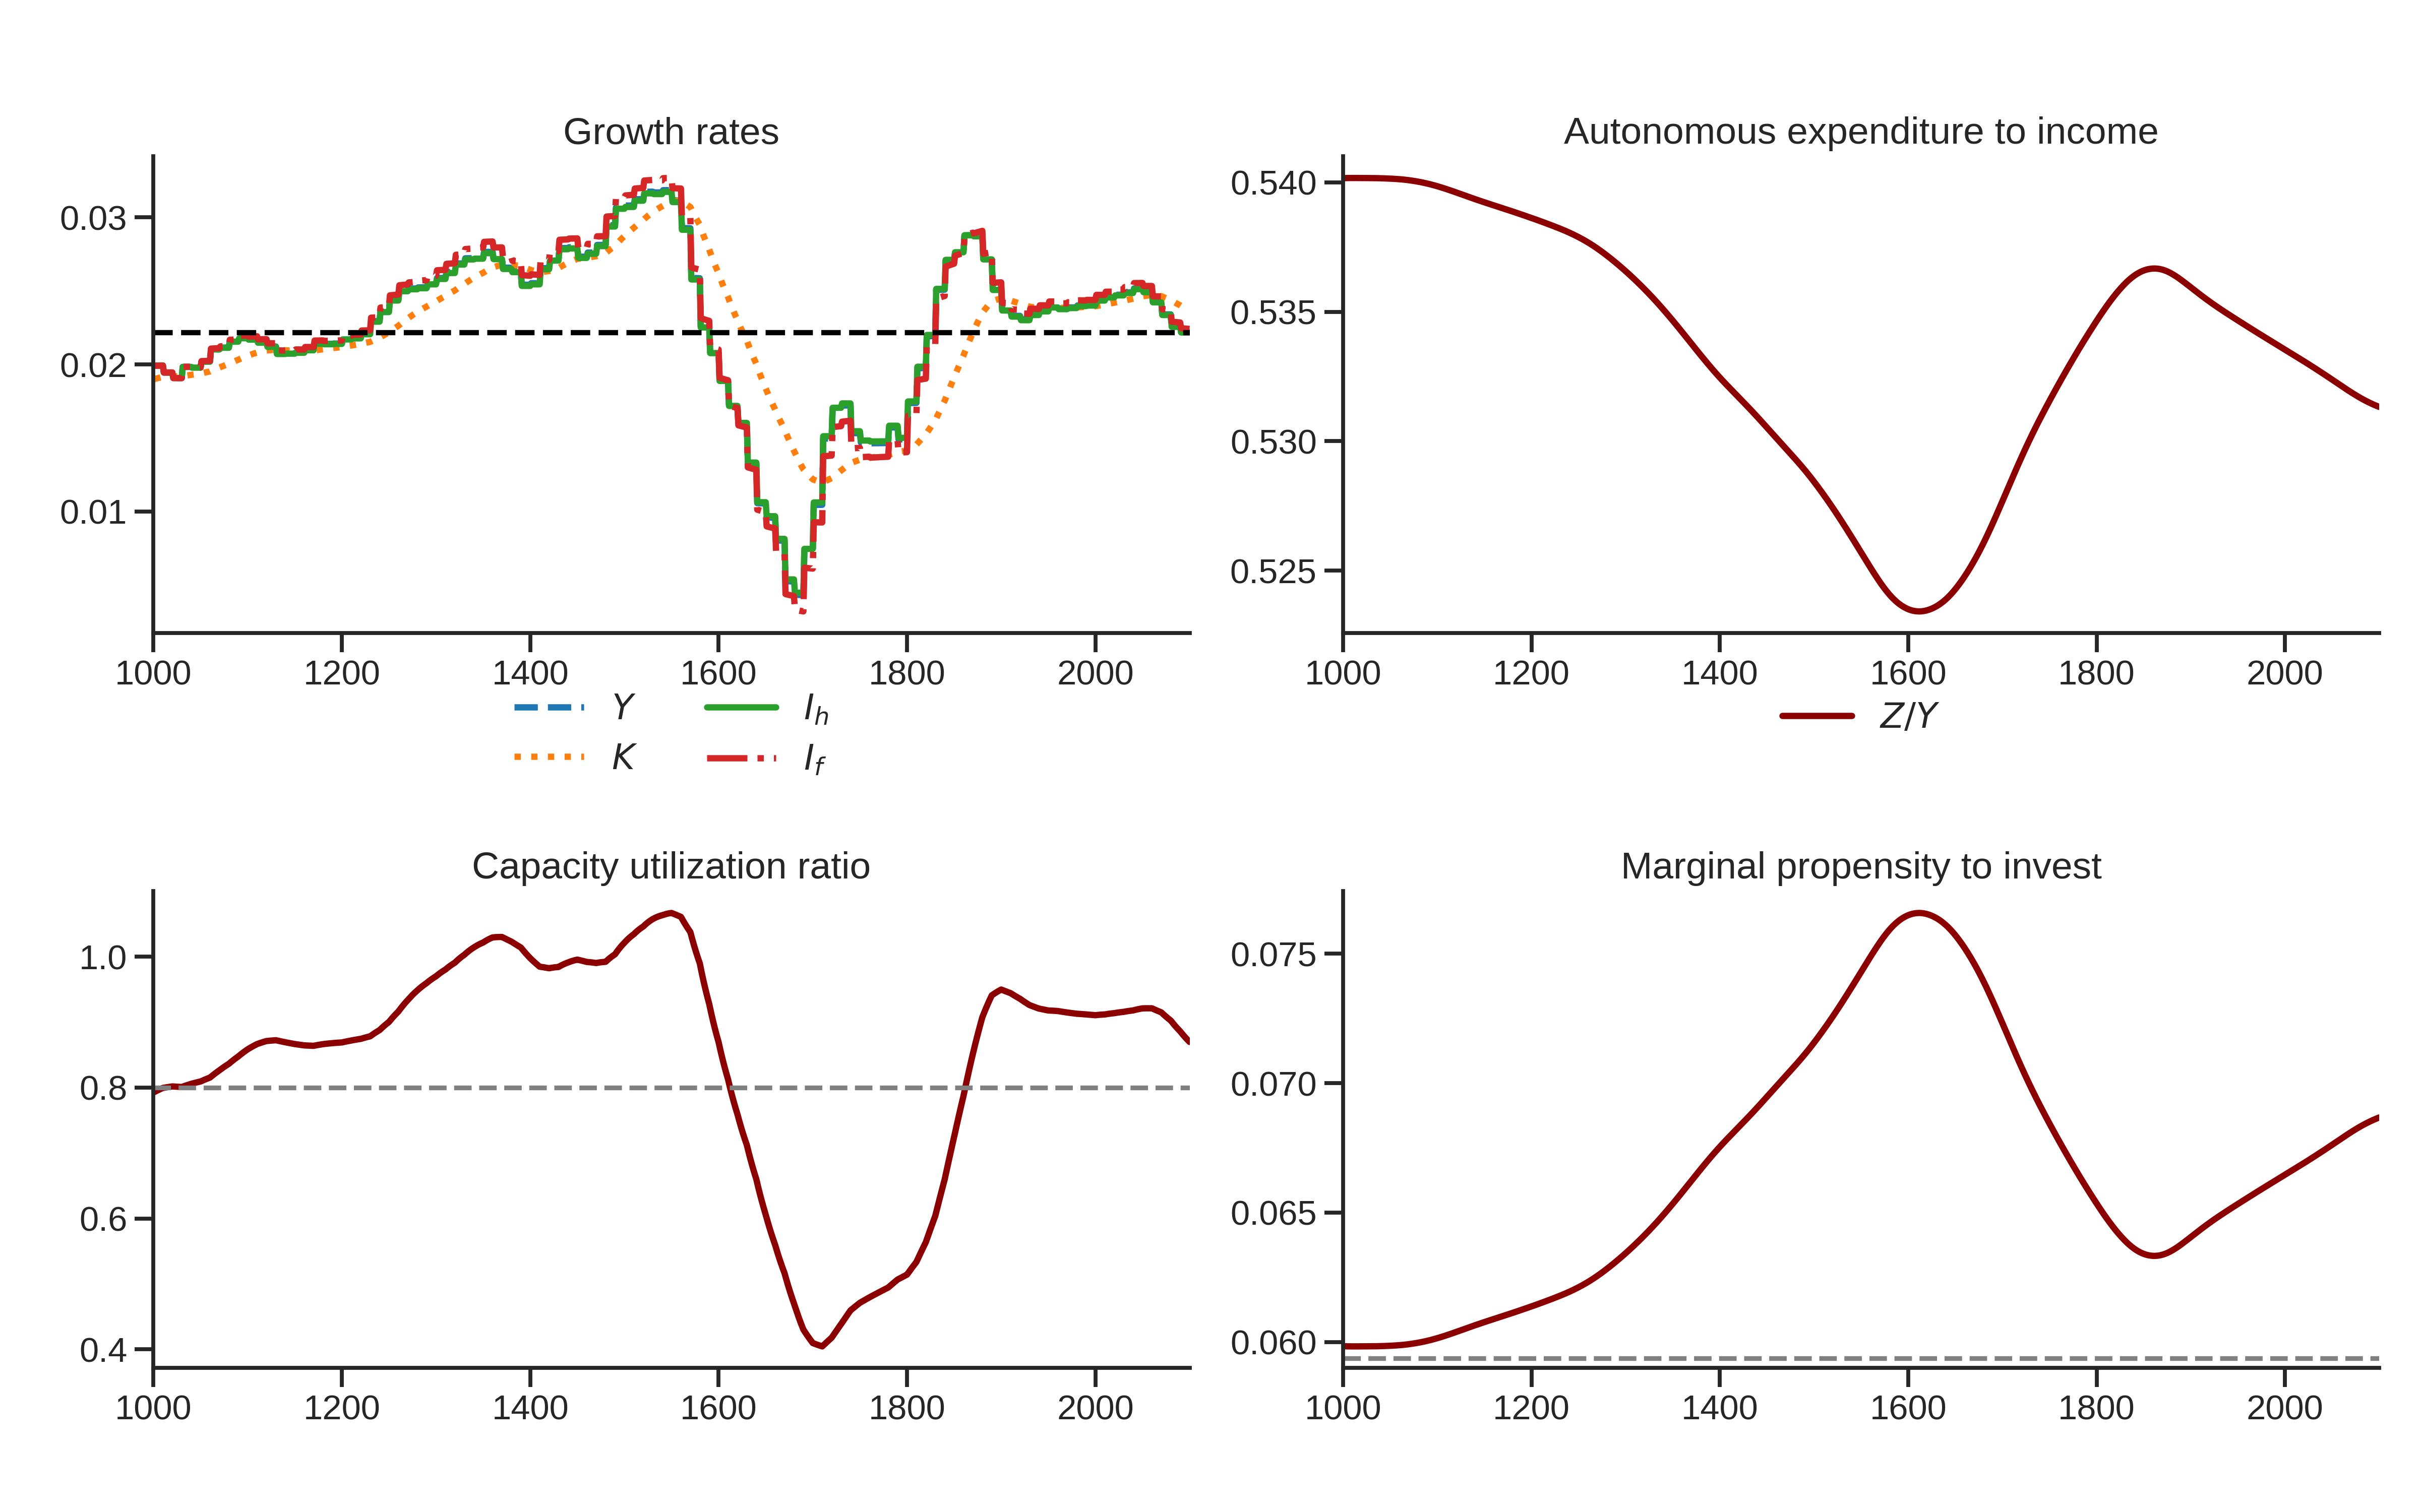
\includegraphics[width=\textwidth]{../../Modelo/Versoes/Shock_Real.png}
	\caption*{\textbf{Fonte:} Elaboração própria}
\end{figure}


O fato estilizado (2) referente ao grau de utilização é contemplado --- feitas as devidas mediações --- uma vez que o período analisado não corresponde a posição plenamente ajustada e, portanto, desvios no grau de utilização em relação ao normal são ajustados por meio de mudanças na propensão marginal a investir (fato estilizado 6). Por fim, destaca-se o acompanhamento da taxa de crescimento da economia aos gastos autônomos, notadamente investimento residencial. No entanto, não é capaz de replicar o fato estilizado (5) de maior volatilidade do investimento residencial.

\begin{figure}[H]
	\centering
	\caption{Inserindo taxa de juros hipotecária e inflação de móveis observadas}
	\label{choque_RealNorms}
	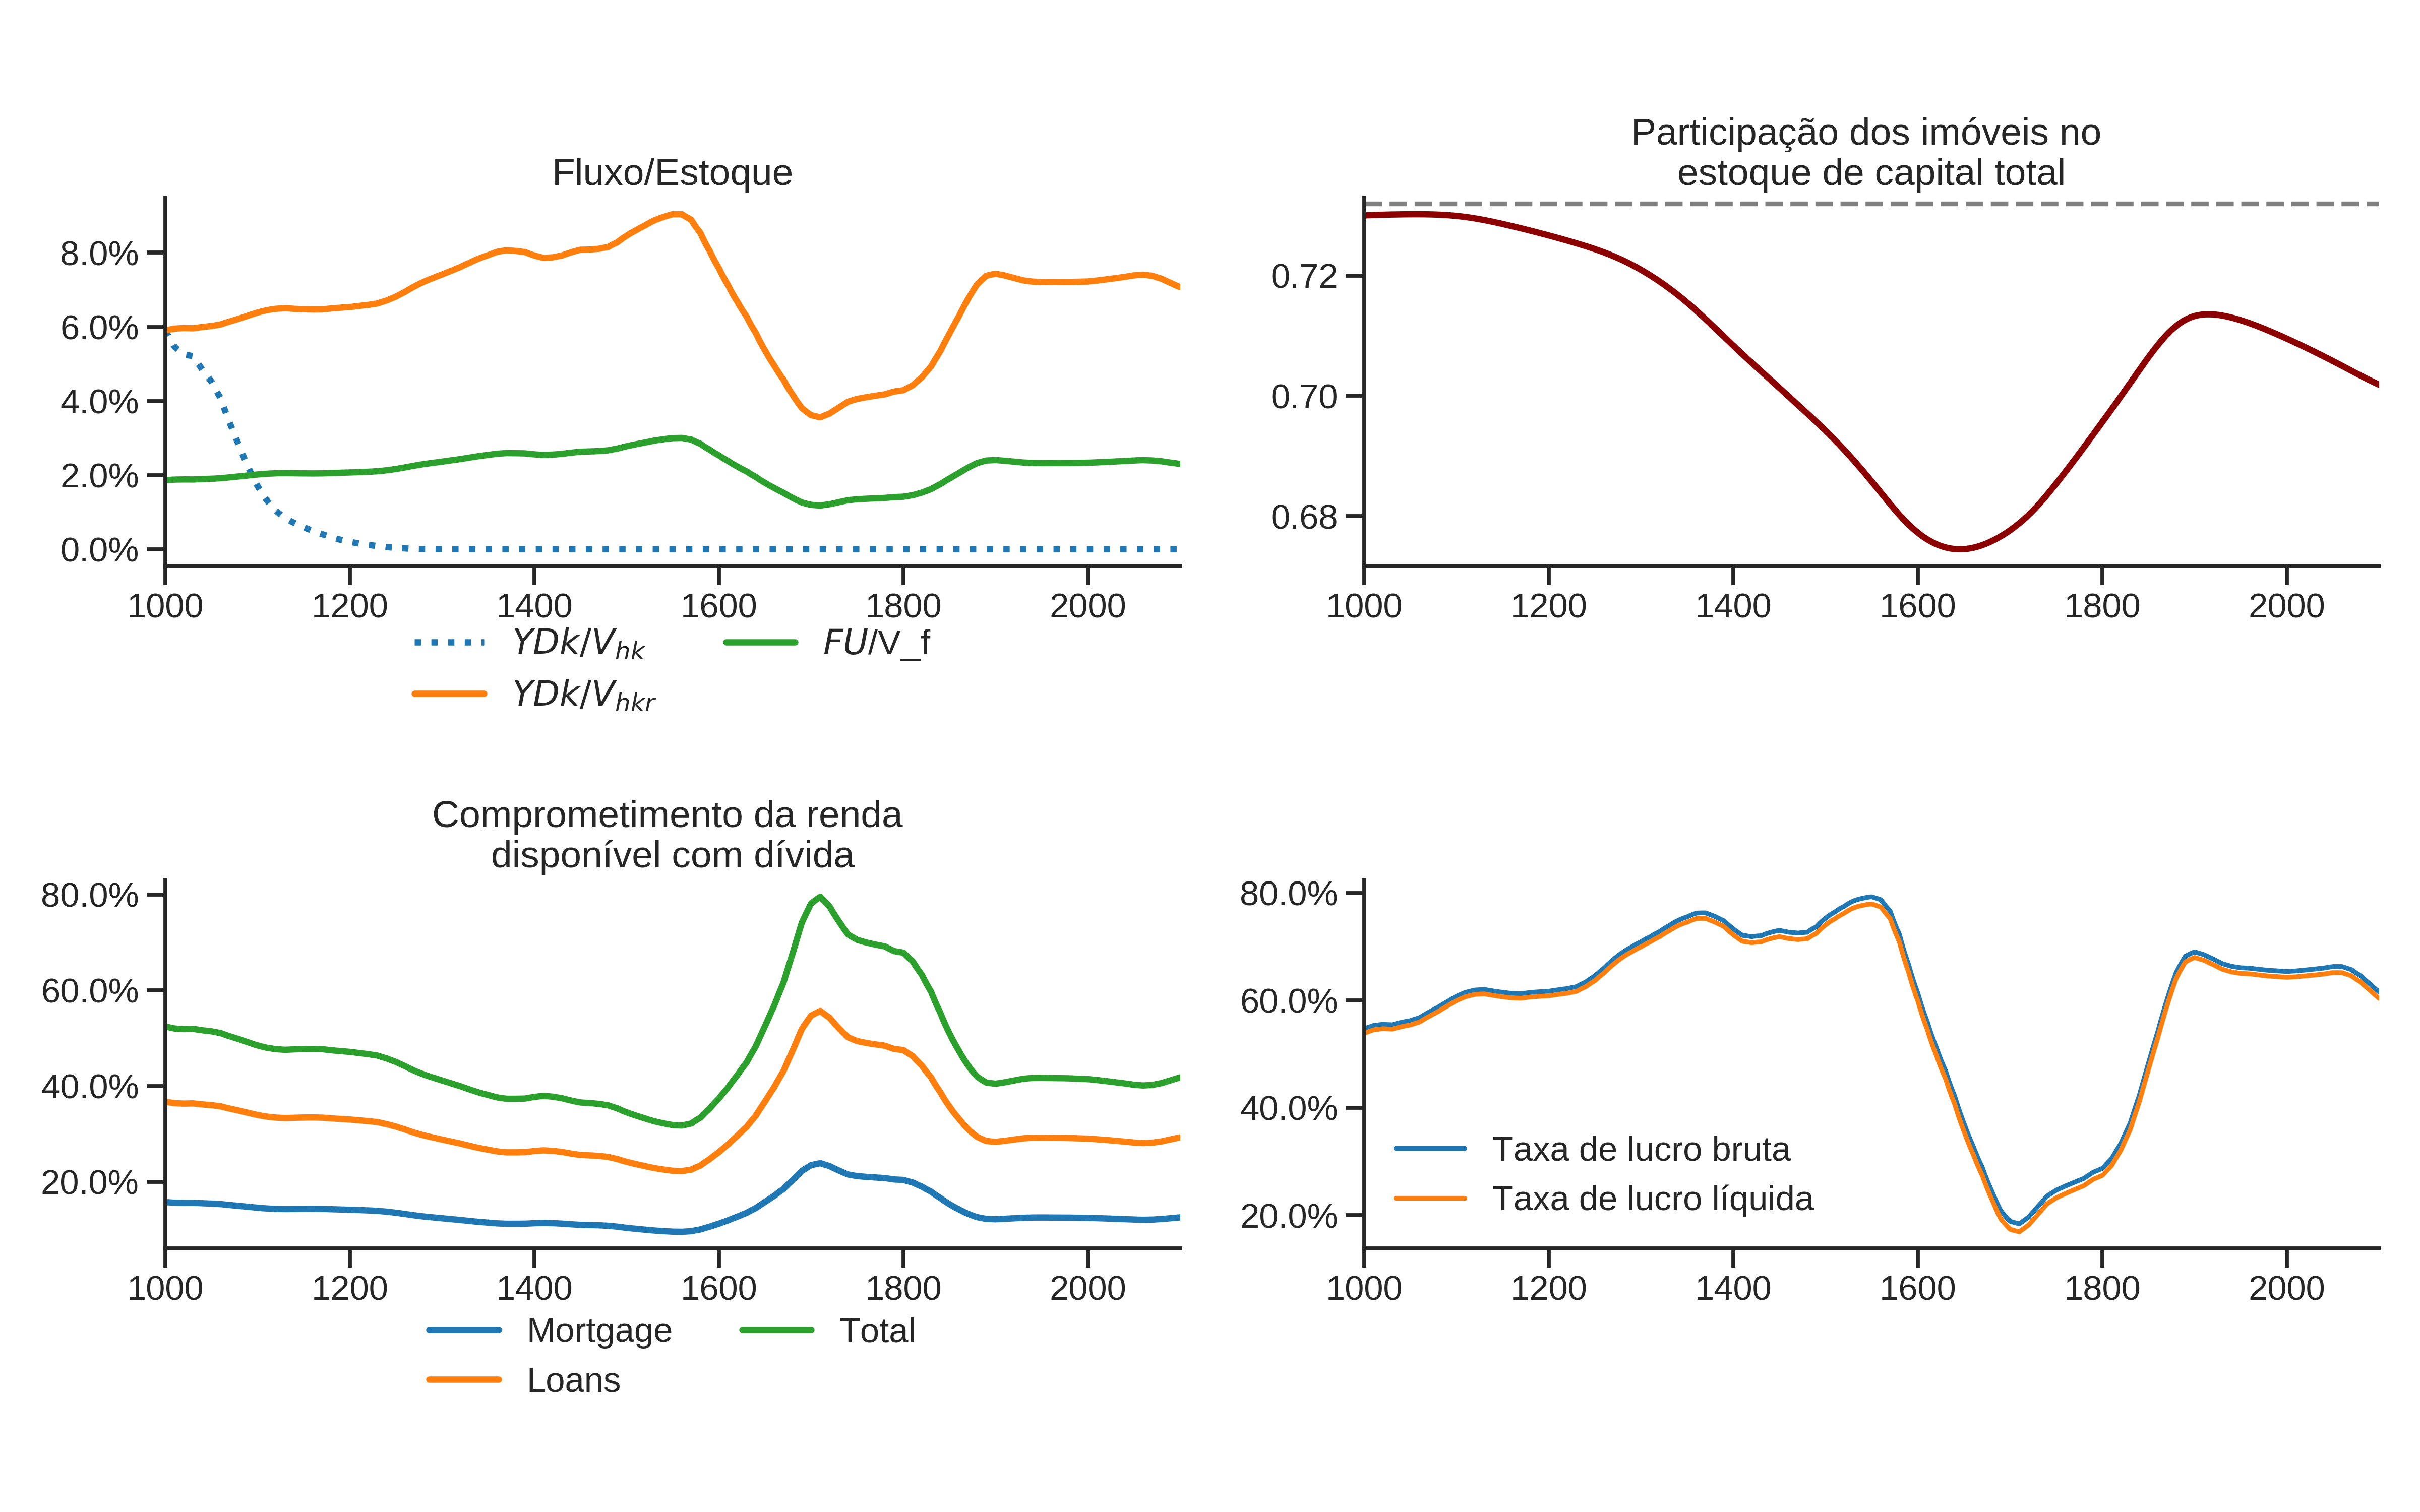
\includegraphics[width=\textwidth]{../../Modelo/Versoes/Shock_RealNorms.png}
	\caption*{\textbf{Fonte:} Elaboração própria}
\end{figure}

Por fim, destaca-se a reprodução do fato estilizado (3) em que tanto o comprometimento da renda das famílias com o pagamento de juros aumenta quanto a razão entre renda disponível em relação a riqueza diminui. Tal dinâmica de endividamento não teve um paralelo nas firmas uma vez que a taxa de lucro bruta e líquida se aproximaram no período equivalente a crise. 
%Além disso, esta simulação reproduz a redução nas taxas de lucro ao longo da crise que está associada a redução do nível de atividade --- dada a participação dos lucros na renda constante.
Vale lembrar que este é um primeiro esforço de confrontar um modelo teórico simulado com investimento residencial frente aos dados observados.
Além disso, tal procedimento não conta com a calibragem dos parâmetros e esta é uma frente de melhoria que versões futuras desta pesquisa pode seguir.
No entanto, os problemas decorrentes desta primeira tentativa de mediação entre teoria e empiria não se restrigem à calibragem. 
Apesar de lançar luz sobre alguns pontos destacados pela teoria, deixa outros em aberto e que devem ser aprimorados preservando as hipóteses do modelo:
\begin{description}
	\item[Temporalidade] Normalmente não é feita uma distinção/discussão nos modelos do tipo SFC de simulação sobre o significado econômico das defasagens adotadas. Sendo assim, para que um modelo teórico tenha maior aderência a empiria é preciso repensar o significado da temporalidade de algumas variáveis;
	\item[Grau de utilização normal] Ao longo desta pesquisa, adotou-se um grau de utilização normal arbitrário (e constante) que, por sua vez, não equivale --- necessariamente --- à média ou à tendência do grau de utilização efetivo. Desse modo, é preciso avançar em direção às formas de incluir tal conceito nos modelos sem que, para isso, seja necessário endogeneizá-lo;
	%incorrer em imprecisões teóricas nem se restringir a arbitrariedade;
	\item[Participação dos gastos autônomos] Tal como o grau de utilização normal, a escolha da participação dos gastos autônomos ($R$) também é arbitrária. Se faz necessário investigar formas de endogeneizar tal participação sem incorrer em soluções assintóticas em que a parcela de um dos gastos convirja a zero;
	\item[Saldo líquido dos setores] Por se tratar de uma economia fechada sem governo, se as famílias forem deficitárias neste modelo as firmas serão necessariamente superavitárias (e o inverso também é válido).
	Sendo assim, para que esta dualidade não seja a única combinação possível se faz necessário incluir outros setores institucionais. No entanto, versões futuras desta pesquisa irão avançar neste nível de complexidade se acrescentar elementos relevantes tanto para a dinâmica do investimento residencial quanto para as implicações macroeconômicas deste gasto. Caso contrário, tais modificações adicionarão complexidade sem incluir --- necessariamente --- maior esclarecimento;
	\item[Composição do patrimônio líquido dos bancos] Ao longo deste capítulo adotou-se a hipótese que os bancos não auferem lucros e, por consequência, não acumulam ativos.
	Sendo assim, tal modelo não consegue reproduzir --- por construção --- razões entre ativos/passivos sobre o patrimônio líquido uma vez que a riqueza (total e financeira) deste setor institucional é nula.
	Desse modo, para que seja capaz de replicar mudanças na composição do patrimônio líquido dos bancos é preciso que este setor passe a obter lucros que, por sua vez, rompe com as hipóteses aqui adotadas.
\end{description}

\section{Considerações finais}\label{Conclusao_Modelo}

Por mais que algumas questões precisam ser melhor desenvolvidas, pontua-se que 
esta pesquisa contribuiu para a literatura de crescimento liderado pela demanda do modelo do supermultiplicador sraffiano, levando em consideração o esforço recente de incorporá-lo em um arcabouço contábil do tipo SFC.  A característica específica do modelo aqui apresentado é a inclusão do investimento residencial. A introdução desse gasto teve como objetivo dar conta dos resultados de alguns trabalhos empíricos recentes que mostram a importância do investimento residencial para dinâmica macroeconômica e, como visto anteriormente, nenhum trabalho havia simulado esse gasto específico via taxa própria de juros dos imóveis. 

O modelo reproduz as principais características do supermultiplicador sraffiano: (i) o grau de utilização converge ao grau normal, por meio de variações da propensão marginal a investir das firmas e; (ii) a taxa de crescimento da economia segue a taxa de crescimento dos gastos autônomos --- nesse caso, o investimento residencial. A primeira diferença do  presente modelo é que o estoque de capital fixo da economia passa a ter dois componentes, o capital produtivo das firmas e os imóveis das famílias. 

Como visto nas simulações, o principal resultado particular deste modelo é que uma maior taxa de crescimento do investimento residencial tem como consequência uma redução da participação do estoque de imóveis no capital total. Tal resultado, aparentemente contra intuitivo, se deve ao ajuste do estoque de capital das firmas. Para que o grau efetivo de utilização da capacidade convirja ao grau normal, o investimento das firmas precisa temporariamente crescer mais rápido que investimento residencial, alterando, portanto, a relação entre os dois estoques. 

Os outros dois experimentos trazem resultados em linha com o supermultiplicador sraffiano. A diminuição da participação dos salários na renda não afeta a taxa de crescimento de longo prazo e, portanto, não afeta a propensão marginal a investir de forma permanente. Porém, por alterar o tamanho do supermultiplicador, diminui a participação do capital produtivo no capital total. O aumento da taxa de juros, por sua vez, tem um efeito tanto sobre a taxa de crescimento de longo prazo quanto sobre o endividamento das famílias em relação à renda disponível. 

É importante destacar que este trabalho é apenas o primeiro passo numa agenda de pesquisa mais ampla sobre o papel do investimento residencial no ciclo e no crescimento econômico. Pesquisas futuras podem (e devem) tornar o modelo aqui apresentado mais complexo. Possíveis extensões incluem explorar outros determinantes do investimento residencial bem como seus impactos sobre outros gastos autônomos e sobre o patrimônio líquido dos bancos.
Com isso, concluí-se os objetivos pretendidos com o modelo apresentado. Cabe ao capítulo seguinte reunir as conclusões desta pesquisa e alguns direcionamentos futuros.


%=====================================================================
% 							Bibliografia
%=====================================================================
%{\let\clearpage\relax \chapter{Bibliografia}}
%-----

\SingleSpacing

{\let\clearpage\relax\printbibliography}

%\begin{table}
\caption{Selection model order (* indicates the minimum)}
\label{criterios}
\centering
\begin{tabular}{lcccc}
\toprule
            & \textbf{AIC} & \textbf{BIC} & \textbf{FPE} & \textbf{HQIC}  \\
\midrule
\textbf{0}  &      -13.86  &      -13.71  &   9.553e-07  &       -13.80   \\
\textbf{1}  &      -14.71  &     -14.46*  &   4.102e-07  &       -14.61   \\
\textbf{2}  &      -14.72  &      -14.38  &   4.038e-07  &       -14.58   \\
\textbf{3}  &      -14.74  &      -14.29  &   3.983e-07  &       -14.56   \\
\textbf{4}  &      -14.88  &      -14.34  &   3.442e-07  &      -14.66*   \\
\textbf{5}  &     -14.89*  &      -14.24  &  3.425e-07*  &       -14.63   \\
\textbf{6}  &      -14.84  &      -14.09  &   3.612e-07  &       -14.54   \\
\textbf{7}  &      -14.82  &      -13.97  &   3.696e-07  &       -14.47   \\
\textbf{8}  &      -14.77  &      -13.82  &   3.891e-07  &       -14.38   \\
\textbf{9}  &      -14.75  &      -13.71  &   3.961e-07  &       -14.33   \\
\textbf{10} &      -14.70  &      -13.56  &   4.189e-07  &       -14.24   \\
\textbf{11} &      -14.67  &      -13.43  &   4.308e-07  &       -14.17   \\
\textbf{12} &      -14.63  &      -13.29  &   4.535e-07  &       -14.08   \\
\textbf{13} &      -14.66  &      -13.22  &   4.406e-07  &       -14.08   \\
\textbf{14} &      -14.63  &      -13.09  &   4.582e-07  &       -14.00   \\
\textbf{15} &      -14.59  &      -12.95  &   4.806e-07  &       -13.92   \\
\bottomrule
\end{tabular}
\caption*{\textbf{Source:} Authors' elaboration}
\end{table}


%\input{AnexoB.tex}



\end{document}